\documentclass[11pt,a4paper,twoside]{book}
% Specifies the directory where pictures are stored
\usepackage[utf8]{inputenc}
\usepackage[T1]{fontenc}
\usepackage[french]{babel}
\usepackage{amsmath}
\usepackage{amsfonts}
\usepackage{amssymb}
\usepackage{color}
\usepackage{graphicx}
\usepackage{float}
\usepackage{hyperref}
\usepackage{listings}
\usepackage{makeidx}
\usepackage{fancyhdr}
\usepackage{setspace}
\usepackage{longtable}
\usepackage{vmargin}

\hypersetup{urlcolor=black, colorlinks=true}
%*************************************************
%----------------------------------------------------------------------------------------
% MARGINS
%----------------------------------------------------------------------------------------
\setmarginsrb  { 1.5in}  % left margin
                        { 0.6in}  % top margin
                        { 1.0in}  % right margin
                        { 0.8in}  % bottom margin
                        {  20pt}  % head height
                        {0.25in}  % head sep
                        {   9pt}  % foot height
                        { 0.3in}  % foot sep
%----------------------------------------------------------------------------------------
% COMMANDS
\lhead[\rm\thepage]{\fancyplain{}{\sl{\rightmark}}}
\newcommand\bhrule{\typeout{------------------------------------------------------------------------------}}
\newcommand\btypeout[1]{\bhrule\typeout{\space #1}\bhrule}
\newcommand\listofsymbols[2]{
\btypeout{\listsymbolname}
\addtotoc{\listsymbolname}
    \chapter*{\listsymbolname
      \@mkboth{
          \MakeUppercase\listsymbolname}{\MakeUppercase\listsymbolname}}
\begin{longtable}[c]{#1}#2\end{longtable}\par
    \cleardoublepage
}
% *****************
\setlength{\parindent}{0pt} 
\setlength{\parskip}{2.0ex plus0.5ex minus0.5ex}%plus0.5ex minus0.2ex} 

\lstset{captionpos=b,
        breaklines=true
        frame=tb,
        basicstyle=\scriptsize\ttfamily,
        showstringspaces=false,
        keepspaces=true}
\lstdefinestyle{matlab} {
        language=Matlab,
        keywordstyle=\color{blue},
        commentstyle=\color[rgb]{0.13,0.55,0.13}\em,
        stringstyle=\color[rgb]{0.7,0,0} }
%********************************************************
\begin{document}
\renewcommand{\labelitemi}{$\bullet$}
\frontmatter
\fancyhead{}
\pagestyle{fancy}
\graphicspath{{Pictures/}}
\setstretch{1.3} 

\author{Xavier Crochet}
\title{Automatisation de la gestion des programmes de cours}
\date{June 2013}
\frontmatter
\begin{titlepage}
\begin{center}
\begin{minipage}{0.4\textwidth}
\begin{flushleft} \large

\includegraphics[width=0.6\textwidth]{ucl}
\end{flushleft}
\end{minipage}
\begin{minipage}{0.4\textwidth}
\begin{flushright}

\includegraphics[width=0.6\textwidth]{epl}
\end{flushright}
\end{minipage}
\vfill
Université Catholique de Louvain \\
Louvain School of Engineering \\
Department of Computer Engineering
\vfill
%\\%[1.2cm]
\textsc{\LARGE Automatisation de la gestion des programmes de cours}%\\%[1.2cm]
\vfill
\emph{Auteur}\\
\large{Xavier \textsc{Crochet}}
\vfill
\begin{minipage}{0.4\textwidth}
\begin{flushleft} \large
\emph{Promoteurs}\\Kim \textsc{Mens}\\
Chantal \textsc{Poncin}\\
\emph{Lecteur}\\Bernard \textsc{Lambeau}\\
\end{flushleft}
\end{minipage}
\begin{minipage}{0.4\textwidth}
\begin{flushright} \large
Mémoire présenté dans le cadre du \emph{Master 120} en \emph{Sciences Informatiques} option \emph{sécurité et réseaux}
\end{flushright}
\end{minipage}
\vfill
Louvain-la-Neuve\\
{\large Juin 2014}
\end{center}
\end{titlepage}
\newpage
\vspace*{\fill}
\begin{center}
\begin{minipage}{0.4\textwidth}
\begin{flushright} \large
Un grand merci à Chantal Poncin et à Kim mens pour leur support, conseils et excellente disponibilité.
\end{flushright}
\end{minipage}
\end{center}
\vspace*{\fill}

%\frontmatter
\tableofcontents
%\include{preface}

\clearpage
\setstretch{1.5} 
\lhead {\emph{Abréviations}}

\begin{longtable}{c c}

\textbf{FWB} & \textbf{F}édération \textbf{W}allonie - \textbf{B}ruxelles\\
\textbf{Commission INFO} & Commission de Programme du département\\ 
&d'informatique de l'école polytechnique de Louvain -là-Neuve\\
\textbf{Module} & Ensemble de cours, obligatoire ou non\\
& Ex: L'option intelligence artificielle dans le programme de master\\
\textbf{EPC} & \textbf{E}tudiant \textbf{P}rogramme \textbf{C}ours\\
&Outil de gestion du parcours étudiant de l’UCL\\
\textbf{Rails} & Ruby On Rails\\
%\textbf{Acronym} & \textbf{W}hat (it) \textbf{S}tands \textbf{F}or \\
\end{longtable}

 


\mainmatter
% add intro
\chapter{Introduction}
\label{introduction}
\lhead{Chapitre 1 - Introduction}
\section{Contexte}

Chaque année à l'Université catholique de Louvain, et dans toutes les autres universités, un étudiant est amené à devoir effectuer des choix au niveau du programme de cours qu'il va suivre. Même si ces choix demeurent plus restreints en bac qu'en master, le processus actuel représente une lourde tâche de travail pour le personnel en charge de la vérification de ces programmes et risque de s'amplifier encore plus avec le nouveau décret. 

En bachelier, cela se limite au choix d'une mineure de manière générale. La tâche est déjà plus compliquée lorsqu'il faut traiter le programme d'un étudiant qui recommence son année.

En master par contre, l'ensemble des choix est plus vaste. Le catalogue des programmes est plus versatile (Master 120, Master 60) et plus modulable. En effet, un étudiant doit choisir une ou plusieurs options. De plus, chacune d'entre elles est composée de cours obligatoires et optionnels. Ensuite, pour les programmes étalés sur deux ans, chacun des cours peut être suivi durant la première ou la deuxième année. Enfin, il faut prendre en compte les diverses équivalences lorsqu'un étudiant de notre faculté part en Erasmus, ou lorsqu'un étudiant étranger vient étudier dans notre université. Le processus de validation est donc plus complexe et nécessite considérablement plus de temps pour chacune des deux parties, à savoir la commission de programme du département d'informatique de l'École Polytechnique de Louvain - (\textbf{La commission INFO}) - et ses étudiants. 

En outre, la fédération Wallonie - Bruxelles (\textit{FWB}) a réalisé un décret qui a un impacte considérable sur comment, quand les étudiants  peuvent et doivent créer leur programme et choisir leur cours. Le but de cette réforme est de proposer des programmes plus à la carte,  afin que la structure des formations enseignées chez nous se calque sur celle des grandes universités anglo-saxonnes.

Cette réforme a pour conséquence de complexifier la gestion des programmes de master, mais surtout ceux de bachelier, offrant plus de liberté aux étudiants. Alors que le gros du travail se fait actuellement à l'aide d'un formulaire papier, il est urgent de passer à une version automatique pour simplifier la tâche au personnel et aux étudiants. 

\clearpage
\section{Problème}
Le problème est, une fois découpé, relativement simple à comprendre. Nous avons deux acteurs; \textit{la commission INFO} et les étudiants. 
La \textit{commission INFO} propose un catalogue de cours aux étudiants et plusieurs types de contraintes s'exercent sur chacun des cours de ce catalogue. L'étudiant doit se construire un programme de cours à partir du catalogue et \textit{la commission INFO} doit vérifier l'intégrité du programme de chaque étudiant. Il y a donc un processus de \textit{négociation} entre les deux parties, durant lequel \textit{la commission INFO} souligne les erreurs éventuelles pour être, par après,  corrigées par l'étudiant jusqu'à la validation de son programme.

Cependant, il faut garder à l'esprit que l'état du catalogue, des contraintes ou même des cours peut évoluer à tout moment. Comme mentionné plus haut, la \textit{FWB} peut émettre de nouvelles règles, de nouvelles lois dont l'impact peut bouleverser de façon relativement importante la structure et l'organisation des programmes. De plus, il est fréquent de voir certaines contraintes, comme les crédits d'un cours, le semestre ou même le cycle durant lequel il est dispensé, changer au cours des années.

L'encodage, l'interprétation, la connaissance et la vérification de l'ensemble de ces contraintes, qui ne sont parfois pas très explicites, sont à la charge de \textit{la commission INFO}.

L'image~\ref{fig:master_program} représente une vue de l'ensemble des cours, modules et contraintes du programme de \textbf{master} en informatique. Les nœuds représentent les différents cours, modules et programmes disponibles, tandis que les liens entre ces différents nœuds correspondent aux dépendances entres les cours. La complexité du graphe, malgré qu'il a été retravaillé et simplifié pour augmenter sa lisibilité, est assez évidente.

\begin{figure}
\centering
\caption{Programme de Master}
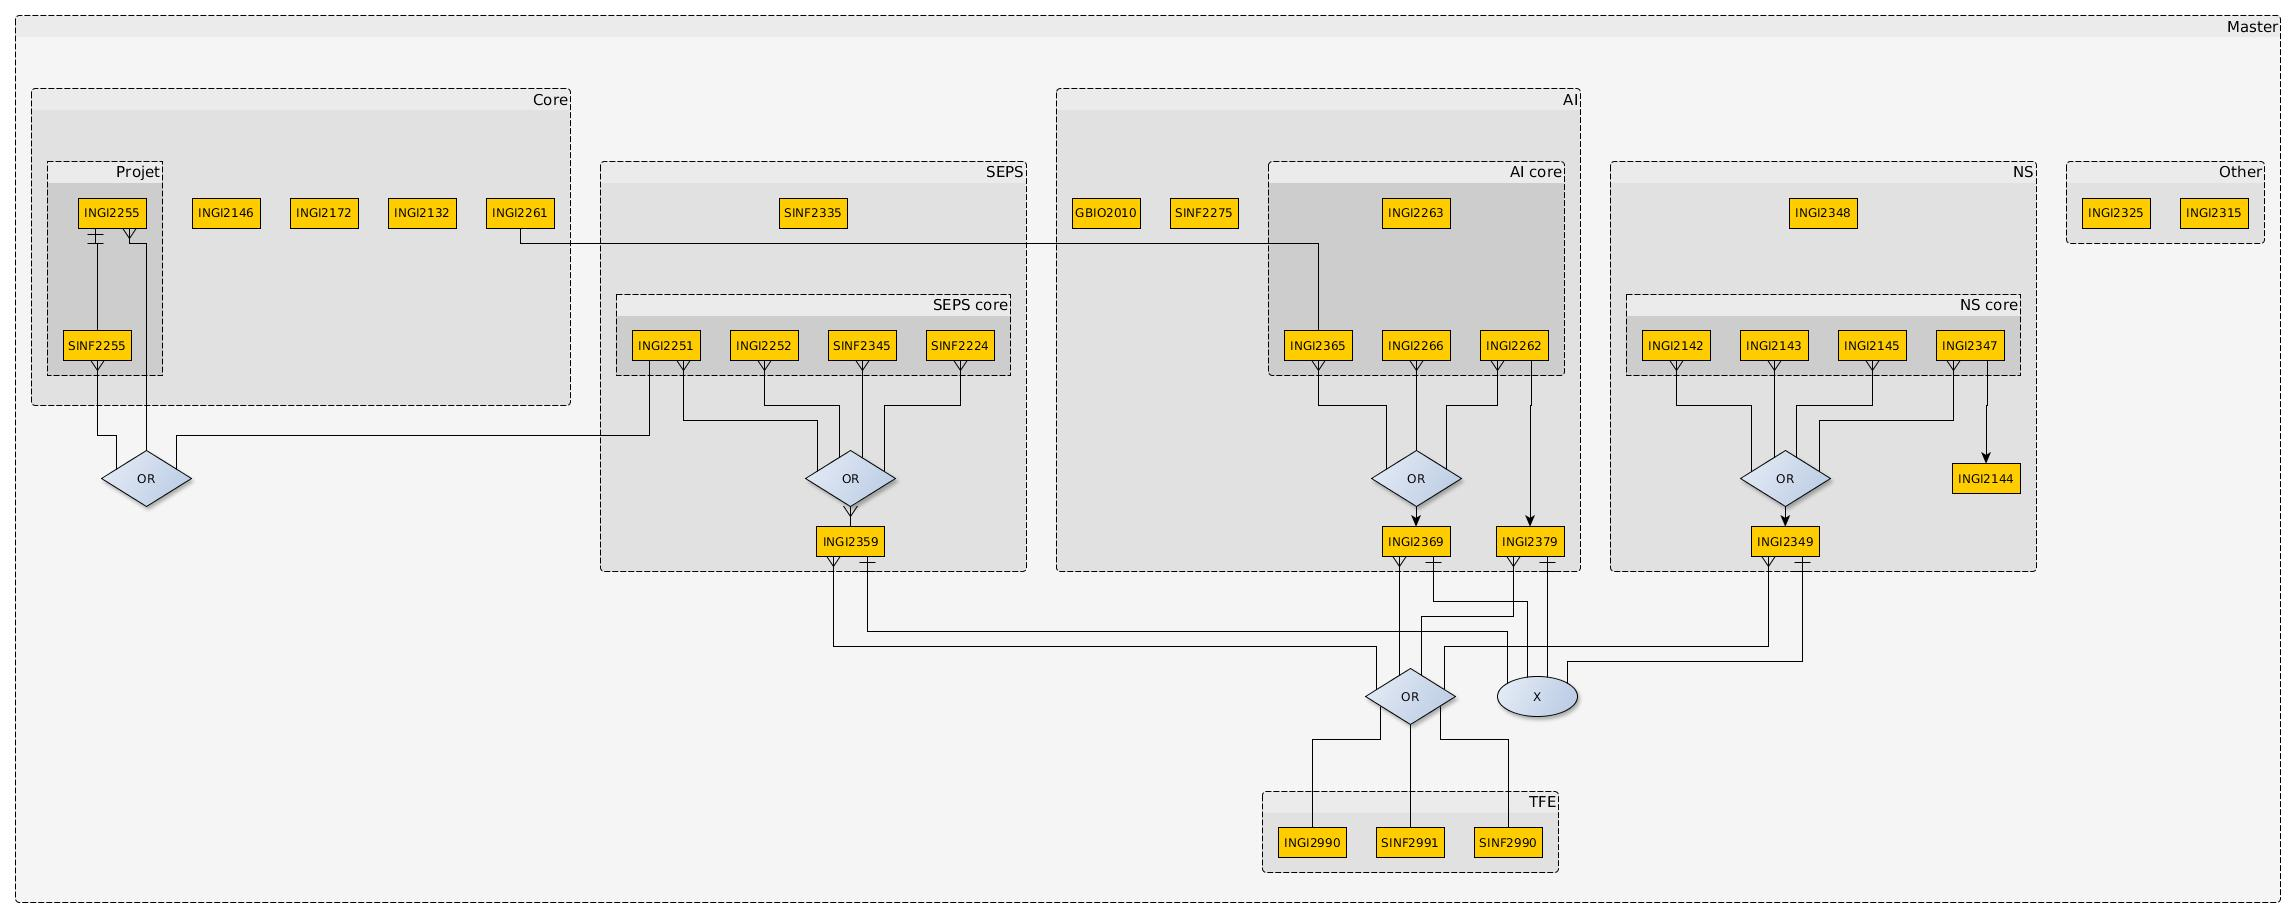
\includegraphics[angle=90, height=0.95\textheight, width=0.9\textwidth]{master_program}
\label{fig:master_program}
\end{figure}

Présentement, le processus de construction du programme de cours pour un étudiant est assez rudimentaire. Ce processus est représenté sur le diagramme ~\ref{fig:initial_process}

\begin{figure}
\centering
\caption{Processus actuel}
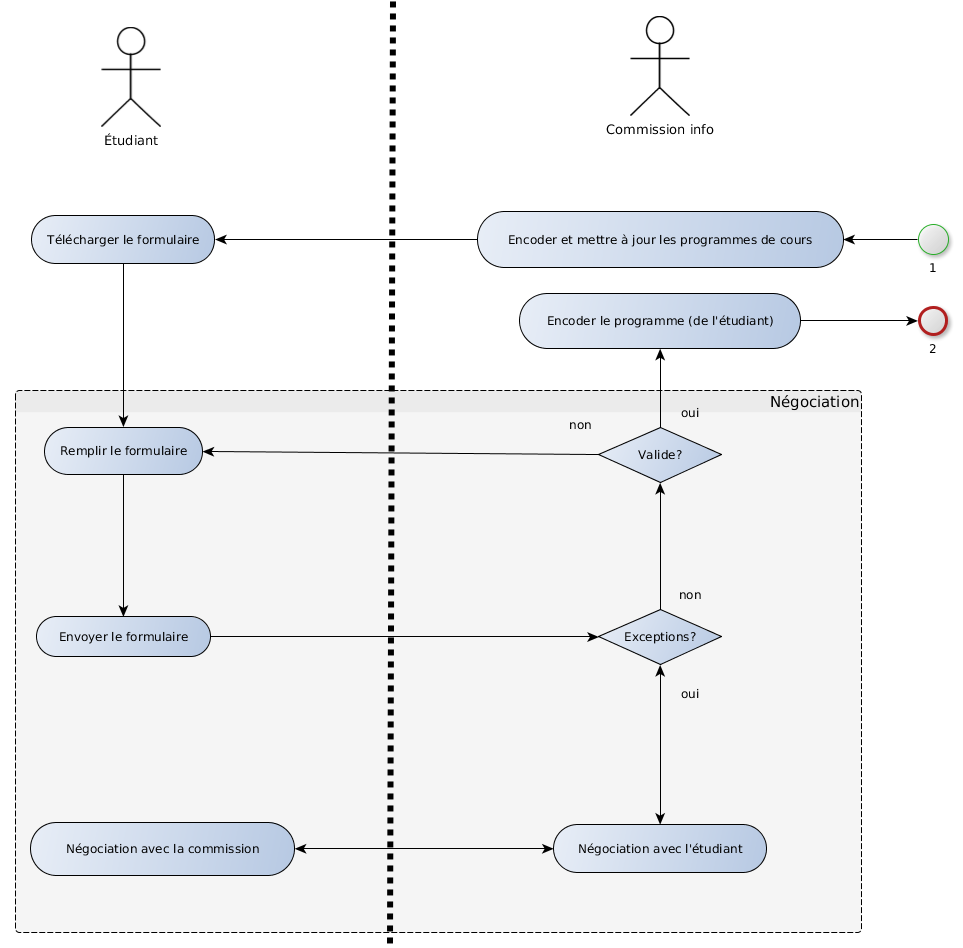
\includegraphics[width=\textwidth]{initial_process}
\label{fig:initial_process}
\end{figure} 

\textit{La commission INFO} commence par mettre à jour ses différents programmes de cours, puis crée le formulaire excel contenant le programme de cours et enfin le mets en ligne sur le portail de la faculté (afin qu'il soit téléchargeable par les étudiants par après).

L'étudiant télécharge le formulaire contenant le programme de cours et le remplit. 

Ici commence la phase de négociation entre \textit{la commission INFO} et les étudiants. Les deux parties vont s'échanger un formulaire que l'étudiant va compléter et \textit{la commission INFO} vérifier. L'échange va se poursuivre jusqu'à ce que le programme soit valide. 

L'étudiant complète d'abord son formulaire en tenant compte des spécifications du programme. S'il est en bac par exemple, il y a des cours obligatoire à prendre chaque année. S'il est en master, il y a une option à choisir, des cours obligatoires, etc. Il peut cependant exister des exceptions dans les différents programmes qui permettent d'enfreindre ces spécifications. Par exemple, un étudiant en provenance d'une autre université ou d'une autre faculté peut avoir déjà suivit l'équivalent d'un cours obligatoire dans son université ou sa faculté d'origine. Il va devoir rendre un formulaire qui ne respecte pas les contraintes initiales, justifier ces exceptions et négocier leur acceptation avec \textit{la commission INFO}.

Il envoie son formulaire par mail à \textit{la commission INFO}.

\textit{La commission INFO} réceptionne le formulaire. Elle vérifie la validité du programme. Si l'étudiant revendique des exceptions dans son programme, elle vérifie si elle sont fondées ou non. Si le programme ou ces exceptions ne sont pas validées, la \textit{commission INFO} peut demander d'amples informations à l'étudiant ou négocier avec lui et, si nécessaire, il est demandé à l'étudiant de compléter sont formulaire avec les informations qu'il manque. Le processus de validation recommence ainsi à zéro. Si le programme est valide, il est encodé. 

Le processus actuel, que ce soit en bac ou en master, se déroule essentiellement à l'aide d'une feuille de papier et les négociations par mail ou oralement. L'étudiant recherche les informations dont il a besoin sur le site de l'UCL, auprès de ses collègues ou encore sur les forums de cours, complète le formulaire et le dépose au secrétariat.

\textit{La commission INFO} quant à elle, effectue une vérification à la main de ces formulaires, négocie oralement ou par mail avec les étudiants si besoin est. 
Informatiser ce processus à l'air du web 3.0 est une nécessite plus qu'absolue.



\section{Motivation}
Reprenons le diagramme \ref{fig:initial_process} représentant le processus de création de programme tel qu'il se déroule actuellement. 

Le mot d'ordre est \textbf{automatisation}.

Comme présenté dans la section précédente, certaines étapes sont sources de beaucoup de problèmes pour \textit{la commission INFO}.

\begin{description}
  \item[Encodage/Mise à jour des programmes de cours] Cette étape se fait manuellement. De plus, la \textit{ commission INFO} doit, une fois le programme encodé, compléter à la main le formulaire excel qui va être utilisé par les étudiants. 
  \item[Vérification des programmes des étudiants]  Cette étape se fait manuellement. 
  \item[Négociation avec les étudiants] Cette étape se fait oralement ou par mails.
\end{description} 

Avant toute chose, il y a beaucoup d'informations qui sont échangées entre les deux parties, que ce soit implicitement ou explicitement.

Les données implicites correspondent aux informations relatives aux étudiants, comme l'historique de leur parcours universitaire, qui pourrait par exemple justifier certaines des exceptions mentionnées précédemment. Ces données ne concernent pas directement les choix faits par les étudiants au niveau de leur programme de cours, mais sont plutôt des méta-informations qui complètent leur profile. 

Les données explicites correspondent aux choix faits par les étudiants. Ces données concernent les
\begin{itemize}
\item les choix faits par les étudiants au niveau de leur programme de cours;
\item les justifications des étudiants à propos des exceptions de leur programme par rapports aux règles et structures fixées par le programme de cours suivit. 
\end{itemize}

Il faut aussi garder une trace de ce que l'étudiant a suivi et réussi les années précédentes. En effet, il est nécessaire de savoir quel cours un étudiant a réussi l'année précédente pour attribuer les différentes dispenses lorsqu'il recommence son année par exemple.

Dès lors, la \textit{commission INFO} doit pouvoir valider le programme d'un étudiant lorsque celui-ci l'a réussi. 

Il est donc indispensable d'inclure dans la solution une base de données pour y stocker toutes ces informations, afin qu'elles soient à disposition des deux parties à tout moment.

Différents points du processus actuel \ref{fig:initial_process} doivent être automatisés.

Le premier point identifié se situe au niveau du support utilisé par l'étudiant et \textit{la commission INFO}, le formulaire excel, pour ajouter de l'information sur le programme de cours. Tout d'abord, \textit{la commission INFO} doit générer manuellement ce formulaire, en y incluant les cours et différentes options du programme de cours en question. Ajouter les différents blocs, cours et leur crédits respectifs est assez contraignant sur un simple tableur. De plus, beaucoup d'erreurs peuvent être laissées par l'étudiant lorsqu'il complète celui-ci. Certes, il y a certains moyen à disposition sous Excel (en utilisant des macros), pour vérifier certaines contraintes du programmes (comme le nombre de crédits d'un module par exemple) mais celles-ci peuvent être ignorées par l'étudiant, et doivent de toute façon être revérifiées par après par \textit{la commission INFO}. 

\textbf{Le premier point} de la solution proposée est donc d’offrir une plate-forme permettant aux acteurs d'échanger ces différentes informations.

Deuxièmement, l'étape de complétion du formulaire par l'étudiant doit être améliorée. Il n'est pas possible de mettre des informations concernant les contraintes autre que numéraires dans le formulaire excel utilisé pour le moment. La plate-forme doit donc inclure des vues représentant de façon claires et concises les différentes contraintes des programmes de cours. De plus, ces contraintes doivent être aisément en-codables, gérables et modifiables. 

Troisièmement, l'étape de vérification des contraintes, pour valider un programme d'étudiant est coûteuse en temps pour \textit{la commission INFO}, alors que cela ne prendrait que quelques secondes pour un ordinateur. Un module pour vérifier ces contraintes doit être inclus dans la plate-forme

Quatrièmement, il faut s'attaquer au processus de négociation qui amène l'étudiant, en relation avec \textit{la commission INFO}, à construire un programme valide. Tant que le programme de l'étudiant n'est pas valide, l'étudiant doit corriger son programme en tenant compte du feedback de \textit{la commission INFO}. La \textit{commission INFO} doit contacter l'étudiant en pointant les parties non correctes de son programme et l'étudiant doit à son tour comprendre les requêtes de \textit{la commission INFO}, puis tenter de les résoudre ou de les corriger. Par mail ou par papier, cela peut être très long. 
\clearpage


\section{Objectifs}
De manière générale, le but de cette application est d'automatiser la gestion des programmes de cours. 


Le \textit{pré-objectif} est d'être indépendant de la base de données EPC. Pour des raisons institutionnelles, l'équipe EPC est surchargée en plus d'être réticente à donner un accès aux données. Dans le futur, peut-être l'outil pourrait échanger des données avec EPC ou même être intégré, mais ce ne sera pas pour immédiatement. C'est pourquoi il faut pouvoir importer les données de façon efficace et intuitive.
 
La solution doit être maintenable et évolutive. En effet, la structure des programmes est en constante évolution. De plus, il est probable que la commission de programme découvre de nouveaux besoins qui devront être implémentés à l'avenir. Il est donc primordial de structurer l'application intelligemment pour que celle-ci soit modulaire et qu'on ne doive pas repartir de zéro lors de développement ultérieurs.

La \textit{commission INFO} doit pouvoir apporter des catalogues de cours sur l'application. Un catalogue de cours est un ensemble de programmes de cours, contenant les différents modules, cours et dépendances. Un programme de cours est un cursus qu'il est possible de suivre dans la faculté, comme par exemple le programme de MASTER destinés aux SINFs (SINF2M), le programme de passerelle (SINF1PM) ou encore celui de BAC destinés aux ingénieurs civils (FSA1BA).  

Les informations des programmes de cours  doivent pouvoir être téléchargées depuis l'application ainsi qu'être mises à jour. En effet, les programmes de cours sont sujets régulièrement à des changements. Il est donc nécessaire que ces données ne soient pas ajoutées en \textit{"en dur"} dans l'application. De plus, ces données doivent être visibles de manière synthétique par la commission (vue \textit{admin}).

Il doit y avoir un historique des différentes versions des programmes de cours mis en ligne par la \textit{commission INFO} tout aux long des années académiques,pour gérer l'évolution de ceux-ci et pouvoir permettre aux étudiants (à qui cela est permis) de choisir dans leurs programmes des cours d'anciens catalogues, en cas de report de note par exemple.
 
Les étudiants doivent pouvoir construire leurs programmes, en choisissant les cours et les modules qu'ils vont suivre chaque année. L'application doit leur dire si leur programme est cohérent ou non.

Au niveau de ces contraintes, il doit y avoir une certaine souplesse. Il n'est pas possible d'avoir une vision \textit{manichéenne} à ce niveau.

Il doit être possible aux étudiants d'attirer l'attention sur certaines parties de leur programme en y ajoutant un commentaire pour poser une question, ou pour justifier un choix.

En tant qu'étudiant il doit être possible de
\begin{itemize}
\item se créer un compte utilisateur avec son adresse mail UCL:
\item sélectionner la version du catalogue de cours avec laquelle il va travailler;
\item se créer un programme en choisissant un des programmes de cours disponibles à suivre;
\item choisir les différents modules de cours à suivre, option, tronc commun, \ldots ;
\item avoir une vue sur les différentes années du programme qu'il suit (les deux années de MASTER par exemple);
\item configurer son programme par année académique, en choisissant les cours que l'on va suivre durant les différents semestres;
\item voir les contraintes qui ne sont pas respectées, par exemple, le nombre de crédits manquants pour valider un module, ou encore les dépendances d'un cours;
\item pouvoir soumettre à la validation son programme, même s'il ne respecte pas toutes les contraintes;
\item pouvoir communiquer avec la commission info à travers l'application; par exemple justifier une contrainte non respectée par écrit. ("J'ai déjà suivit un cours très semblable durant mon cursus dans la faculté X à l'université Y").  
\end{itemize}

La \textit{commission INFO} doit pouvoir:
\begin{itemize}
\item vérifier, de la façon la plus automatisée possible, le programme d'un étudiant;
\item importer les différents programmes de cours dans l'application;
\item mettre à jour les données relatives à ces programmes;
\item être notifié lorsqu'un étudiant envoie son programme à la validation;
\item accéder aux programmes des étudiants;
\item communiquer avec les étudiants à travers l'application;
\item marquer les années précédentes des étudiants comme réussies ou ratées.
\end{itemize}

Le processus auquel nous désirons arriver est illustré sur l'image \ref{fig:desired_process};

\begin{figure}
\centering
\caption{Processus désiré}
\label{fig:desired_process}
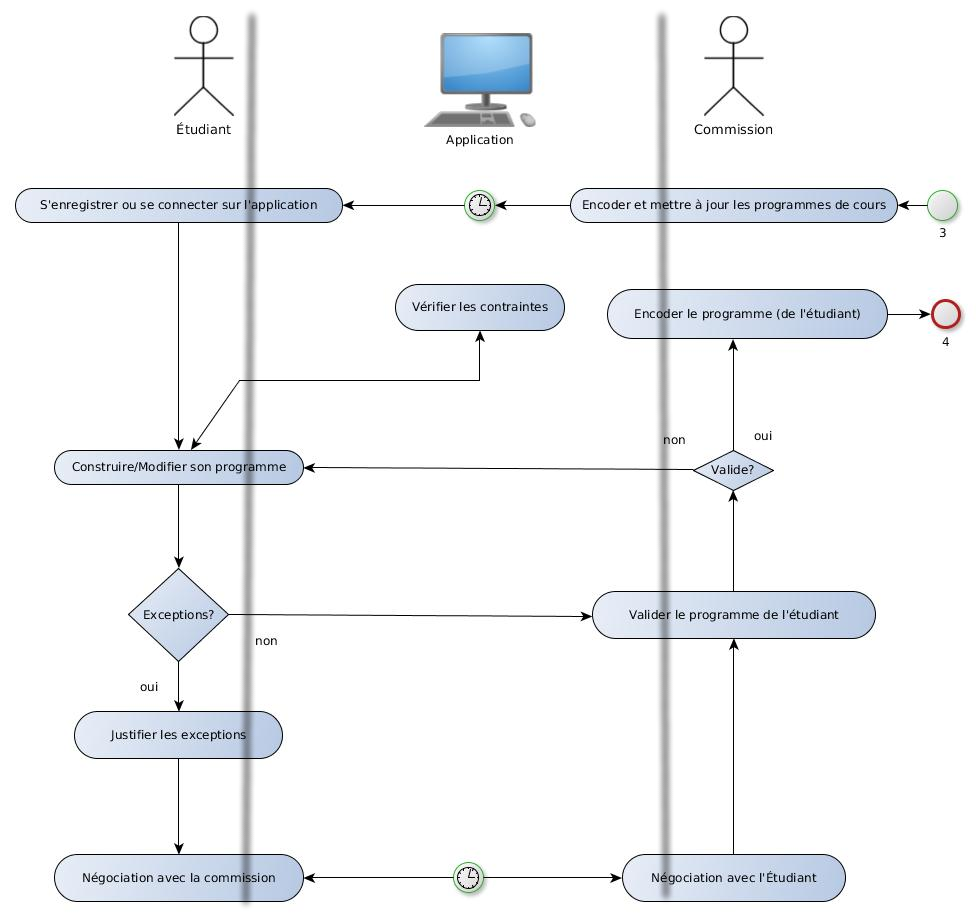
\includegraphics[width=\textwidth]{desired_process}
\end{figure}


La \textit{commission de programme} importe et met à jour les différents programmes à l'aide d'un fichier yEd ou Excel externe qui est ensuite importé dans l'application

L'étudiant se connecte à l'application, crée son programme de cours, et le configure pas à pas en réduisant au maximum le nombre de contraintes non vérifiées. Pour les contraintes non vérifiées restantes, il insère en commentaire les justifications à ces exceptions. 

L'étudiant envoie son programme à la validation. 

\textbf{Négociation} - La \textit{commission de programme} récupère la requête de validation. L'application lui montre les contraintes qui ne sont pas respectées. La \textit{commission de programme} regarde ensuite les justifications de l'étudiant. Si elles ne sont pas suffisantes, la \textit{commission INFO} refuse la demande de validation et commente sa validation en expliquant pourquoi certaines justifications ne sont pas suffisantes. 

Le processus de négociation se répète jusqu'à ce que le programme de l'étudiant soit valide. S'il n'y a pas d'exceptions, l'application peut immédiatement vérifier si le programme de l'étudiant est valide et le valider (si c'est le cas) ou demander de modifier son programme (s'il n'est pas valide).






\chapter{Énoncé du problème}
\label{ennonce}
\lhead{Chapitre 2 - Énoncé du problème}
La gestion des programme de cours n'est pas une chose aisée. La situation est complexe essentiellement pour deux raisons.
\begin{enumerate}
\item La \textit{commission INFO} s'occupe d'un nombre assez élevé de programmes;
\item il existe des contraintes de différentes sortes qui restreignent les étudiants dans les choix qu'ils peuvent faire lorsqu'ils configurent leur programme de cour;
\item les programmes évoluent souvent.
\end{enumerate}

Ces trois points vont être présentés en détail dans les sections qui suivent. 


\section{Programmes proposés}
La liste des programmes proposés par la \textit{commission INFO} est la suivante:


\textbf{Bachelier en sciences informatiques - SINF1BA} \cite{SINF1BA} - C'est un programme de 180 crédits. Comme dans tout programme de bachelier à l'UCL, l'étudiant est amené à devoir choisir une mineure dans ce programme. Par exemple, une mineure intitulée \textit{Approfondissement en sciences informatiques} est disponible pour les étudiants qui suivent ce programme. La durée normale de ce programme de bachelier est de trois ans. 

\textbf{Bachelier en sciences de l'ingénieur, orientation ingénieur civil - FSA1BA (Majeure ou Mineure en informatique)} - \cite{FSA1BA}. Ici il n'est pas question du programme FSA1BA dans son entièreté mais de la majeure ou mineure que l'étudiant en sciences de l'ingénieur est amené à choisir lorsqu'il suit ce programme.

\textbf{Master [120] en sciences informatiques - SINF2M} \cite{SINF2M} - Ce programme de 120 crédits est destiné aux étudiants en provenance du programme \textit{SINF1BA}. Il comporte un module obligatoire (le tronc commun) et la possibilité de choisir un ou plusieurs modules optionnels (Génie logiciel, systèmes de programmation, intelligence artificielle, réseaux et sécurité). La charge du travail de fin d'étude est de 28 crédits. La durée normale de ce programme de master est de deux ans.

\textbf{Master [60] en sciences informatiques - SINF2M1} \cite{SINF2M1} - Ce programme alternatif de 60 crédits est destiné aux étudiants en provenance du programme \textit{SINF1BA}. Il comporte un module obligatoire (le tronc commun) et la possibilité de choisir quelques cours au choix mais pas d'options. La charge du travail de fin d'étude est plus petite que celle de son homologue  \textit{SINF2M}: 18 crédits. La durée normale de ce programme de master est d'un an. 

\textbf{Master [120] : ingénieur civil en informatique - INFO2M} \cite{INFO2M} - Ce programme est destiné aux étudiants en provenance du programme \textit{FSA1BA} ayant suivi soit la mineure soit la majeure en informatique. Comme dans le master \textit{SINF2M}, il comporte un module obligatoire (le tronc commun) ainsi que la possibilité de choisir un ou plusieurs modules optionnels (Génie logiciel, systèmes de programmation, intelligence artificielle, réseaux et sécurité). La charge du travail de fin d'étude est de 28 crédits. La durée de ce programme de master est de deux ans.  

\textbf{Année d'études préparatoire au master en sciences informatiques - SINF1PM} \cite{SINF1PM} - Ce programme est destiné aux étudiants en provenance de Hautes écoles d'informatique. Il permet d'accéder aux programmes \textit{SINF2M} et \textit{SINF2M1}. C'est un programme \textit{à la carte} qui dépend du \textit{background} de l'étudiant (Dans la plupart des cas, c'est un programme standard qui est proposé). Les cours sont choisis parmi ceux proposés dans le programme \textit{SINF1BA}. Ce programme affiche entre 46 et 60 crédits. La durée normale de ce programme est d'un an.  
 

Outre ces programmes, \textit{la commission INFO} doit s'occuper du cas des étudiants en programme d'échange. La principale difficulté, que cela soit un étudiant immigrant ou émigrant, est de trouver des équivalences entre les cours suivis dans l'université d'origine et ceux proposés à l'UCL ou l'inverse. 

De plus, les intersections entre ces cours sont nombreuses. Beaucoup de cours sont disponibles pour une partie voir la totalité des programmes cités ci-dessus.  
\clearpage
\section{Contraintes}
\label{contraintes_intro}

Les contraintes sont un point important du problème. En plus d'être nombreuses et diversifiées, elles requièrent beaucoup de travail au niveau de leur vérification du coté de \textit{la commission INFO}. En outre, elles sont difficiles à exprimer (et vérifier) avec les moyens (formulaire excel, présentation en début d'année, portail du département) mis à la disposition de l'équipe. La conséquence directe de ceci est qu'il est difficile pour les étudiants de comprendre le pourquoi du comment de ces contraintes. Ils n'en tiennent donc pas compte à 100\% lorsqu'ils construisent leur programme de cours.

Voici une liste qui en présente brièvement les différentes sortes que l'on peut rencontrer.
\begin{enumerate}
\item \textbf{Dépendances entre les différents cours} - Ces contraintes  sont de deux types :
	\begin{enumerate}
	\item Les prérequis : Les prérequis d'un cours sont les cours qu'il faut avoir réussis (dans des années académiques antérieures) afin de pouvoir suivre ce cours 
	\item Les corequis : Les corequis d'un cours sont les cours qu'il faut avoir suivis \textbf{au plus tard} durant la même année académique que ce cours.
	\end{enumerate} 

L'image~\ref{fig:cour_dep} illustre ce type de contrainte. On peut voir que le cours \textit{INGI2365} a pour prérequis le cours \textit{SINF1121} et pour corequis le cours \textit{INGI2261}. Il est donc nécessaire d'avoir \textbf{validé} \textit{SINF1121} ainsi que de suivre (au plus tard) \textbf{durant la même période} le cours \textit{INGI2261} (s'il n'a pas été suivi précédemment) pour avoir accès à \textit{INGI2365}. Ces deux contraintes sont directionnelles! le cours \textit{SINF1121} n'a pas pour corequis le cours \textit{INGI2365}, de même que le cours \textit{INGI2261} n'a pas pour prérequis le cours \textit{INGI2365}. 

Notez que l'arrête qui relie le cours \textit{SINF1121} au cours \textit{INGI2365} est interprétée comme directionnelle dans le logiciel. 

\begin{figure}[H]
\centering
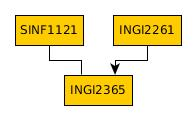
\includegraphics{dependancies_ex}
\caption{Dépendances du cours INGI2261}
\label{fig:cour_dep}
\end{figure}

\item \textbf{Contraintes induites par les programmes} - Ce sont les différents cours ou ensembles de cours qu'il est obligatoire de suivre avant de valider un programme. En master, il y a, par exemple, le module intitulé \textit{Tronc Commun} qu'il est obligatoire de suivre, ainsi que le mémoire. Certains modules optionnels, comme les options de master, sont constitués de sous-modules dont il est obligatoire de suivre la totalité des cours qu'ils contiennent. 

\item \textbf{Contraintes temporelles} - Ce sont les contraintes les plus basiques. Elles représentent la période de temps durant laquelle il est possible de suivre le cours en question. Initialement, elles sont exprimées en terme de semestre. Pour des raisons variables, comme un professeur qui part à la retraite, ou qui prend une année sabbatique, elles peuvent très bien s'exprimer en terme d'années académiques. Un autre exemple sont les cours bisannuels qui sont des cours se donnant une fois tous les deux ans. 

\item \textbf{Contraintes sur les propriétés} - Ces contraintes portent sur les propriétés des cours, programmes ou modules. Principalement, elles portent sur les crédits minimum et maximum d'un programme ou d'un module.

\end{enumerate}


\section{Conclusion}
L'objectif est de développer une application pour que la charge des différents problèmes présentés plus haut (la gestion des contraintes, le nombre des programmes proposés et leur complexité) soit à la charge d'une machine. L'idée est de pouvoir:
\begin{itemize}
\item importer et mettre à jour les données relatives aux catalogues de cours;
\item permettre aux étudiants de conserver un historique des cours et programmes qu'ils ont déjà suivis au cours des années précédentes (et des catalogues d'où proviennent ces cours);
\item visualiser ces données, que l'on soit étudiant ou membre de la commission de programme;
\item effectuer une vérification immédiate de la validité des programmes de cours créés par les étudiants;


\item permettre à la commission de communiquer avec les étudiants via l'application, pour par exemple attirer l'attention de l'étudiant sur une partie de son programme qui ne semble pas cohérente, ou dans l'autre sens, demander ou donner des explications à la commission sur certains points;
\item porter l'application aisément en production (via le \textit{"cloud"} par exemple). 
\end{itemize}

De manière plus générale, le but de ce mémoire est de développer une application conviviale, maintenable et évolutive afin qu'elle puisse être utilisée par les étudiants et la commission de programme. 

Ce mémoire sera typiquement un projet que pourrait rencontrer un informaticien dans la vie active, où la \textit{commission INFO} joue le rôle de client, et le promoteur celui de chef de projet. 
\chapter{Présentation du système}
\label{presentation_systeme}
\lhead{Chapitre 3 - Présentation du système}
\section{Introduction}

Ce chapitre vise, à l'aide d'un exemple concret d'utilisation,  à:
\begin{enumerate}
\item introduire les technologies utilisées pour développer l'application;
\item expliquer les différentes fonctionnalités de l'application d'un point de vue utilisateur. Les utilisateurs étant de deux types, la section relative aux fonctionnalités sera divisées en deux parties. Dans un premier temps, nous expliqueront les fonctionnalités offertes à la commission de programme à savoir;
  \begin{itemize}
    \item l'import de données dans l'application (Programmes de cours, modules, cours);
    \item la gestion des données (Accéder au différents cours, modules et programmes, mettre à jour leurs données);
    \item la gestion des contraintes;
    \item comment vérifier les programmes de cours des étudiants.
  \end{itemize}
Ensuite, nous présenterons ce qu'il est possible de faire en tant qu'étudiant avec l'application à savoir:
\begin{itemize}
  \item se créer un compte utilisateur;
  \item se connecter avec son compte utilisateur;
  \item se créer (ou modifier) un programme de cours, en choisissant le programme à suivre;
  \item configurer son programme de cours, en configurant les différentes années qui le composent et en choisissant les modules de cours à suivre;
  \item vérifier la validité de son programme;
  \item négocier avec la commission de programme la justification des exceptions. 
\end{itemize}
 
\end{enumerate}

Un des principaux objectifs de ce mémoire étant d'offrir une solution maintenable et évolutive, l'application est divisée en trois parties distinctes, indépendantes entre elles. 

Ces trois parties sont les suivantes:
\begin{itemize}
\item l'import et la mise à jour des catalogues, de programmes, modules, cours et des différentes contraintes par la \textit{commission de programme}; 
\item la création du programme par l'étudiant, via l'interface utilisateur;
\item la vérification (par l'application) des différentes contraintes induites par le programme créé précédemment par l'étudiant.
\end{itemize}

\subsection{Exemple d'utilisation}

Tout au long de ce chapitre, l'exemple suivant va être utilisé pour illustrer le fonctionnement de l'application. Il s'agit d'un catalogue de cours fictif proposant deux programmes de cours. Ce programme fictif se rapproche très fort de la réalité. Certaines parties du catalogue (certains modules optionnels du programme de master, certains cours) ont été élaguées pour rendre l'exemple plus clair. L'exemple reste néanmoins représentatif de la réalité, il comporte en effet les différents types de contraintes que l'on peut rencontrer par exemple. 
\begin{figure}
\centering
\caption{Exemple fictif de catalogue de cours}
\label{fig:running_example}
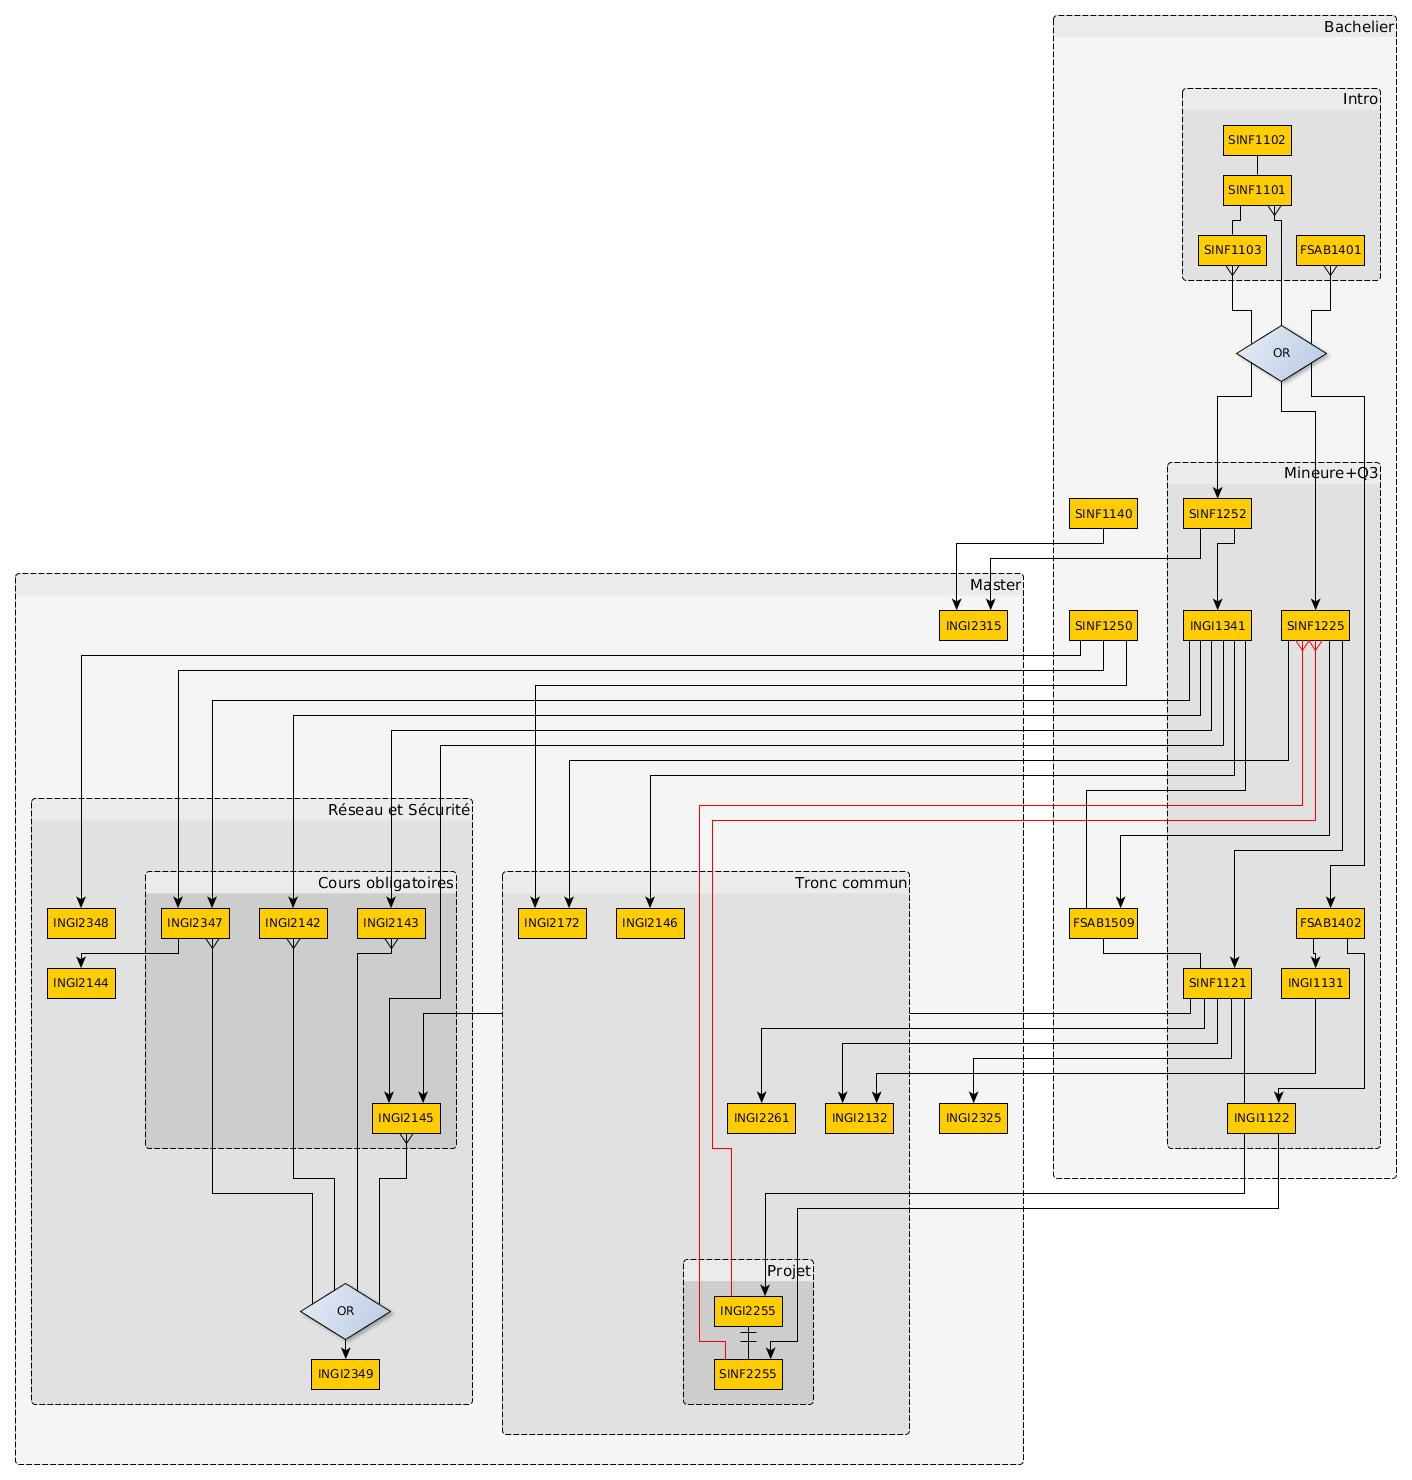
\includegraphics[width=\textwidth]{running_example}
\end{figure}

Ce catalogue est composé de deux programmes de cours.

Un programme de \textbf{Bachelier} (le grand rectangle à droite de la figure \ref{fig:running_example}) composé d'un module obligatoire (Introduction, la petite boite imbriquée s’appelant \textit{Intro})

Un programme de \textbf{Master} (le grand rectangle à gauche de la figure \ref{fig:running_example}) composé d'un module optionnel (l'option réseaux et sécurité, la boite imbriquée à gauche) et d'un module obligatoire (Le tronc commun, la boite imbriquée à droite). De plus, certains cours de master dépendent de cours de bac. 


%************************************************************
\section{Technologies utilisées}
\subsection{Introduction}
Le but poursuivit par cette section est de présenter les différents choix faits aux niveaux des technologies utilisées par l'application. Ces choix sont de deux types. Premièrement, les technologies utilisées pour construire l'application seront présentées, comme le framework ou la base de données qui est utilisée. Les technologies externes à l'application qui sont utilisées pour construire les différents curricula ou mettre à jour leur informations seront présentées par la suite.

On parle de technologie interne pour représenter celles qui sont utilisées pour développer les fonctionnalités de application. Les technologies externes sont quant à elles des applications déjà existantes qu'il faut utiliser \textbf{en dehors} de l'application et pour lesquelles il ne faut pas écrire de lignes de code.
\subsection{Ruby on Rails}
\subsubsection{Introduction}

Cette section a pour but de présenter la technologie principale utilisée pour développer l'application. Le but n'est pas de parcourir en détails le fonctionnement de Rails, mais bien d'en présenter les concepts clés. En effet, il semble important d'en comprendre les grande lignes, car son architecture, aussi bien que ses principes ont influencé la structure de la solution.
\subsubsection{Le choix d'un framework}
A première vue, l'utilisation d'un framework n'est pas absolument nécessaire. Cependant, un framework apporte toute une collection d'outils qui aident à développer mieux et plus rapidement.

\textbf{Mieux} car il permet de développer une application qui est structurée, ce qui rend le code plus maintenable et évolutif.

\textbf{Plus rapide} car il permet de gagner du temps en réutilisant des modules génériques afin de se concentrer sur d'autres domaines. Avec un framework, on assemble des briques plutôt que de réinventer la roue. 

Enfin, le dernier atout d'un framework se situe au niveau de l'intégration de nouveaux développeurs sur le projet. Dans le cadre de ce mémoire, il est clair que de nouvelles fonctionnalités devront être ajoutées dans le futur. De plus, les fonctionnalités existantes devront peut être modifiées ou améliorées. Il sera plus facile pour cette personne de se plonger dans du code qui n'est pas le sien, s'il a une structure propre aux standard web d'aujourd'hui.

\textbf{Il est donc fortement conseillé d'utiliser un framework web pour créer ce genre d'application.} 

Il en existe une multitude aujourd'hui. Il y a tout d'abord les frameworks PHP comme CakePHP, DRUPAL ou Symfony (pour ne citer que les plus connus). Viennent ensuite Ruby on Rails, un framework en ruby et Django, un framework en Python. Cette liste n'est bien entendu pas exhaustive. 
\subsubsection{Le choix de Ruby on Rails}
L'intérêt réside dans le niveau de productivité et de maintenabilité accru que l'on obtient en travaillant avec le framework. Les design patterns sous-jacents, et la philosophie de Rails permettent de concentrer son travail sur les fonctionnalités de l'application plutôt que de passer son temps à écrire du code répétitif ou remplir des fichiers de configuration. 

De plus, il existe une multitude de librairies tierces appelées \textit{ruby-gem} qui réduisent encore le nombre de lignes de code à produire, en apportant des fonctionnalités à l'application. Le meilleur exemple est \textbf{devise}, une librairie qui permet d'ajouter la gestion de l'utilisateur(création, connexion, récupération de mot de passe, envoit de mails, etc ..) en quelques lignes en plus de gérer les sessions et les accès aux différentes actions et vues. 

Rails pousse aux bonnes pratiques, c'est d'ailleurs cette philosophie qui m'a incité à développer la plupart des fonctionnalités, comme vous le verrez plus tard, dans des librairies externes à l'application.


En outre, Rails dispose d'une communauté très active et passionnée, qui teste, documente et améliore les fonctionnalités du framework. 

Les limites du framework sont les suivantes
\begin{itemize}
\item Lorsque l'on débute, on est souvent tenté de charger les modèles en voulant suivre la philosophie \textit{tiny view - skinny controller - fat model}\footnote{Bonne pratique qui consiste à délaisser toute la logique aux modèles} et l'on oublie souvent qu'il est possible de déléguer la plupart des fonctionnalités à des librairies externes, qui sont plus faciles à développer - car crées en pure \textit{ruby} - et plus facile à tester - car indépendantes de rails \cite{fat_models}.

\item Un des principaux aprioris sur les frameworks et particulièrement Ruby on Rails, est qu'il sont lents (et peu efficace). En effet, ruby est un langage interprété . Ce type de langage tend à être plus lent que les langages compilés. Cependant, il faut garder à l'esprit qu'écrire du code, trouver et corriger des bugs ou encore ajouter des nouvelles fonctionnalités dans une application sont des tâches encore plus couteuses en temps. Rails permet de réduire le temps consacré à ces tâches, ce qui est bien plus important lorsque l'on développe ou maintient une application, particulièrement dans le cadre d'un mémoire. Ainsi, à la place de configurer le mapping entre ces différentes ressources, on utilise un convention.
\end{itemize}

\subsubsection{Conclusion}
Pour toute les raisons présentées ci-dessus (libraries externes disponnibles, communauté, etc), le choix s'est naturellement porté vers Ruby on Rails. En outre, j'ai accumulé pas mal d'expérience en utilisant ce framework dans le cadre d'un stage et en réalisant des petits projets ces dernières années. 

C'est un framework open-source, utilisé pour développer des applications web. Le développement se fait à travers le langage de programmation multi-paradigmes (Programmation fonctionnelle, orientée object, ...) \textbf{ruby}. Il se base sur des puissants design patterns et principes qui vont être présentés en quelques lignes ci-dessous.

\subsubsection{DRY - Don't repeat yourself}
Comme son nom l'indique, ce premier principe pousse à la réutilisation du code existant le plus souvent que possible, plutôt que d'avoir des bouts de code similaires un peu partout dans l'application. L'idée de tendre vers une structure \textit{Api}, où tout ce qui n'est pas nécessaire aux classes et méthodes externes est caché en interne. Le principal avantage se situe au niveau de la \textbf{maintenabilité}. On évite ainsi de devoir partir à la recherche des différents bouts de code dupliqués lorsque l'on veut modifier le comportement d'une méthode, d'une classe, ou même d'un module.

\subsubsection{CoC - Convention over Configuration}
L'idée est de réduire au minimum les décisions à prendre avant de commencer à développer. Une convention importante en \textit{Ruby on rails} se situe au niveau des noms des classes pour lesquelles il existe une table correspondante en base de données. Pour un modèle \textit{Course} par exemple, la convention est d'avoir une table nommée \textit{courses} en base de données. Cela permet d'éviter d'avoir à écrire du code supplémentaire pour spécifier à l'application quelle table correspond à quel objet. 

Cela permet au développeur de se concentrer sur les parties non conventionnelles de l'application, comme l'architecture, plutôt que de perdre son temps à configurer les objets. L'avantage ici se situe plus au niveau de la \textbf{productivité}.
\subsubsection{MVC - Model-Vue-Controlleur}

Le framework s'appuie sur le pattern \textbf{MVC}. Destiné aux applications dites \textit{interactives}, il divise l'application en trois parties; le modèle, les vues et le contrôleur. Notez que \textit{Ruby on Rails} ne respecte pas totalement MVC dans sa conception initiale. Cela se justifie par le fait que ce pattern n'est pas destiné à la base aux applications web, notamment car la vue est ici une page web. Le modèle ne peut donc pas lui envoyer tous les changements qui surviennent au niveau des données. C'est la vue, qui doit expressément faire les requêtes pour ces données, à travers le contrôleur.

MVC à la sauce Rails se présente comme suit. Nous avons

\begin{description}
\item[le modèle] lié à une base de données, qui contient les données et l'état de l'application. Il contient aussi tout les objets métiers \footnote{Objets qui font tout le travail.}, qui détermine comment l'information est créée, mise à jour, et affichée;
\item[les vues] qui génèrent l'interface utilisateur et lui présentent les données. Ce composant est passif, il ne traite aucune information. \textit{Vues} est au pluriel ici, car plusieurs vues peuvent avoir accès au même modèle;
\item[le contrôleur] qui reçoit les événements du monde extérieur, interagit avec le modèle et choisit la vue à afficher à l'utilisateur. Par exemple, lorsque l'utilisateur veut éditer un commentaire dans un blog, le contrôleur va rendre la vue relative à l'édition de l'objet correspondant. 
\end{description} 

\subsubsection{Active Record}
Ce pattern quant à lui stocke les données dans une base de données relationnelle. Il s'agit simplement de fournir une abstraction supplémentaire à la base de données et fournir des fonctions pour manipuler les données. Dans le cas de rails, il y a donc une couche ruby entre la base de données proprement dite et la logique dans notre modèle. Cela permet par exemple, d'être indépendant du système de base de données utilisée en dessous.  Par exemple, \textit{postgresql} est le système de gestion de base de données utilisé pour le moment (source : \cite{rails_cast_migration_to_postgresql}. Si pour une raison X ou Y, il devient nécessaire de passer à \textit{sqlite3}, il suffit de changer le fichier de configuration \textit{config/database.yml} de
\begin{lstlisting}
development:
  adapter: postgresql
  database: db/development
  pool: 5
  timeout: 5000
\end{lstlisting}
vers
\begin{lstlisting}
development:
  adapter: sqlite3
  database: db/development
  pool: 5
  timeout: 5000
\end{lstlisting}

Et de recréer la base de données avec
\begin{lstlisting}
rake db:create:all
rake db:migrate
\end{lstlisting}



Tout cela est fait sans devoir changer comment sont accédées les données dans les différents modèles.  

\subsection{Base de données - PostgreSQL}

Rails supporte plusieurs systèmes de gestion de base de données : PostgreSQL, MySQL, SQLite. Le choix du système est cependant restreint à la plateforme utilisée pour héberger l'application (Heroku). En effet, il est nécessaire d'avoir une base de données PostgreSQL pour pouvoir héberger l'application sur Heroku. 

\subsection{Éditeur de graphes - yEd}
\label{yed}
Comme expliqué plus tard dans la section \ref{data_mgmt} détaillant comment sont importés les données, le choix s'est porté vers une importation en deux étapes des données dans l'application. 

\textbf{La première étape} consiste à créer et importer le graphe de cours. Les données importées durant cette étapes sont les nom identifiant les différents objets du graphes (cours, programme, podule), la structure des différents programmes de cours (les cours et modules constituant les programmes de cours) et les dépendances entre les cours.\footnote{Se référer à la section \ref{dependances} (relative aux dépendances) pour plus de détails.}

\textbf{La deuxième étape} consiste à ajouter des nouvelles données des différents objets (ou les mettre à jour) à l'aide d'un formulaire excel. Cela permet d'ajouter des propriétés comme les crédits d'un cours ou les crédits minimum requis d'un programme de cours par exemple.\footnote{Se référer à la section \ref{properties} pour plus de détails.} 

Le but de cette section est d'expliquer les choix qui on été faits aux niveau des technologies utilisées pour s'occuper de \textbf{la première étape} (La construction d'un graphe). 

Pour construire et importer le graphe de cours, plusieurs alternatives se sont présentées.

La première correspond à un logiciel intégré dans l'application, qui permet de construire explicitement un catalogue de cours sous forme de graphe, en proposant exclusivement de placer des objets cours, modules, ou programmes sur le graphe et en n'offrant que des arrêtes de type corequis ou prérequis. Cette application communiquerait directement avec les modèles et permettrait de générer directement les objets (cours, modules, ...) désirés. Cependant il n'existe pas d'applications réalisant ce genre de graphe pour le moment. Il faudrait donc développer un outil, intégré dans l'application,  fournissant ces fonctionnalité. Cependant, cela sort du cadre de ce mémoire, faute de temps. 

La deuxième alternative serait d'intégrer un outil générant des graphes plus standard dans l'application. YWorks offre une solution, yFiles, qui est permet la création et l'édition de graphes en HTML5 et en javascript. Ce logiciel est cependant très chère.

La troisième et dernière alternative serait d'utiliser un logiciel externe à l'application pour générer ces graphes. Ce logiciel, en plus d'être gratuit, doit être multi-plateformes (Mac os x, Linux \& Windows) et capable d'exporter dans un format relativement facile à parser. La liste de ce genre de logiciel est assez longue (Dia, Yed, OmniGraffle, Graphiz)
\begin{itemize}
  \item Dia - C'est un logiciel assez léger qui est capable d'exporter en Xml, un format standard pour représenter des données. Il devient cependant très ennuyeux à utiliser lorsque l'on manipule des graphes de taille importante. C'est cependant un éditeur graphique très générique qui n'est pas seulement destiner à la création de graphes. 
  \item OmniGraffle - Ce logiciel n'est disponible que sur Mac Os X malheureusement.
  \item Yed - Ce logiciel est assez complet. Il est cross-plateforme et à l'avantage de contenir des algorithmes qui permettent de restructurer automatiquement les graphes. Il permet aussi d'exporter en deux formats de types xml (Graphml \& XGml)
  \item (...)
\end{itemize}

Étant donné la contrainte de temps imposé par le cadre du mémoire, le choix s'est porté vers un logiciel déjà existant. Il a été préférable de choisir une solution externe pour éviter de surcharger l'application avec de lourds modules graphiques. De plus, intégrer ce genre de logiciels dans l'application ne changeait rien au fait qu'il fasse parser le fichier exporté par l'outil pour importer les données dans l'application.

YEd a été choisi pour toutes ces raisons. 
\clearpage
%*********************************************************************************************************************************$
\section{Conception}
\subsection{Introduction}
 
L'application est la  plateforme qui tient le rôle d'intermédiaire entre la commission et les étudiants. Elle est représentée par l'entité \textit{Application} sur le diagramme \ref{fig:desired_process_2}. Il y a trois modules attachés à cette entité.

\begin{figure}
\centering
\caption{Processus désiré}
\label{fig:desired_process_2}
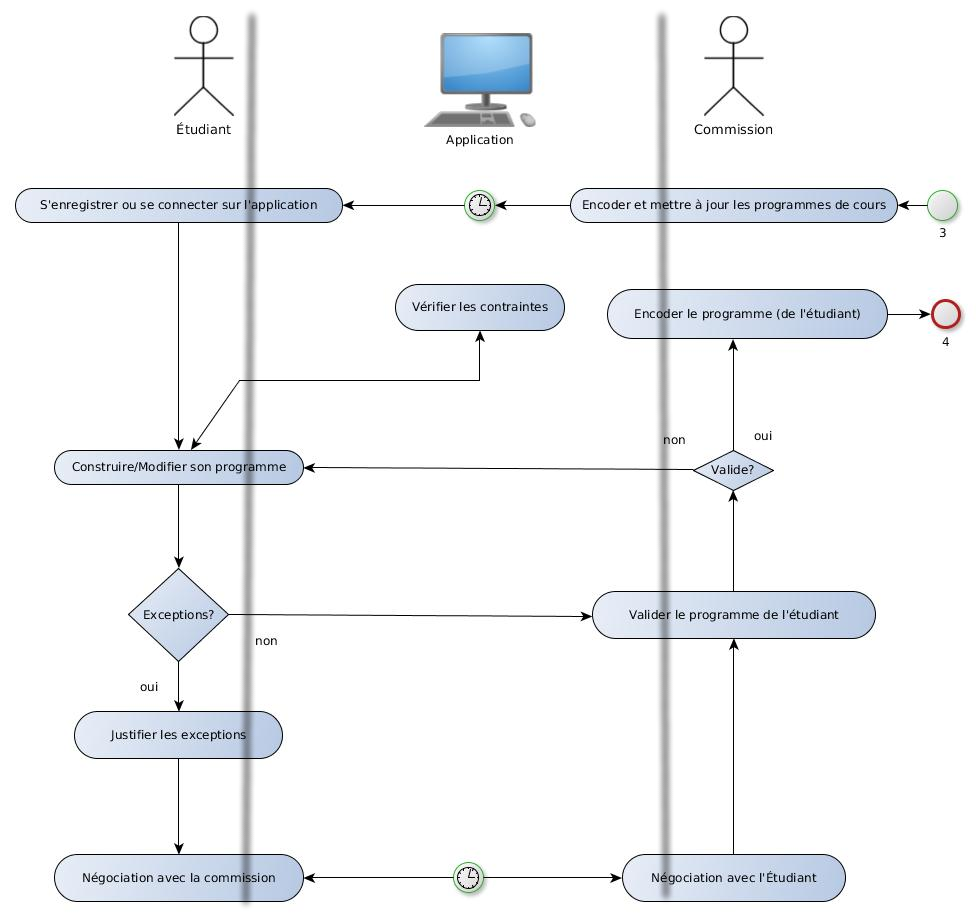
\includegraphics[width=\textwidth]{desired_process}
\end{figure}

\textbf{Le module d'import de données} - Il permet à la commission d'importer les données liées aux curricula  à l'aide de plusieurs supports (qui seront expliqués en détail plus loin dans le chapitre). Ce module permet tout d'abord d'ajouter considérablement plus d'informations dans le support confié à l'étudiant pour qu'il construise son programme. Ensuite, il permet à la commission de mettre à jour facilement ces informations. 
 
\textbf{Le module de gestion des contraintes} - Il vérifie la validité des programmes créés par les étudiants. L'intérêt de ce module est de réduire considérablement  le temps que doit consacrer la commission à la correction des programmes d'étudiants. Premièrement, il contraint les étudiants à justififier les contraintes qui ne sont pas respectées avant d'envoyer leur programme à la validation s'il n'est pas correct. Il fourni aux étudiants un compte-rendu en temps réel de l'état de leurs programmes, en leur pointant les parties qui ne respectent pas les contraintes, quelles contraintes ne sont pas respectées et ce qu'il faut changer dans leur programme pour y remédier.

\textbf{La base de données} - Elle stocke les informations liées aux curricula enregistrés précédemment par la commission, mais aussi les programmes des étudiants. La commission pourra avoir accès aux anciens programmes de cours et à touts les programmes des étudiants. Ces derniers quant à eux, pourront accéder aux différents programmes qu'ils ont déjà suivis et avoir une vision claire de ce qu'il leur reste à valider pour obtenir leur diplôme.

Les fonctionnalités de l'application, telles qu'elles apparaissent sur la figure \ref{fig:desired_process} vont être expliquées dans les sous-sections qui suivent.

\subsubsection{Lexique}
\label{lexique}
Avans de poursuivre l'explication des fonctionnalités de l'application, cette sous-section va expliquer les différents objets qui sont utilisé tout au long de ce chapitre.
\begin{description}
\item[Catalogue] Cet objet est la représentation d'un graphe généré avec yEd une fois importé en base de données. Un catalogue est constitué de plusieurs programmes, modules et cours et est identifié par l'année académique pour laquelle il est destinné. 
\item[Programme] C'est la représentation d'un programme de cours (SINF2M, INFO2M, ...).
\item[Module] C'est un ensemble de cours qui peut être obligatoire (Le tronc comun du programme SINF2M) ou optionnel (les options du programme SINF2M).
\end{description}
\subsection{Gestion des données}
\label{data_mgmt}
Cette section explique comment sont importées les données relatives aux programmes, leurs cours, leurs informations et leurs différentes contraintes. 

Les différentes informations contenues dans chacun des programmes proposés sont les suivantes. Nous avons:
\begin{itemize}
\item plusieurs programmes de cours (SINF1BA, FSA1BA, SINF1PM SINF2M SINF2M1 et INFO2M);
\item chacun de ces programmes contiennent des modules et des cours, avec des informations relatives aux cours et modules obligatoires;
\item chacun de ces cours peut avoir des dépendances \footnote{Se référer à la section \ref{contraintes_intro} et la section \ref{contraintes} pour plus de détails sur ces contraintes};
\item chaque cours, module et programme contient des propriétés. (Le nombre de crédits d'un cours, le semestre durant lequel il est dispensé, l'obligation de suivre un module, le nombre de crédits minium et maximum d'un programme ou module).
\end{itemize}

Il n'est pas viable pour la commission de programme d'ajouter ces informations une à une à l'aide de formulaires permettant d'ajouter et de modifier ces différents objets. Cette approche malgré qu'elle soit facile à mettre en place, contraint la commission de programme à de longues et fastidieuses séances d'encodage de programmes. Qui plus est, chacun des programmes de cours proposés a la forme d'un graphe. La solution la plus logique est donc d'utiliser un éditeur graphique pour construire les différents programme de cours.

La démarche qui a amené à utiliser le logiciel yEd, pour importer la structure des programmes de cours, est expliquée en détail dans la section \ref{yed}. Cette solution a deux conséquences;

\begin{enumerate}
  \item Le logiciel étant externe à l'application, il est nécessaire d'exporter le graphe vers un fichier. Ensuite, il faut parser ce fichier pour en extraire les informations.
  \item On est restreint dans les données que l'on peut ajouter dans un graphe. Ces informations se limitent aux différents labels des nœuds et à leurs dépendances. Une solution est requise pour ajouter les données manquantes. 
\end{enumerate}

Pour \textbf{le premier point}, il a été décidé d'exporter le graphe dans le format \textit{GraphML} (une extension de XML destinée aux graphes). Les informations contenues dans ce fichier sont extraites par l'application à la création du catalogue. Plusieurs formats étaient disponibles pour exporter le graphe créé avec yEd, les raisons qui ont mené à utiliser le format GraphML sont expliquées en détail dans la section \ref{graph_format_justification}.

Les détails de l'implémentation concernant le module qui s'occupe d'extraire les informations contenues dans les graphes sont disponibles dans la section \ref{graph_parsing}.

\textbf{Le deuxième point} justifie le fait que l'importation des données se fait en deux étapes (la première étant l'import du fichier de graphe). Les données manquantes après l'import du graphe sont les suivantes:

\begin{itemize}
  \item les propriétés d'un cours; son sigle (INGI1101 par exemple), le semestre durant lequel il est dispensé, le nombre de crédits, le fait qu'il soit obligatoire;
  \item les propriétés d'un module; son nom, le nombre de crédits minimum et maximum requis pour le valider;
  \item les propriétés d'un programme de cours; son nom, le nombre de crédits minimum et maximum requis pour le valider.
\end{itemize}

La liste de ces propriétés n'est pas exhaustive. Il se peut qu'à l'avenir, le besoin se fasse sentir d'ajouter des informations comme le nom d'un professeur, l'URL du cours, ou toute autre information nécessaire pour des contraintes qui n'ont pas été prévue lors de la conception de l'application. C'est pourquoi en plus de pouvoir d'ajouter et mettre à jour ces informations, il doit être possible d'ajouter des nouvelles propriétés.

Excel a été choisi pour ajouter toutes ces informations car:
\begin{itemize}
  \item il est disponible sur toutes les plateformes (Mac OS, Windows, Linux);
  \item il est facile d'utilisation;
  \item il permet de gérer des grandes quantités d'information de façon structurée;
  \item le format vers lequel il exporte est très facile à parser (XLS)
\end{itemize}

\subsubsection{Conclusion}
L'import de toutes les données se fait en deux étapes. La première consiste à importer le graphe de cours, contenant le nom de chacun des cours, modules et programmes, en plus de leur structure (les cours et modules inclus dans chaque module et programme) et des dépendances entre les cours. Ces informations ne sont pas modifiables une fois le catalogue de cours créé. En cas d'erreure, il n'est pas possible (pour le moment) de mettre à jour les données en téléchargant une nouvelle version du graphe de cours. Il faut donc supprimer le catalogue de cours puis le recréer avec la nouvelle version du graphe.

Les explications relatives aux conventions à utiliser lorsque l'on crée un graphe avec yEd sont disponnibles dans le manuel en annexe.  

La deuxième étape quant à elle, consiste à importer le reste des données dans l'application, via un formulaire excel. Cette étape est répétable, à tout moment les données peuvent être mises à jour sans mettre en péril le fonctionnement de l'application. De plus, il n'y a pas de limites aux informations que l'on peut ajouter de cette manière dans le sens où l'on pourrait rajouter tout et n'importe quoi comme informations (pour peu que l'on vérifie les conventions d'import de formulaire excel) sans faire crasher l'application. 

Cependant, on pourrait, en procédant de la sorte ajouter des incohérences, surtout si l'on modifie les informations relatives aux contraintes. Par exemple, si on ajoute un minimum de crédits à un module qui est plus grand que le maximum de crédits du programme dans lequel il se trouve, il serait impossible pour un étudiant de créer un programme valide.


Les explications relatives aux convetions à utiliser lorsque l'on complète le formulaire Excel sont disponnibles dans le manuel en annexe. 

Par souci de modularité, ces deux étapes sont implémentées dans des modules externes à l'application, comme expliqué dans le chapitre relatif au développement du système \ref{developpement_system}. L'application est relativement indépendante de ces modules, dans le sens ou il serait relativement aisé d'ajouter une méthode encore plus pratique pour ajouter toutes ces informations, sans devoir modifier tout le reste de l'application. Par exemple, on pourrait ajouter manuellement sans passer par ces deux étapes; il suffirait d'implémenter les vues (formulaires de création) correspondantes dans l'application. 




\subsection{Contraintes}
\label{contraintes}
Comme présenté dans la section précédente \ref{contraintes_intro}, les contraintes sont de plusieurs types. Le but de cette section est de présenter les choix que cette catégorisation impose de faire au niveau de la conception des fonctionnalités et d'expliquer plus en détails la logique intrinsèque des plus compliquées d'entre elles.    

Comme expliqué dans les sections qui suivent, la location des informations relatives aux contraintes (les crédits et les dépendances d'un cours par exemple) n'est pas la même pour toutes les contraintes. Qui plus est, chaque contrainte n'est pas vérifiée de la même façon. Une dépendance par exemple implique d'aller chercher si un cours est présent dans un programme, alors que le minimum de crédits requis d'un programme implique de compter les crédits de chacun ces cours. Enfin, chaque contrainte ne renvoie pas les même informations lorsqu'elle n'est pas valide (il faut renvoyer le cours le type de dépendance et le cours lié à la dépendance lorsqu'elle n'est pas valide par exemple). 

 
Dès lors, pour ne pas surcharger les modèles de l'application et la rendre plus flexible (et ainsi conserver un faible couplage et une haute cohésion), la vérification de ces contraintes a été déléguée à un module externe. On évite, ainsi, de se retrouver avec des modèles dont la taille se chiffre en milliers de lignes de code qui sont très difficile à maintenir et faire évoluer. 
\subsubsection{Dépendances}
\label{dependances}
Comme expliqué précédemment les dépendances peuvent être des prérequis ou des corequis. En plus de cela, ces contraintes peuvent être:
\begin{description}
\item[binaires]; elles concernent deux cours; un cours \textit{source} et un cours \textit{destination}; le sens de la contrainte étant celui de la flèche (le cours source est le prérequis du cours destination par exemple);
\item[n-aire]; elles sont composées de plusieurs cours \textit{sources} et de plusieurs cours \textit{destinations}.
\end{description}
 
Pour chaque ensemble n-aire de dépendances, il existe une condition qui s'applique sur chacune des dépendances qui le constitue. Cette condition est soit une disjonction (OR), soit une disjonction exclusive (XOR). L'effet de la condition est la suivante. Il n'y a pas de représentation explicite pour les conjonctions de dépendances car elle peuvent être représentées simplement par des relations binaires.

\begin{itemize}
\item Une contrainte disjonctive ne sera valide que s'il existe au moins une des sous-contraintes qui est vraie.
\item Une contrainte disjonctive exclusive ne sera valide que s'il n'existe qu'une et une seule des sous-contraintes qui est vraie.
\end{itemize}

Il y a un exemple de chaque cas qui se trouve dans l'exemple fictif \ref{fig:running_example}. La contrainte disjonctive se trouve dans le programme de Bachelier. La contrainte disjonctive exclusive quant à elle se trouve dans l'option Réseau et Sécurité du programme de Master.

\begin{figure}
\centering
\caption{Contrainte n-aire disjonctive}
\label{fig:nary_or_constraint}
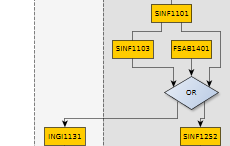
\includegraphics[scale = 0.7]{nary_or_constraint}
\end{figure}


Sur l'image \ref{fig:nary_or_constraint} apparait en détail la contrainte disjonctive;
\begin{itemize}
  \item \textit{SINF1252} et \textit{INGI1131} sont les cours \textit{destinations}
  \item \textit{SINF1101} \textit{SINF1103} et \textit{FSAB1401} sont les cours \textit{sources}
\end{itemize}

Ces contraintes étant des prérequis, il est donc nécessaire d'avoir suivi et réussi \textit{SINF1103} \textbf{OU} (OR) \textit{SINF1101} \textbf{OU}(OR) \textit{FSAB1401} pour pouvoir suivre \textit{SINF1252} \textbf{OU}(OR) \textit{INGI1131}

Sur l'image \ref{fig:nary_xor_constraint} apparait en détail une contrainte disjonctive exclusive;

\begin{itemize}
\item \textit{INGI2349} est le cours \textit{destination};
\item \textit{INGI2145}, \textit{INGI2142}, \textit{INGI2143} et \textit{INGI2347} sont les cours sources.
\end{itemize}

Ces contraintes étant des corequis, il est donc nécessaire d'avoir suivit au plus tard la même année un et un seul des cours \textit{sources} pour pouvoir suivre le cours \textit{INGI2349}. Si l'on suit deux, trois ou la totalité des cours \textit{sources}, la contrainte en sera pas valide!

\begin{figure}
\centering
\caption{Contrainte n-aire disjonctive exclusive}
\label{fig:nary_xor_constraint}
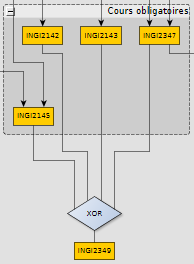
\includegraphics[scale=0.7]{nary_xor_constraint}
\end{figure}

Notez que les dépendances sont importées à l'aide du logiciel yEd \ref{yed}. Il n'est donc pas possible de les modifier, pour le moment, une fois le graphe importé dans l'application. Dans l'état actuel des choses, si l'on désire modifier la structure d'un catalogue de cours (çàd sont graphe), il faut recréer le catalogue de cours avec le graphe modifié. Nous perdons cependant toute les informations additionnelles ajoutées via l'import de formulaires Excel. La mise à jour de la structure d'un catalogue de cours est une des améliorations à apporter à l'application, comme présenté dans le chapitre \ref{futur_work} relatif aux travaux futurs.
\subsubsection{Contraintes s’exerçant sur les propriétés des cours, modules et programmes}
\label{properties}
Ces contraintes regroupent plusieurs catégories de contraintes au sens où elles on été présentées dans le chapitre \ref{contraintes_intro}. On dit que ces contraintes portent sur des propriétés car leur validité dépend de l'information contenue dans celles-ci. Pour reprendre l'exemple du minimum de crédits requis pour valider un programme de cours. La validité de cette contrainte dépend (en plus des cours et modules qui composent ce programme) de deux choses:
\begin{enumerate}
  \item la valeur de cette propriété MIN, contenue dans la propriété du même nom de l'objet Programme;
  \item la valeur de la propriété CREDITS qui compose chacun de ses cours
\end{enumerate}

Par exemple, si le module \textit{Réseau et Sécurité} de l'exemple \ref{fig:running_example} comporte la propriété \textit{MIN, 15}, la méthode qui vérifie les contraintes sur les propriétés de type \textbf{MIN} va aller compter un à un les crédits de chacun des cours qui compose le module, ainsi que chacun des cours qui composent chacun de ses sous-modules (le module intitulé \textit{Cours obligatoires} ici).

Le module de contraintes n'a pas la charge de vérifier tous les types de contraintes. Dans le cas de la contrainte temporelle sur les semestres (qui implique qu'un cours doit être suivit durant le semestre au cours duquel il est dispensé), la vérification est implicite. En effet, la configuration de chaque année se faisant par semestre, il n'est pas possible pour un étudiant de choisir un cours, pour un semestre donné, qui n'est pas dispensé pendant ce semestre. 

Les données relatives à ces propriétés sont importées et mises à jour par le module qui s'occupe d'importer les formulaires Excel. Elle peuvent donc être, contrairement aux dépendances, modifiées quand on le souhaite.  


%*****************************************************
\clearpage
\subsection{Fonctionnalités de l'application - Commission de programme}
\subsubsection{Introduction}
 Une fois connecté à l'aide du compte admin, nous arrivons à la page illustrée sur la figure suivante \ref{fig:landing_page_admin}. Quatre menus sont accessibles depuis la barre de navigation (en haut dans la page d’accueil):
 \begin{description}
  \item [Catalogue] Ce menu offre l'accès à la gestion des catalogues. C'est ici que les catalogues sont importés (via le graph yEd) et mis à jour (via le formulaire Excel). Ce menu permet aussi de gérer les versions des catalogues, pour permettre de mentionner quel est le catalogue principal (celui qui sera utilisé par défaut par les étudiants), quels sont les anciens catalogues (Pour permettre aux étudiants d'avoir accès aux anciens programmes de cours) et quels sont les futurs catalogues qui, toujours en construction, ne sont pas accessibles aux étudiants. 
  \item [Demandes de validation] Ce menu offre l'accès aux requêtes de validation envoyées par les étudiants. La commission de programme aura accès ici au programme d'étudiant lié à la demande de validation, à l'état de celui-ci (est il valide?) et à ses justifications en cas de contraintes non vérifiées dans son programme. C'est ici que la commission de programme accepte ou refuse les programmes d'étudiants.
  \item [Gérer les années] Ce menu offre la possibilité à la commission de marquer les années comme réussies ou ratées (en choisissant les cours réussis). 
  \item [Discussions] Ce menu permet d'accéder aux différentes discussions qui apparaissent lors du processus de négociation entre la commission de programme et les étudiants, lorsque ces derniers sont amenés à justifier les exceptions éventuelles qui surviennent dans leur programme de cours. 
  \end{description}
\begin{figure}
\caption{Page d’accueil}
\label{fig:landing_page_admin}
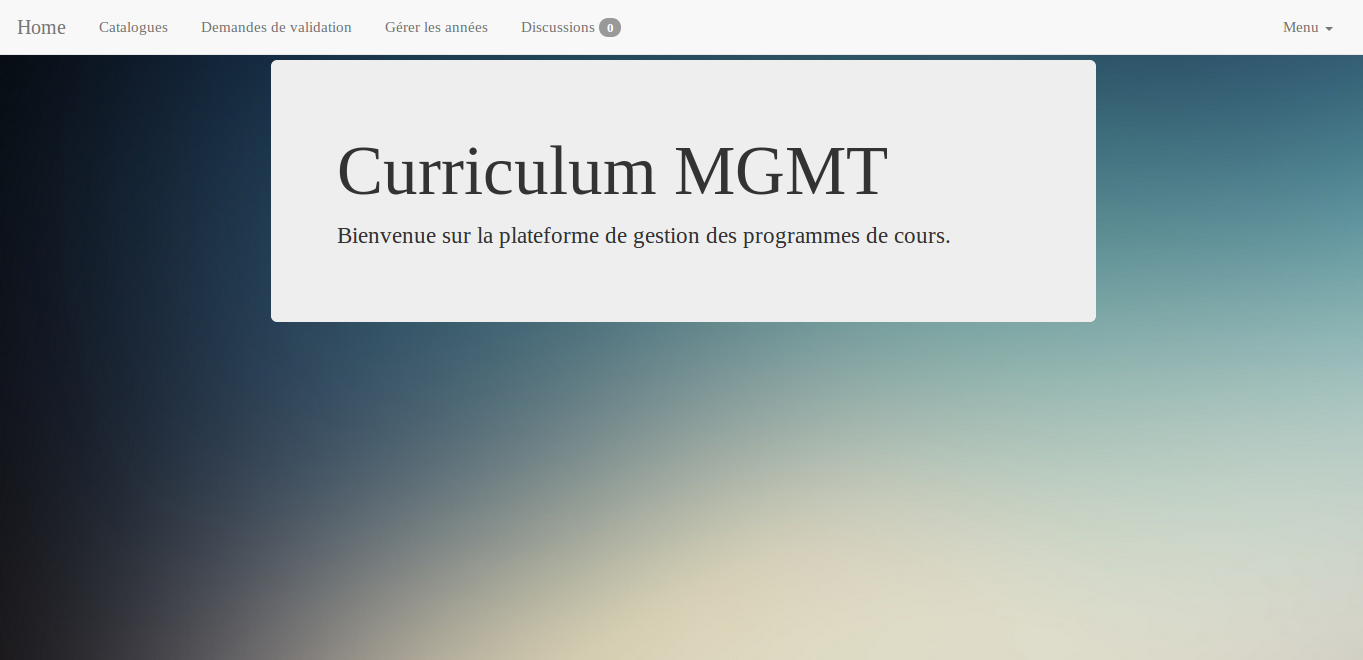
\includegraphics[width=\textwidth]{landing_page_admin}
\end{figure}

%**********************************************
\subsubsection{Encoder et mettre à jour les programmes de cours}
L'ajout de nouveaux programmes de cours se fait en deux étapes dans l'application (comme expliqué dans la section \ref{yed}). La première étape correspond à l'import du graphe créé avec yEd. Cette étape importe dans la base de données les différents programmes de cours, leurs modules, leurs cours et les dépendances entre ces cours.

Cependant, les informations ajoutées par l'intermédiaire de cette étape ne sont pas suffisantes. Il manque toutes les propriétés des différents objets qui, en plus d'être des compléments d'information, servent pour certaines contraintes comme expliqué dans la section précédente \ref{contraintes}. C'est pourquoi il existe une deuxième étape qui permet d'importer un formulaire Excel contenant les informations complémentaires des différents cours, modules et programmes (le nombre de crédits minium et maximum d'un programme, le nombre de crédits d'un cours, le semestre durant lequel il est dispensé). 


Reprenons  l'exemple \ref{fig:running_example}. Les différents programmes de cours sont importés dans l'application par l'intermédiaire d'un module important les graphes yEd. Un catalogue de cours représente l'ensemble des programmes de cours présent sur le graphe \ref{fig:running_example}. Le formulaire suivant \ref{fig:catalog_new_page} permet de créer ces catalogues. 

\begin{figure}
\centering
\caption{Création d'un nouveau catalogue de cours}
\label{fig:catalog_new_page}
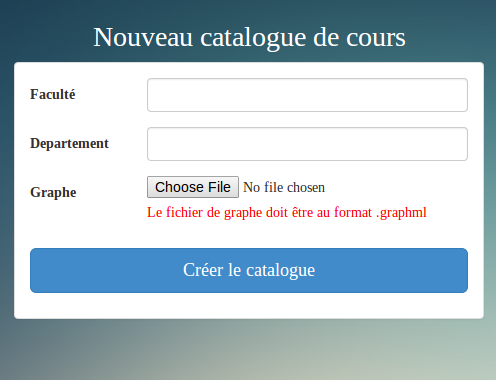
\includegraphics[width=\textwidth]{catalog_new}
\end{figure}


L'utilisateur peut choisir l'année académique et le nom qui vont identifier le catalogue de cours. Cette différenciation est importante car l'application gère plusieurs version de catalogues. Ces versions sont de trois types: 

\begin{enumerate}
\item la version principale; cette version correspond au catalogue qui sera utilisé par défaut par les étudiants. Il ne peut avoir qu'un seul catalogue principal dans l'application. Lorsqu'un étudiant crée un compte utilisateur, il suit par défaut le catalogue principal. Un utilisateur peut cependant choisir un autre catalogue parmi les version anciennes. 
\item les anciennes versions; ces versions correspondent aux anciens catalogues principaux; à chaque fois qu'un catalogue est élu ``principal'', la version du catalogue principal devient ancienne; il n'y a pas de limites sur le nombre de catalogues anciens;
\item les version futures; ces versions correspondent aux nouveaux catalogues créés par la commission de programmes, qui ne sont pas encore disponibles aux étudiants; il n'y a pas de limites sur le nombre de catalogues futurs et ils ne sont pas accessibles aux étudiants. 
\end{enumerate}

\label{catalog_version}
La version d'un catalogue de cours évolue comme suit. À sa création il a la version \textit{future}. Ensuite il passe à la version \textit{principale} lorsque la commission le décide. Enfin, il passe à la version \textit{ancienne} lorsqu'un autre catalogue est \textit{élu} \textit{principal}. 

L'ajout, la modification et la récupération des informations relatives aux cours, modules et programmes se fait par l'intermédiaire d'un module d'import de fichiers Excel. Les consignes pour présenter les données sont expliquées en détails dans le manuel présent en annexe. Pour plus de facilité, il est possible de télécharger directement un template de ce formulaire depuis l'application. La structure reconnue par le module d'import est présente dans ce template, ainsi que le nom des différents cours, modules et programmes présents dans la base de données. De plus, il y a aussi, pour chaque type d'objet (cours, modules et programmes) des exemples de propriété. 

Reprenons l'exemple fictif illustré sur l'image \ref{fig:running_example}. Lorsque l'on crée un catalogue avec ce graphe, et que l'on télécharge juste après le formulaire Excel, on obtient les informations suivantes.

\begin{itemize}

\item Sur la page des programmes (Figure \ref{fig:excel_programs_ex}), les propriété relatives aux nombres minimum et maximum (MIN et MAX) de crédits d'un programme sont proposées.

\item Sur la page des modules (Figure \ref{fig:excel_modules_ex}), les propriétés relatives aux nombres minimum et maximum (MIN et MAX) de crédits d'un module sont proposées. De plus, on peut aussi spécifier si le module est obligatoire ou non.

\item Sur la page des cours (Figure \ref{fig:excel_courses_ex}), les propriétés relatives au semestre durant lequel le cours est dispensé sont notamment proposée, ainsi que la propriété \textit{obligatoire} d'un cours. 

\end{itemize}

La liste de ces propriétés n'est pas exhaustive. En effet il suffit, pour rajouter une nouvelle propriété, de simplement l'ajouter dans le formulaire. Le module d'import de données se chargera de créer les propriétés correspondantes si elles ne sont pas vide dans le formulaire. 

Pour afficher les nouvelles propriétés, il suffit de les afficher dans la vue correspondante (se rendre dans la page cours\#show et récupérer l'information de la nouvelle propriété par exemple)

Pour ajouter une contrainte sur une nouvelle propriété il faut;
\begin{itemize}
\item ajouter la classe correspondante dans le module de contraintes;
\item créer l'objet de cette classe dans le modèle correspondant;
\item traiter les informations (de la nouvelle contrainte) renvoyées par le module de contraintes;
\end{itemize}

Les détails d'implémentation des nouvelles contraintes sont expliquées dans la section \ref{constraint_mgmt}. 

\begin{figure}
\centering
\caption{La page relative aux programme d'un template de formulaire}
\label{fig:excel_programs_ex}
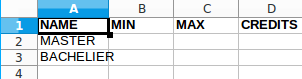
\includegraphics[width=\textwidth]{excel_programs_ex}
\end{figure}

\begin{figure}
\centering
\caption{La page relative aux cours d'un template de formulaire}
\label{fig:excel_courses_ex}
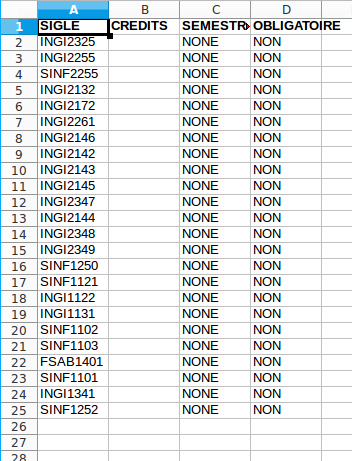
\includegraphics[width=\textwidth]{excel_courses_ex}
\end{figure}

\begin{figure}
\centering
\caption{La page relative aux modules d'un template de formulaire}
\label{fig:excel_modules_ex}
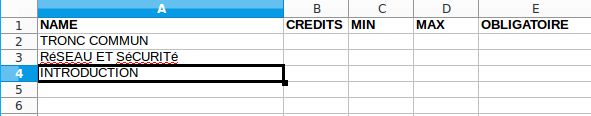
\includegraphics[width=\textwidth]{excel_modules_ex}
\end{figure}

\begin{figure}[!htb]
\centering
\caption{Un catalogue de cours après sa création}
\label{fig:catalog_show}
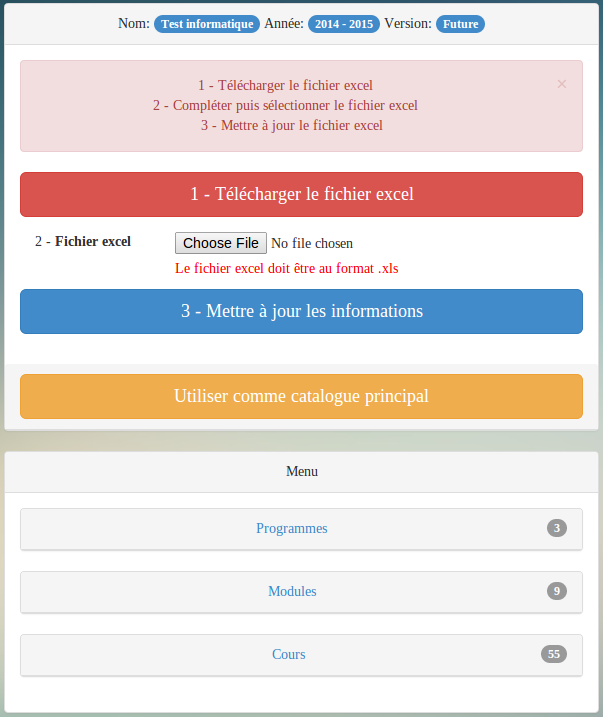
\includegraphics[width=\textwidth]{catalog_show}
\end{figure}

Toutes ces fonctionnalités sont accessibles depuis la page telle qu'elle est illustrée sur l'image \ref{fig:catalog_show}. Le menu déroulant du bas permet d'accéder aux différents programmes, modules et cours du catalogue (le tout, sans devoir recharger la page). En haut à gauche apparaissent les trois propriétés identifiant notre catalogue, à savoir son nom, son année académique et sa version. 

En naviguant dans les différents sous-menus du catalogue (cours, programmes, modules), vous pouvez accéder aux informations complètes concernant ces objets. Il est possible par exemple d'accéder aux détails des contraintes d'un cours. Il est notamment possible de créer des programmes de cours \textit{customisés} à partir des informations présentes dans le catalogue (cours, modules). On pourrait donc par exemple créer un programme \textit{Erasmus} ou \textit{Mercator} avec les modules et cours disponibles, pour proposer aux étudiants étrangers un programme de cours adapté à leur profil.

%***********************************************
\subsubsection{Gérer les années des étudiants}
\label{year_mgmt}
Bien qu'elle ne soit pas mentionnée sur le diagramme \ref{fig:desired_process}, la fonctionnalité qui permet à la commission de programme de marquer les années des étudiants comme réussie, ou comme ratée (en sélectionnant les cours réussis) est relativement importante pour le bon fonctionnement du module qui s'occupe de vérifier les contraintes. 


En effet, pour vérifier la validité des contraintes de type \textit{dépendance} (se référer à  la section \ref{dependances} pour plus de détails), il est nécessaire de différencier les années réussies des années ratées, et de différencier, dans ces années ratées, les cours crédités des cours ratés. Ainsi, le module qui vérifie les contraintes ne prendra pas en compte un cours qui est présent dans une année mais qui n'a pas été crédité lorsqu'il vérifiera certaines contraintes. Par exemple, lorsque l'on vérifie si le nombre de crédits minimum d'un module est atteint, ou si le prérequis d'un cours est valide, il ne faut pas prendre en compte les cours qui n'ont pas été crédités. 

Pour les mêmes raisons, il est primordial de garder une trace des années ratées de l'étudiant, pour savoir quels cours l'étudiant a validé durant cette année qu'il n'a pas réussie.

On peut donc gérer sur la page \ref{fig:year_mgmt} les années des étudiants. Marquer une année comme réussie ou ratée empêchera à l'avenir l'étudiant de modifier ou de supprimer son année dans la page de gestion de son programme. Pour marquer son année comme ratée, il suffit de sélectionner les cours ont été crédité (comme on peut le voir sur la figure \ref{fig:failed_year_mgmt})
\begin{figure}[!htb]
\centering
\caption{La page de gestion des années}
\label{fig:year_mgmt}
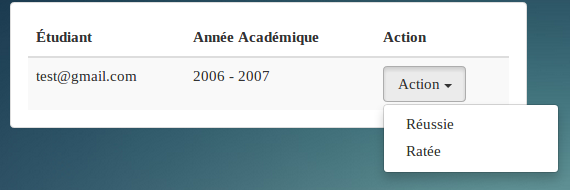
\includegraphics[width=\textwidth]{year_mgmt}
\end{figure}

\begin{figure}
\centering
\caption{Gérer une année ratée}
\label{fig:failed_year_mgmt}
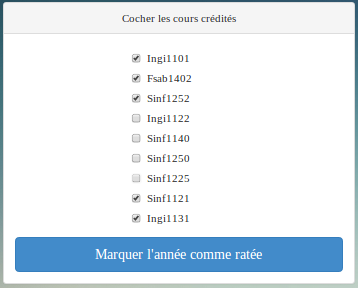
\includegraphics[width=\textwidth]{failed_year_mgmt}
\end{figure}

%********************************************
\subsubsection{Gérer les demandes de validations}
Cette fonctionnalité s'occupe de gérer les étapes \textit{Négociation avec l'étudiant et Valider le programme de l'étudiant} du processus représentée sur le diagramme \ref{fig:desired_process}. 

Lorsqu'un étudiant pense que son programme est correct, il envoie une demande de validation à la commission de programme. Dans le meilleur des mondes, le programme de l'étudiant respecte toutes les contraintes imposées par le programme qu'il suit. Cependant, pour une raison X ou Y, il arrive qu'un étudiant pense avoir une bonne raison pour enfreindre une ou plusieurs contraintes.

Prenons l'exemple d'un étudiant en provenance d'une autre université qui vient suivre un programme de master à l'UCL. En regardant attentivement l'exemple fictif \ref{fig:running_example}, on s’aperçoit que le cours \textit{INGI2315} du programme de master a une dépendance (\textit{SINF1140}) dans le programme de bachelier. Lorsque l'étudiant construit son programme de MASTER, il va se trouver avec des contraintes non respectées qu'il ne sera pas possible pour lui de corriger. 

Comme expliqué dans la section relative aux fonctionnalités offertes à l'étudiant qui suit \ref{validation_request}, l'application permet à l'étudiant, sous certaines conditions (remplir une justification s'il subsiste des contraintes non vérifiées par exemple), de soumettre un programme non valide à la validation. Lorsque notre étudiant soumettra son programme, il remplira un formulaire de justification avant d'envoyer sa demande de validation.

La page qui donne accès à la commission de programme aux demandes de validations est la suivante \ref{fig:validation_mgmt}. Sur cette page, la commission de programme peut accéder aux programmes de l'étudiant (Menu Programme) et accéder à un menu qui permet de voir les contraintes non-vérifiées du programme et leur justification (Menu Exceptions). Ce dernier menu (Justification) permet aussi d'envoyer des message à l'étudiant pour demander des informations supplémentaires.

La page \ref{fig:exception_mgmt} donne accès à la justification du programme d'un étudiant. Dans cet exemple il manque, dans le programme de l'étudiant, plusieurs cours obligatoires. De plus, il a dépassé le maximum autorisé de son programme ainsi que des deux modules qui le compose. Sur cette page, la commission de programme à accès aux détails de chacune des contraintes non respectées du programme de l'étudiant. À droite de chaque contrainte non respectée se trouve la justification de l'étudiant. Comme affiché sur la page \ref{fig:exception_send_message}, la commission a aussi la possibilité d'envoyer un message à l'étudiant pour lui demander des informations supplémentaires. 

Une fois les exceptions vérifiées, la commission n'a plus qu'à valider la demander ou bien la refuser. 




\begin{figure}
\centering
\caption{Page de gestion des demandes de validation}
\label{fig:validation_mgmt}
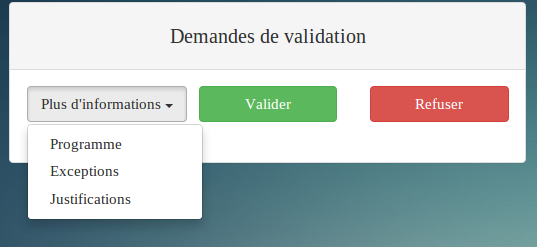
\includegraphics[width=\textwidth]{validation_mgmt}
\end{figure}

\begin{figure}[!htb]
\centering
\caption{Les exceptions d'un programme et leurs justifications}
\label{fig:exception_mgmt}
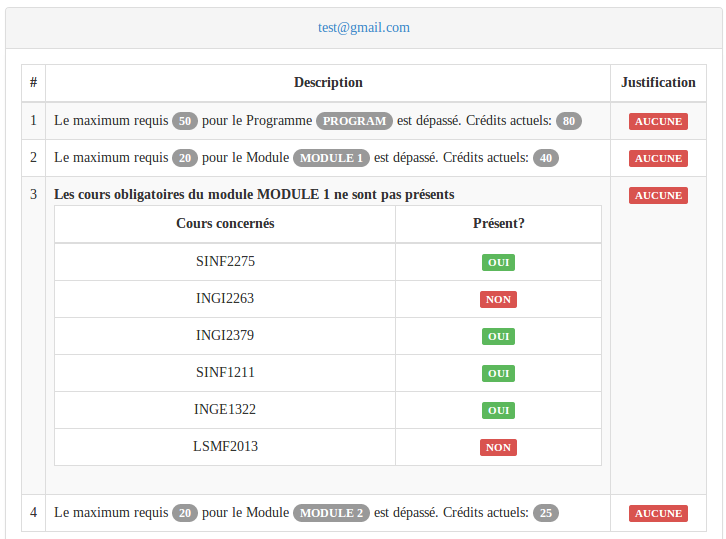
\includegraphics[width=\textwidth]{exception_mgmt}
\end{figure}

\begin{figure}
\centering
\caption{Demander des informations supplémentaires à un étudiant}
\label{fig:exception_send_message}
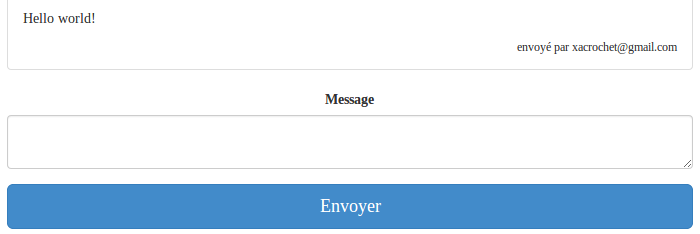
\includegraphics[width=\textwidth]{exception_send_message}
\end{figure}

%*******************************************$$
\clearpage
\subsection{Fonctionnalités de l'application - Étudiant}
\subsubsection{Introduction}
Une fois connecté à l'application, l'étudiant arrive sur la page illustrée sur la figure \ref{fig:student_landing_page}. Deux menus sont accessibles dans la barre de menu en haut; 

\begin{description}
  \item[Mes programmes de cours] Ce menu permet d'accéder à la création du ou des programmes suivis par l'étudiant. C'est par ici que le module de contraintes est appelé pour vérifier la valider des programmes de cours. 
  \item[Programmes disponibles] Ce menu permet d'accéder en détail aux programmes proposés. Il est aussi possible de changer la version du catalogue utilisé via ce menu. (Les différentes versions et leur utilité est expliquée dans la section \ref{catalog_version})
\end{description}
\begin{figure}
\centering
\caption{Page d’accueil des étudiants}
\label{fig:student_landing_page}
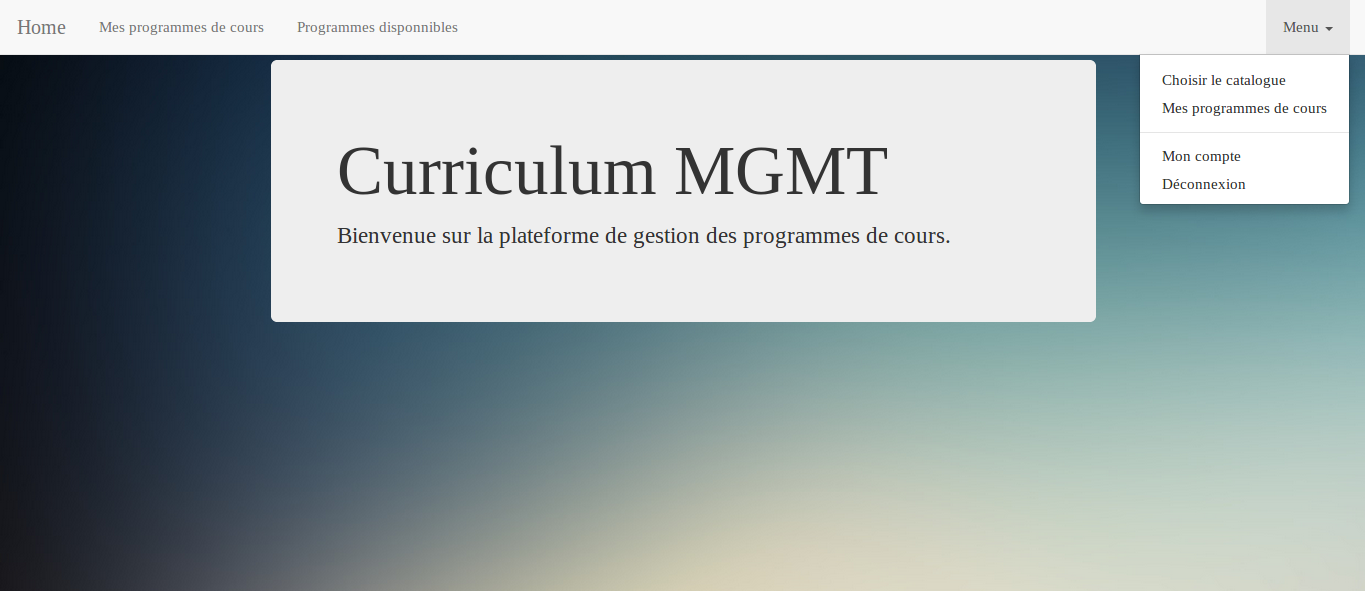
\includegraphics[width=\textwidth]{student_landing_page}
\end{figure}

Les sous-sections suivantes expliqueront les différentes fonctionnalités offertes aux étudiants. 

%********************************************************
\subsubsection{Accéder au programmes de cours disponibles}

Lorsqu'un étudiant désire créer un programme de cours, il doit tout d'abord choisir le programme qu'il va suivre. Si nous reprenons l'exemple fictif \ref{fig:running_example}, il y a deux programmes proposés dans ce catalogue; celui de BACHELIER et celui de MASTER. Comme expliqué dans la section \ref{catalog_version}, plusieurs versions de catalogues de cours sont disponibles dans l'application. 

Pour le moment, il n'est pas possible de rendre un cours disponible dans plusieurs programmes lorsque l'on crée le graphe avec yEd. Cependant, il arrive souvent que cette situation se produise, notamment pour les programmes SINF2M et INFO2M qui ont ne nombreux cours et modules en commun. C'est pourquoi la commission, en attendant qu'une solution plus efficace soit implémentée, doit créer deux catalogues différents. Un étudiant doit donc avoir la possibilité de choisir le catalogue qu'il va suivre en fonction du type de programme dans lequel il se trouve (ingénieur civil ou sciences informatiques).

On peut voir sur l'image \ref{fig:prgrm_availables} les programmes disponibles dans le catalogue de l'exemple fictif. 

\begin{figure}
\centering
\caption{Programmes disponibles}
\label{fig:prgrm_availables}
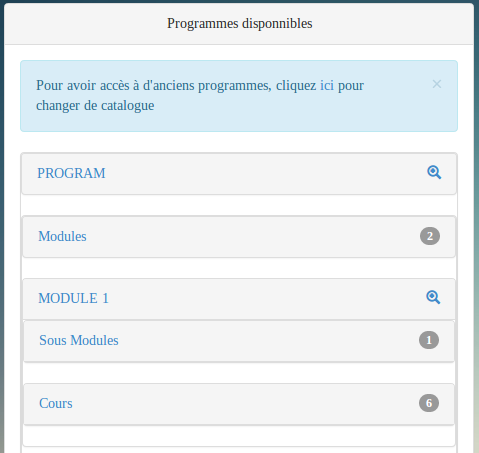
\includegraphics[width=\textwidth]{prgrm_availables}
\end{figure}

%********************************************************
\subsubsection{Configuration d'un programme d'étudiant}
\label{prgrm_mgmt}
Un étudiant à deux choses à faire pour configurer son programme; configurer les différentes années qui le constituent et choisir les différents modules. La page illustrée sur l'image \ref{fig:program_configure} affiche les différentes fonctionnalités à la disposition de l'étudiant. 

Notez que le bouton \textit{Envoyer à la validation} est désactivé pour le moment. En effet, il n'est possible d'envoyer son programme à la validation que lorsque certaines conditions sont remplies, pour éviter que la commission de programme reçoivent des demandes de validations pas assez complètes. Les conditions requises pour pouvoir envoyer son programme à la validation seront expliquées en détail dans la section \ref{fig:validation_mgmt}. 

 
L'idée, pour construire son programme est de configurer chacune des années qui le composent et de choisir les modules correspondant, pour éliminer une à une les contraintes qui ne sont pas respectées. Si nous reprenons le diagramme \ref{fig:desired_process}, l'étape qui correspond à cette section est celle qui s'intitule \textit{Construire/Modifier son programme}.



\begin{figure}
\centering
\caption{Configuration du programme}
\label{fig:program_configure}
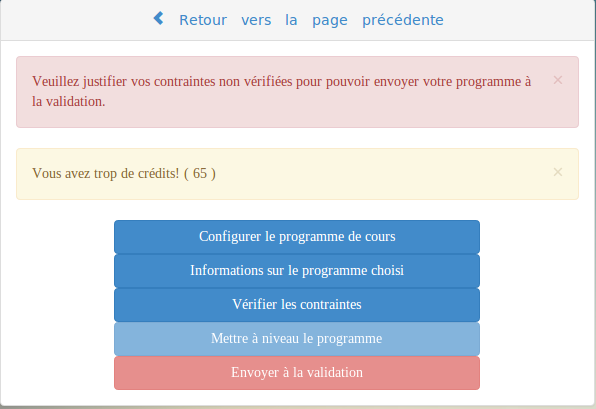
\includegraphics[width=\textwidth]{prgrm_configuration}
\end{figure}

La page \ref{fig:program_configure} permet d'accéder aux différent menus qui permettent de configurer un programme d'étudiant à savoir;
\begin{enumerate}
\item configurer le programme
\item accéder aux informations du programme suivit par l'étudiant
\item vérifier les contraintes et justifier celles qui ne sont pas respectés
\item mettre à niveau le programme si une nouvelle version est émise par la commission de programme
\item envoyer le programme à la validation
\end{enumerate}

La page permettant à l'étudiant de configurer une année de son programme est illustrée sur l'image \ref{fig:year_configuration}. Les cours sont affichés en fonction de leur semestre et de s'il sont obligatoires ou non. Un cours sera obligatoire s'il a été marqué comme tel via le formulaire Excel, ou si son module parent l'est aussi.

Notez que si la commission n'a pas complété les informations après avoir importé le graphe, les champs \textit{SEMESTRE} de chacun des cours ne seront pas initialisés. Aucun de ces cours ne sera affiché dans cette vue, cela, afin de permettre la vérification automatique des contraintes temporelles et éviter ainsi qu'un étudiant choisisse un cours qui n'appartient pas au bon semestre. On évite ainsi de surcharger la page de vérification des contraintes (qui est déjà fort chargée).

Tant que ces années ne sont pas marquées comme réussies ou ratées par la commission (via la fonctionnalité expliquée dans la section \ref{year_mgmt}), elles sont modifiables et même supprimables. Par contre, une fois ces années marquées, il ne sera plus possible de les modifier. 

De la même façon, il est possible de sélectionner les modules qui constituent le programme.
\begin{figure}
\centering
\caption{Configuration des années}
\label{fig:year_configuration}
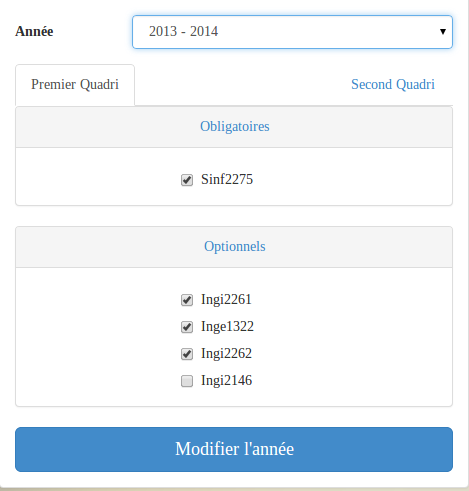
\includegraphics[width=\textwidth]{year_configuration}
\end{figure}

Lorsqu'un étudiant construit un programme, il configure essentiellement les cours de l'année qu'il va suivre et fait des prévisions sur les cours qu'il pourrait suivre l'année prochaine pour qu'il ne se trouve pas dans une situation où, en troisième année de bachelier par exemple, il ne puisse pas valider son programme.

Lorsque l'étudiant reprend son programme, l'année après sa validation par la commission, il doit recommencer ce processus. Il est cependant fort probable qu'une nouvelle version du programme de cours soit émise par la commission. C'est pourquoi il est possible via le bouton \textit{Mettre à niveau le programme} de mettre à jour celui-ci avec la nouvelle version disponible. Cette fonction va mettre à jour toutes les instances des cours constituant les années qui n'ont pas encore été créditées (ou partiellement créditées dans le cas d'une année ratée) avec celles de la nouvelle version du programme de cours (et toutes leurs contraintes par la même occasion). Les années (totalement ou partiellement) créditées sont automatiquement détectées par le module de contraintes. Celui-ci s'occupe d'aller chercher les contraintes correspondantes. 

Cependant, lorsque certains cours changent de sigle, il ne sera pas possible pour cette fonctionnalité de les récupérer. Si ce cours qui change de nom est le prérequis d'un autre cours, cette situation peut devenir problématique pour l'étudiant.  En effet, l'application ne sera pas capable de retrouver l'ancienne version du cours; l'étudiant aura donc une contrainte qu'il sera impossible de corriger.  Pour gérer cette situation, il est permis à l'étudiant de soumettre des programmes qui ne vérifient pas certaines contraintes, du moment qu'ils les justifient et que la commission de programme accepte cette justification. Il suffira à l'étudiant d'expliqué, dans le champ prévu à cet effet qu'il a déjà suivit l'ancienne version du cours.


\subsubsection{Vérification des contraintes}
Le module de gestion des contraintes renvoi beaucoup d'informations à propos des choses manquantes dans le programme. La page illustré sur la figure \ref{fig:constraint_mgmt} filtre ces informations et affiche essentiellement les dépendances manquantes.

\begin{figure}
\centering
\caption{Gestion des contraintes}
\label{fig:constraint_mgmt}
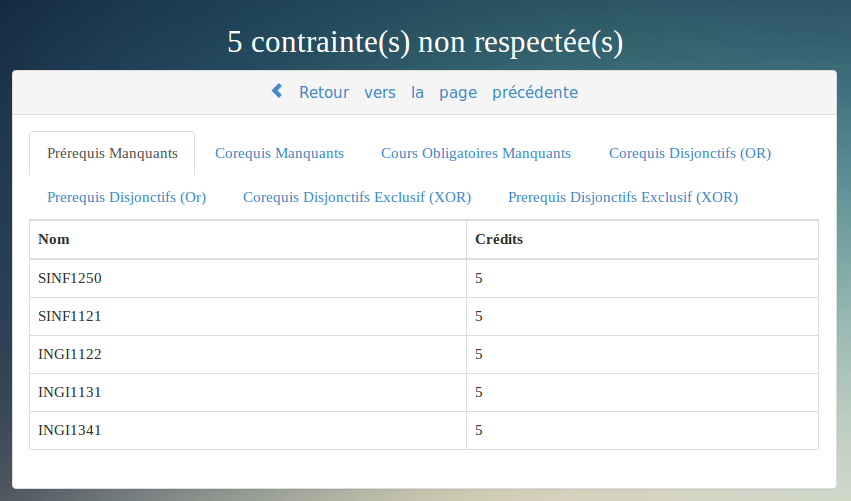
\includegraphics[width=\textwidth]{constraints_mgmt}
\end{figure}

\begin{figure}
\centering
\caption{Statut du programme d'un étudiant}
\label{fig:prgrm_status}
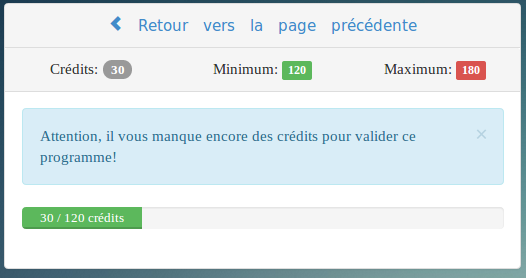
\includegraphics[width=\textwidth]{prgrm_status}
\end{figure} 

Toute les contraintes ne sont pas affichées sur cette page. La liste complète des contraintes gérées par le module qui gère les contraintes est la suivante:
\begin{itemize}
  \item les différentes dépendances entre les cours, telles qu'elles sont présentées sur la figure \ref{fig:constraint_mgmt};
  \item les contraintes relatives au nombre de crédits (crédits totaux, crédits minimum, crédits maximum) d'un ensemble de cours (programme ou module); en plus d'être affichées lorsqu'elles ne sont pas respectée, un menu récapitulatif (montrant la progression en terme de crédits du programme) est disponible en haut de la page \ref{fig:constraint_mgmt};
  \item les contraintes relatives au champ \textit{OBLIGATOIRE} d'un cours ou d'un module.
\end{itemize}

Comme expliqué dans la section \ref{prgrm_mgmt}, les contraintes temporelles sont gérées directement lorsqu'un cours est proposé à l'étudiant. En effet, une année se configure par semestre et, lorsque l'on configure le premier semestre par exemple, les cours du second semestre ne sont pas affichés. e 

C'est sur cette page \ref{fig:constraint_mgmt} que l'étudiant justifie \textbf{chacune des contraintes que son programme ne respecte pas}. Il n'est d'ailleurs pas possible d'envoyer le programme à la validation tant que chacune de ces exceptions n'a pas été justifiée.

\subsubsection{Négociation - Envoyer son programme à la validation}
 \label{validation_request}
Pour filtrer au maximum les demandes de validation et éviter ainsi de surcharger la commission de programme de requêtes inutiles, il n'est possible d'envoyer son programme à la validation que si certaines conditions sont respectées:
\begin{description}
  \item[avoir assez de crédits] le programme de l'étudiant doit respecter le minimum de crédits requis par le programme qu'il suit (dans le cas ou le programme ne propose pas suffisamment de cours, il suffit d'avoir autant de crédits que le programme en propose)
  \item[avoir accédé au menu de gestion des contraintes] à chaque fois que l'étudiant modifie son programme, il lui est demandé d'avoir visité au moins une fois la page relative à la vérification des contraintes pour pouvoir soumettre son programme;
  \item[ne pas avoir de dépendances non respectées ou avoir rempli le formulaire de justification] si le programme de l'étudiant comporte des contraintes non respectées, il lui est demandé de remplir un formulaire de justification dans lequel il doit justifier chacune des exceptions (contraintes non respectées);
  \item[ne pas avoir une requête en cours] si une requête a déjà été envoyée pour le programme, il n'est pas possible d'en envoyer une nouvelle tant que la précédente n'a pas été refusée ou acceptée par la commission de programme. Pour ne pas bloquer l'étudiant et demander à la commission de programme de faire plusieurs fois le travail de vérification, l'étudiant peut à tout moment annuler sa demande de validation, modifier son programme puis la renvoyer. 
\end{description} 

\subsection{Conclusion}
L'ensemble des fonctionnalités proposés aux deux types d'utilisateurs (étudiant et commission de programme) vient d'être présenté tout au long de cette section. Bien que cette section puisse servir de manuel, une version plus détaillée est présente en annexe expliquant plus en détail la démarche complète à suivre pour gérer les catalogues de cours et les programmes d'étudiant.

Notez que l'interface de l'application a été conçue pour être utilisée aussi bien sur un ordinateur que sur un smartphone. 

Cependant, il se peut que l'interface et certaines des fonctionnalités évoluent sensiblement suite au feedback récupéré après la remise des scénario de validation. 


% \subsection{Gestion des Données}
% \label{gestion_des_données}
% \subsubsection{Introduction}


% Il faut donc trouver un moyen de télécharger ces informations dans l'application. La solution la plus naïve serait de fournir des formulaires pour chaque entité (Cours, modules, ...) permettant d'ajouter une à une toute les informations nécessaire. Si l'on veut modifier les informations d'une entité, \textit{"il suffirait"} de naviguer dans les différents menu et de sélectionner le menu d'édition correspondant. Cependant cette solution n'atteint pas l'objectif fixé dans la solution, à savoir fournir un support pour enregistrer efficacement (et donc en peu de temps) les informations relatives aux curricula. Ajouter une à une toute les dépendances de cours peut être très ennuyant. 

% Une première amélioration que l'on peut ajouter à cette solution, est d'utiliser des formulaires excel pour ajouter ces informations. En créant une page par entité comme présenté sur l'image~\ref{fig:excel_example}, on pourrait ajouter toute les informations liés au modules, aux cours plus efficacement, l'import de fichier excel étant une chose assez aisée. 
% \begin{figure}[H]
% \centering
% \caption{Feuille Excel pour importer les données relatives aux modules}
% \label{fig:excel_example}
% 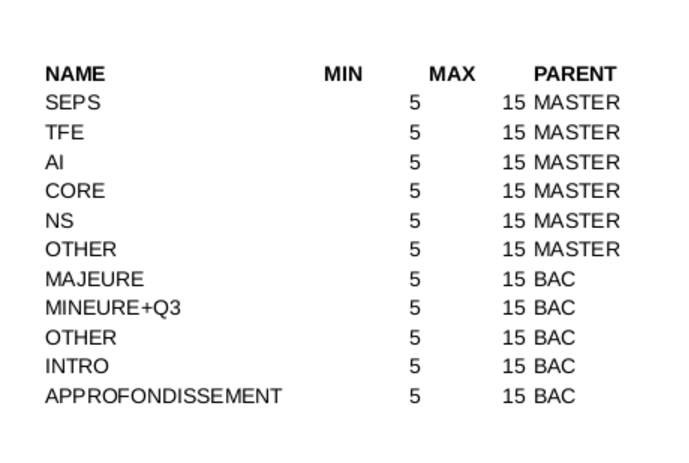
\includegraphics[width=0.8\textwidth]{excel_example}
% \end{figure} 

% Bien que cela permette d'ajouter des informations de façon plus efficaces, il subsiste plusieurs problèmes
% \begin{itemize}
% \item C'est toujours aussi éprouvant d'ajouter les dépendances. Il toujours les ajouter une par une, bien que cela soit sur une seule page.
% \item On ne peut pas donner au formulaire (et le programme qui l'importe) le pouvoir de créer les entités car:
% \begin{itemize}
%   \item En cas de faute de frappe, il faudra de nouveau naviguer dans l'application pour supprimer les erreurs.
%   \item Il est très difficile et peu efficace de gérer les inclusions des cours(L'appartenance d'une entité à une autre, un cours à un module par example). Cela implique des recherches sur le nom des entités. De nouveau, en cas de faute de frappe, il faudra aller corriger les erreurs dans l'application
% \end{itemize}
% \end{itemize}

% Le catalogue de cours étant un graphe (Dont les nœuds sont des entités et les dépendances des arrêtes), une autre solution serait d'utiliser un logiciel qui permet d'en dessiner. Un graphe étant visuellement plus parlant  qu'un tableur, le nombre d'erreurs serait donc moindre. 

% Le principal problème de cette solution réside dans les informations que l'on peut mettre dans ce graphe. Certes, on pourrait \textit{bricoler} avec le logiciel pour ajouter des méta-données aux objets que l'on dessine, mais cela pourrait de nouveaux devenir très embêtant à utiliser et surtout relativement compliqué à importer. 
  
% La solution utilisée dans l'application est un compromis entre la solution \textit{"graphe"} et celle \textit{"excel"}. La gestion des données est subdivisées en deux processus:
% \begin{itemize}
% \item L'import de la structure du catalogue via un logiciel qui permet de dessiner des graphes
% \item L'ajout d'informations supplémentaires (Nom, crédits, ...) via un import de formulaire excel
% \end{itemize}
% \subsubsection{Pourquoi avoir subdiviser l'import des données en deux parties distinctes?}

% Pour rendre les choses plus aisées au personnel qui va encoder le programme, nous avons décidé d'utiliser yEd, un outil relativement haut niveau qui permet de générer des graphes. En peu de temps, il est possible de construire l'ensemble du programme de cours à l'aide de cet éditeur disponible sur Windows, Mac Os et Linux tout en sortant un diagramme clair et concis.


% \textbf{Pourquoi}? Car le programme de cours est un graphe, dont chaque nœud correspond à un cours et chaque \textit{edge}, à une dépendance. 

% La solution idéale serait d'avoir un logiciel qui, en plus d'être intégré à l'application serait totalement adapté à notre besoin, à savoir \textbf{dessiner un graphe de cours}. Cela serait un dessinateur de programme de cours à part entière, proposant des nœuds intitulés cours, des arrêtes pour exprimer les contraintes, une façon de regrouper ces nœuds en module, en plus d'une autre pour y ajouter des informations relatives aux crédits, au contraintes des modules, etc. Cependant, cela dépasse malheureusement le cadre de mon mémoire. Libre à un étudiant, féru de développement web, de s'y attaquer dans les années à venir.

% \subsubsection{Limites de la démarche}
% Pour revenir à la façon dont nous importons les données, la principale limite d'un outil de la sorte est que nous sommes limités dans l'information que nous pouvons mettre dans ce graphe. Certes, il serait possible de sélectionner les différents nœuds et modules un à un et d'y ajouter l'information nécessaire, mais cette solution n'est pas efficace. Ils existe des solutions plus efficaces pour gérer des données à grande échelle : Excel.

% La seconde limite, est qu'il faut se mettre d'accord sur l'utilisation de ce programme tiers afin de savoir \textit{quoi} parser. Tout cela sera détaillé dans un manuel disponible dans les annexes

% L'import des données se fait donc en deux temps. Le graphe, qui contient les informations sur la structure du catalogue de cours (Nom des différentes entités et des dépendances), est d'abord parsé par l'application pour en extraire les informations. En suite, les informations plus spécifiques du catalogue de cours (les propriétés diverses des entités; nom détaillé, url, date, informations sur les crédits) doivent être fournies via un formulaire Excel qui, à sont, tour doit être télécharger vers l'application.

% \subsubsection{Construction et Import de la structure du catalogue}
% L'idée est de construire le graphe de cours en utilisant une application externe. Les exigences pour ce logiciel sont les suivantes:
% \begin{itemize}
% \item  Avec ce logiciel, il doit être possible de grouper les différents nœuds pour représenter les curricula et leur différents modules.
% \item Le graphe étant relativement complexe, il est nécessaire d'avoir un outil qui arrive à construire une disposition correcte
% \item Il doit être possible d'exporter ces informations dans un format standard et aisé à parser. 
% \item Ce logiciel doit être disponible sur Mac Os, Linux et Windows. 
% \end{itemize}

% Plusieurs candidats on été retenus; yEd, Dia et Graphiz. Tout les trois sont disponibles aussi bien sur Windows et Mac os que sur Linux et permettent d'exporter dans un format standard : le xml, mais un seul d'entre-eux permet de restructurer dynamiquement la structure du graphe: yEd.

% C'est pourquoi notre choix c'est porté sur ce logiciel.

% L'idée, pour construire le catalogue de cours, est (Dans yEd)
% \begin{itemize}
% \item D'utiliser les nœuds pour ajouter des cours, et de les labelliser avec leur sigle.
% \item D'utiliser les différents types d'arêtes pour représenter les différents types de dépendances
% \item De mettre les nœuds dans des groupes (labellisés avec leur nom) et les groupes dans des autres groupes pour représenter les différents modules, sous modules et programmes
% \end{itemize}

% Après, on demande au programme de calculer un layout hiérarchique. Sur l'image suivante, vous pouvez voir une partie de ce que génère yEd. (Le programme entier est disponibles dans les annexes)
% \begin{figure}[H]
% \centering
% 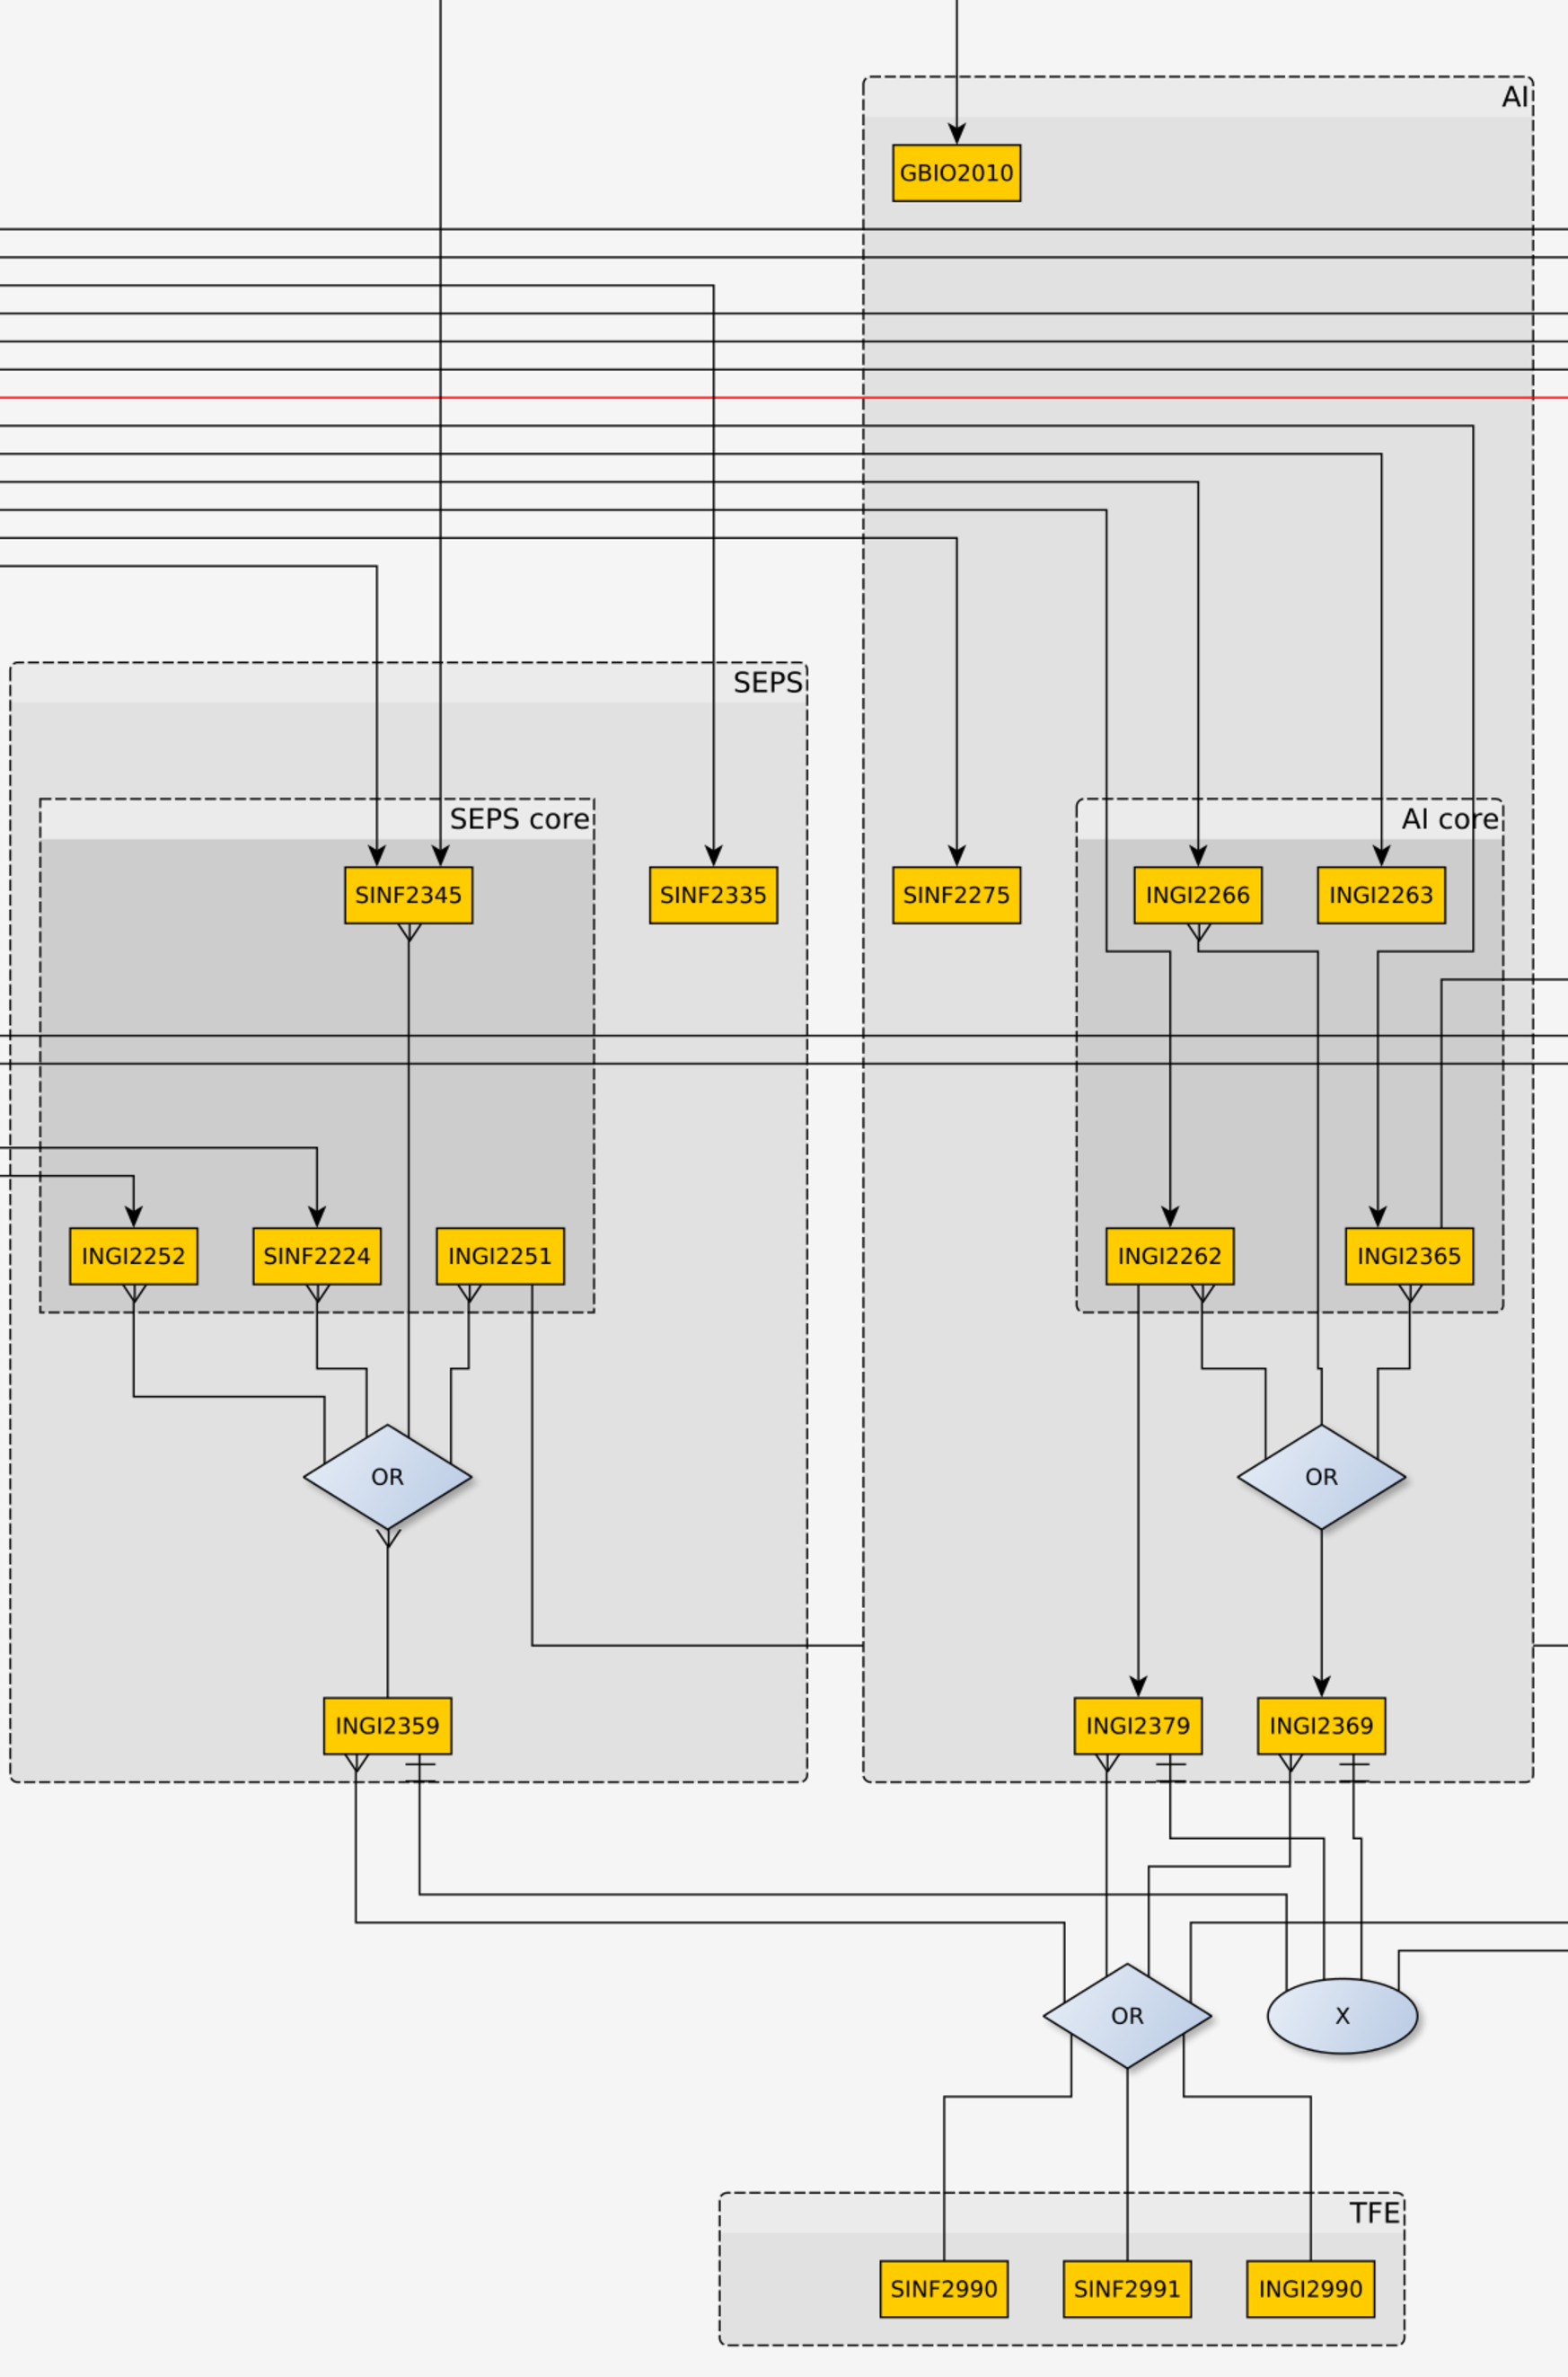
\includegraphics[width=\textwidth]{ingi_sub_course_catalog}
% \caption{Exemple de graph généré par Yed}
% \label{fig:subcatalog}
% \end{figure}


% \subsubsection{Construction et Import du formulaire Excel}
% Comme expliqué précédemment, le graph à lui seul n'est pas suffisant pour ajouter toute les informations nécessaire à l'application. Le formulaire Excel est utilisé pour ajouter les informations relatives au propriétés des programmes, modules et cours des différents curricula. 

% Ces propriétés contiennent des informations simples sur les différents objets du catalogues comme le nom complet des différents cours, modules et programmes, les professeurs, les liens vers pages des cours. Elle contiennent aussi les informations relatives aux contraintes sur les propriétés, comme le nombre de crédits.

% Il n'y a aucune restrictions sur les informations qui peuvent être ajoutées ici. 

% La structure du document est la suivante~\ref{fig:excel_structure}. Tout d'abord, il y a une page par objet (Cours, Programme, Module, Sous-module)

% \begin{figure}[H]
% \centering
% \caption{Structure d'un formulaire Excel}
% \label{fig:excel_structure}
% 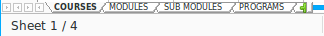
\includegraphics[width=0.8\textwidth]{excel_structure}
% \end{figure}

% Chacune des pages est structurée comme illustré sur l'image~\ref{fig:excel_page_structure}. 

% \begin{figure}[H]
% \centering
% \caption{Structure de la page relatives aux cours du formulaire Excel}
% \label{fig:excel_page_structure}
% 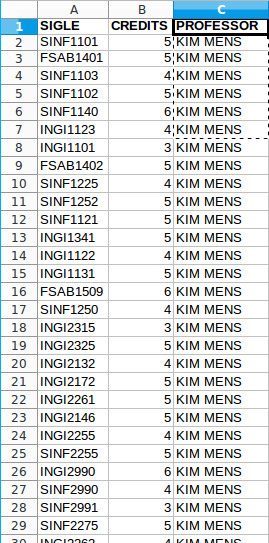
\includegraphics[scale=1]{excel_page_structure}
% \end{figure}

% La ligne 1, comprenant des cellules écrites en \textbf{gras} représente le header de la page. Chacune des cellules représente le nom de la propriété en question. Une propriété est un couple (Type, Value) où \textit{Type} correspond au nom de la propriété, et \textit{Value} à sa valeur. La première colomne représente la propriété qui \textbf{identifie} l'objet en question. Lorsque la page sera importé, une nouvelle propriété sera créée pour l'objet identifié par l'élément de la première colonne. La valeur de cette propriété sera la cellule traitée, et le type de la propriété le nom de la colonne. 

% Par exemple, pour la ligne 4 de la page~\ref{fig:excel_page_structure}
% Deux propriétés seront crées pour le cours intitulé \textit{SINF1103}
% \begin{enumerate}
% \item La propriété ayant pour type \textbf{CREDITS} avec comme valeur \textbf{5}.
% \item La propriété ayant pour type \textbf{PROFESSOR} avec comme valeur \textbf{KIM MENS}.
% \end{enumerate}

% Pour plus de facilité, il est possible de télécharger un \textit{template} de se formulaire depuis l'application, contenant toute les informations qui existe dans la base de données. 

% Par example, si l'on décide de télécharger ce template juste après avoir importer le graphe de cours, on aura les informations suivantes~\ref{fig:init_excel} pour les cours. 

% \begin{figure}[H]
% \caption{Formulaire excel téléchargé juste après importation du graphe}
% \label{fig:init_excel}
% 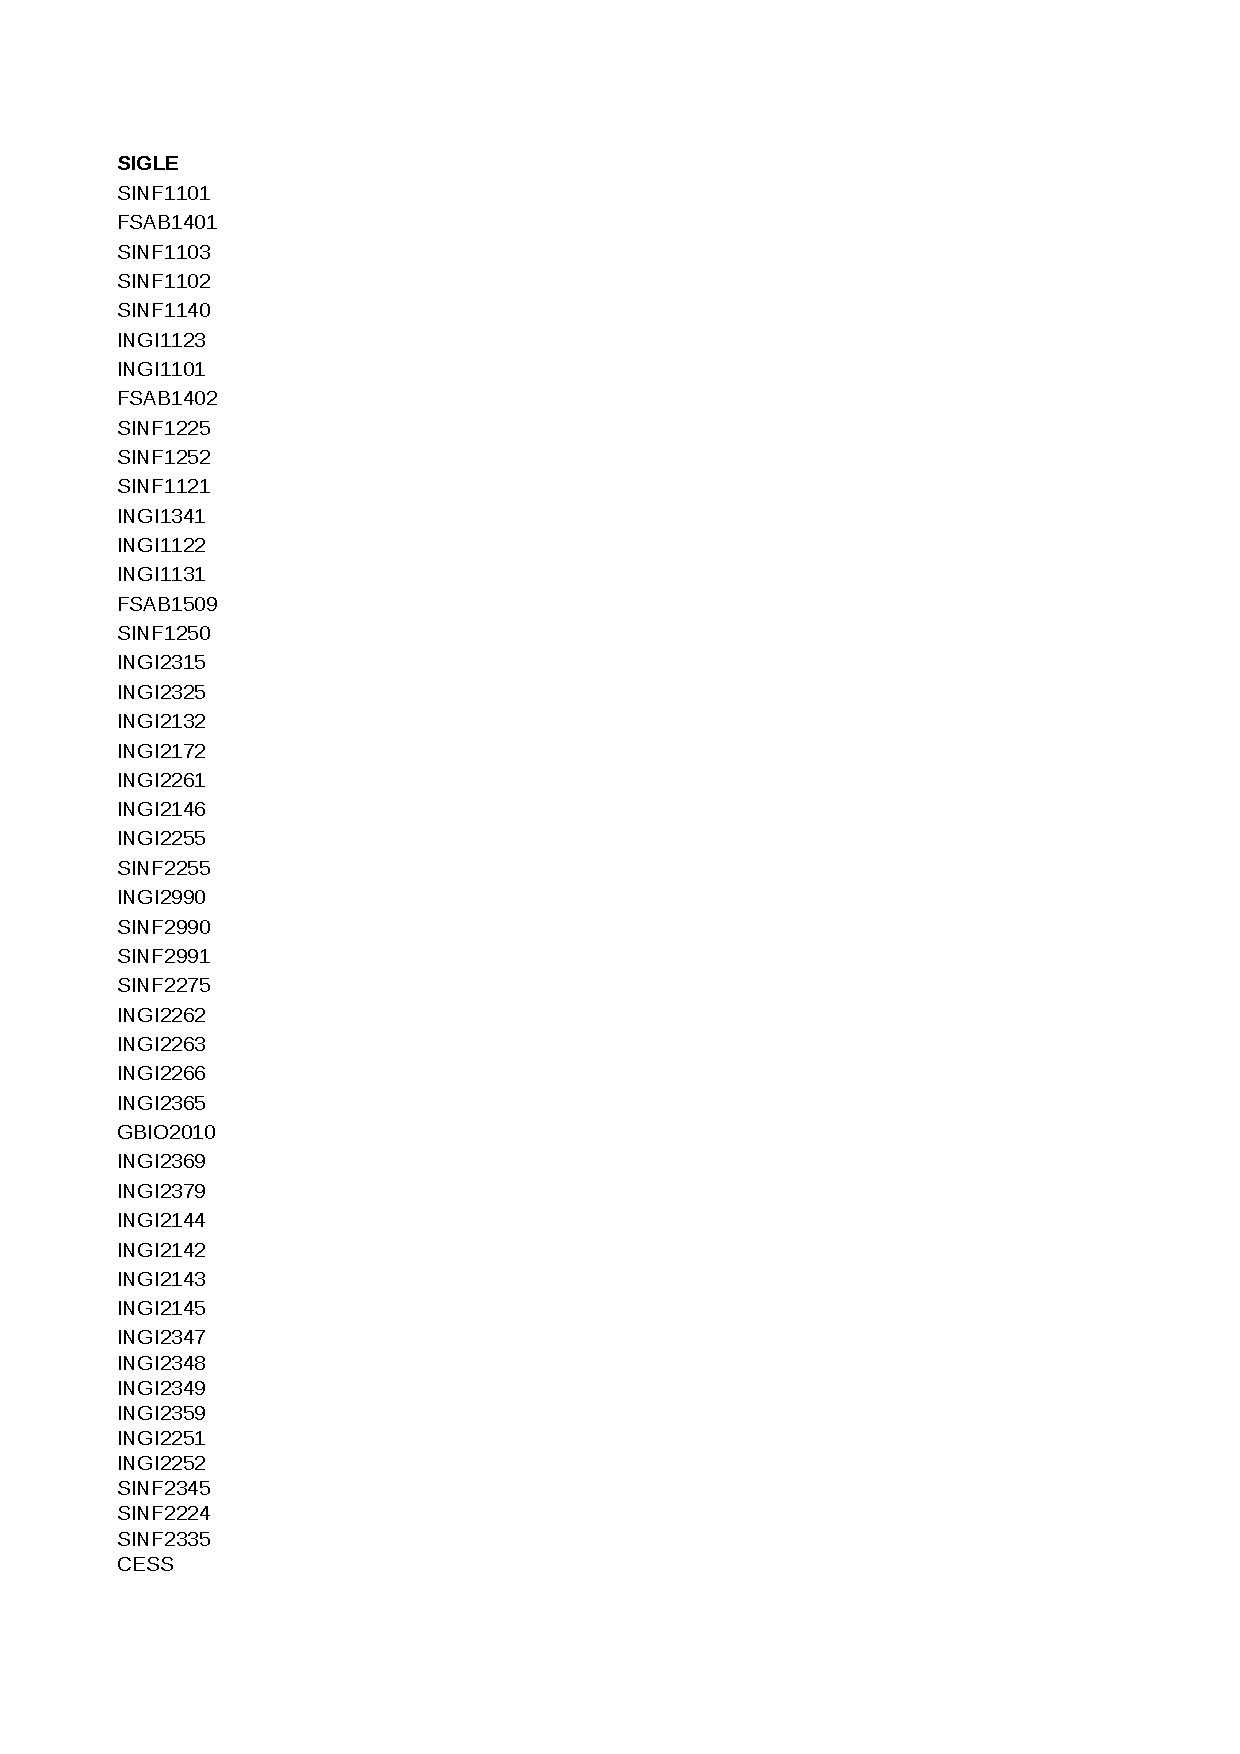
\includegraphics[scale=0.8]{init_excel}
% \end{figure}

% Il suffira après à la commission de programme de compléter ce fichier avec les informations souhaitées et de le télécharger vers l'application.

%         
\chapter{Développement du système}
\section{Introduction}
Le but poursuivit par ce chapitre est d'expliquer les choix qui ont influencé le développement de l'application et de chacun de ses modules externes, à savoir:

\begin{description}
  \item[ConstraintsChecker] le module qui s'occupe de vérifier la validité des programmes des étudiants;
  \item[XlsParser] le module qui s'occupe d'exporter les données des programmes de cours vers les formulaires et d'extraire les formulaires en provenance de la commission de programme;
  \item[GraphParser] le module qui s'occupe d'extraire les données en provenances des graphes que la commission de programme importe dans l'application.
\end{description}(ConstraintChecker, XlsParser et GraphParser). La structure du chapitre sera la suivante. 

La première section présentera l'architecture de l'application et de ses différents modules. On évitera ici de parler de l'architecture MVC car très peut de choix on été fait à ce niveau  (peu de libertés sont laissées par le framework au final). L'application gère et échange (avec ses modules) une grande quantité de données. Leur modélisation a un impacte critique sur les fonctionnalités de l'application (et leur implémentation). C'est pourquoi, l'accent sera mis ici sur la modélisation des classes de l'application.   

La deuxième section présentera les choix faits au niveau de l'implémentation des différentes fonctionnalités. Il sera expliqué par la même occasion comment ces fonctionnalités on été implémentées. 


\label{developpement_system}
\lhead{Chapitre 4 - Développement du système}
\section{Architecture}

\subsection{Architecture globale}

\begin{figure}
\caption{Architecture globale}
\centering
\label{fig:complete_arch}
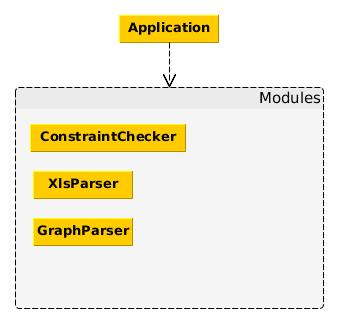
\includegraphics[width=\textwidth]{complete_arch}
\end{figure}

Ce modèle représente l'architecture de l'application et de l'ensemble de ses modules. L'objet application représente la partie \textit{Rails} de l'application. Cette partie comporte essentiellement les différents modèles, leurs vues et leurs contrôleurs (en plus de la base de données). L'application utilise trois modules développés indépendamment.
\begin{enumerate}
  \item \textbf{GraphParser} - le module s'occupant d'extraire l'information contenue dans les fichiers \textit{Graphml} générés par yEd, 
  \item \textbf{ConstraintCheker} - le module s'occupant de vérifier les contraintes des programmes d'étudiants
  \item \textbf{XlsParser} - le module occupant d'exporter les données relatives au programmes de cours vers un formulaire excel et d'extraire les informations contenues dans les formulaires excels que la commission importe via l'application. 
\end{enumerate}

Les informations manipulées par ces trois modules sont présentées en détail dans la section relative à la gestion des données du chapitre précédent \ref{data_mgmt}.

L'architecture de chacun de ces modules, en plus de celle de l'application sera expliqué dans les sous-sections qui suivent. Notez que la notation UML sera utilisée pour présenter les différents diagrammes de classe. 

Les conventions utilisées pour réaliser chacun des modèles sont les suivantes:


\begin{figure}[H]
\centering
\caption{Généralisation}
\label{fig:generalization}
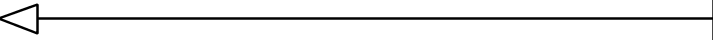
\includegraphics[width=\textwidth]{generalization}
\end{figure}

\begin{figure}[H]
\centering
\caption{Dépendance}
\label{fig:dependancy}
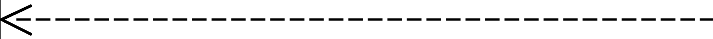
\includegraphics[width=\textwidth]{dependancy}
\end{figure}


\begin{figure}[H]
\centering
\caption{Association avec ses cardinalités}
 \label{fig:association}
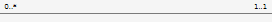
\includegraphics[width=\textwidth]{association}
\end{figure}

\begin{figure}[H]
\centering
\caption{Représentation d'une classe. En haut; les attributs, en bas; les méthodes.}
\label{fig:class_example}
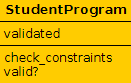
\includegraphics[scale=1]{class_example}
\end{figure}


\clearpage
\subsection{Application Rails}
\label{rails_arch}

Il y a plusieurs types d'associations en ruby on rails:
\begin{description}
  \item[Has One] - les cardinalité de cette association sont (0..1, 1..1); lorsqu'un objet A a une association \textit{has\_one} avec un objet B, B contient une référence vers l'objet A; 
  \item[Has Many] - les cardinalité de cette association sont (0..*, 1..*); lorsqu'un objet A a une association \textit{has\_many} avec un objet B, B contient une référence vers l'objet A;
  \item[Has And Belongs To Many] - les cardinalité de cette association sont (0..*, 0..*). Lorsqu'un objet a unne association \textit{has\_and\_belongs\_to\_many}, aucune référence n'est stockée dans les objets; à la place, une table intermédiaire est créée contenant l'id des deux objets.  
\end{description}

\label{arch}
\begin{figure}
\centering
\caption{Architecture de l'application}
\label{fig:app_arch}
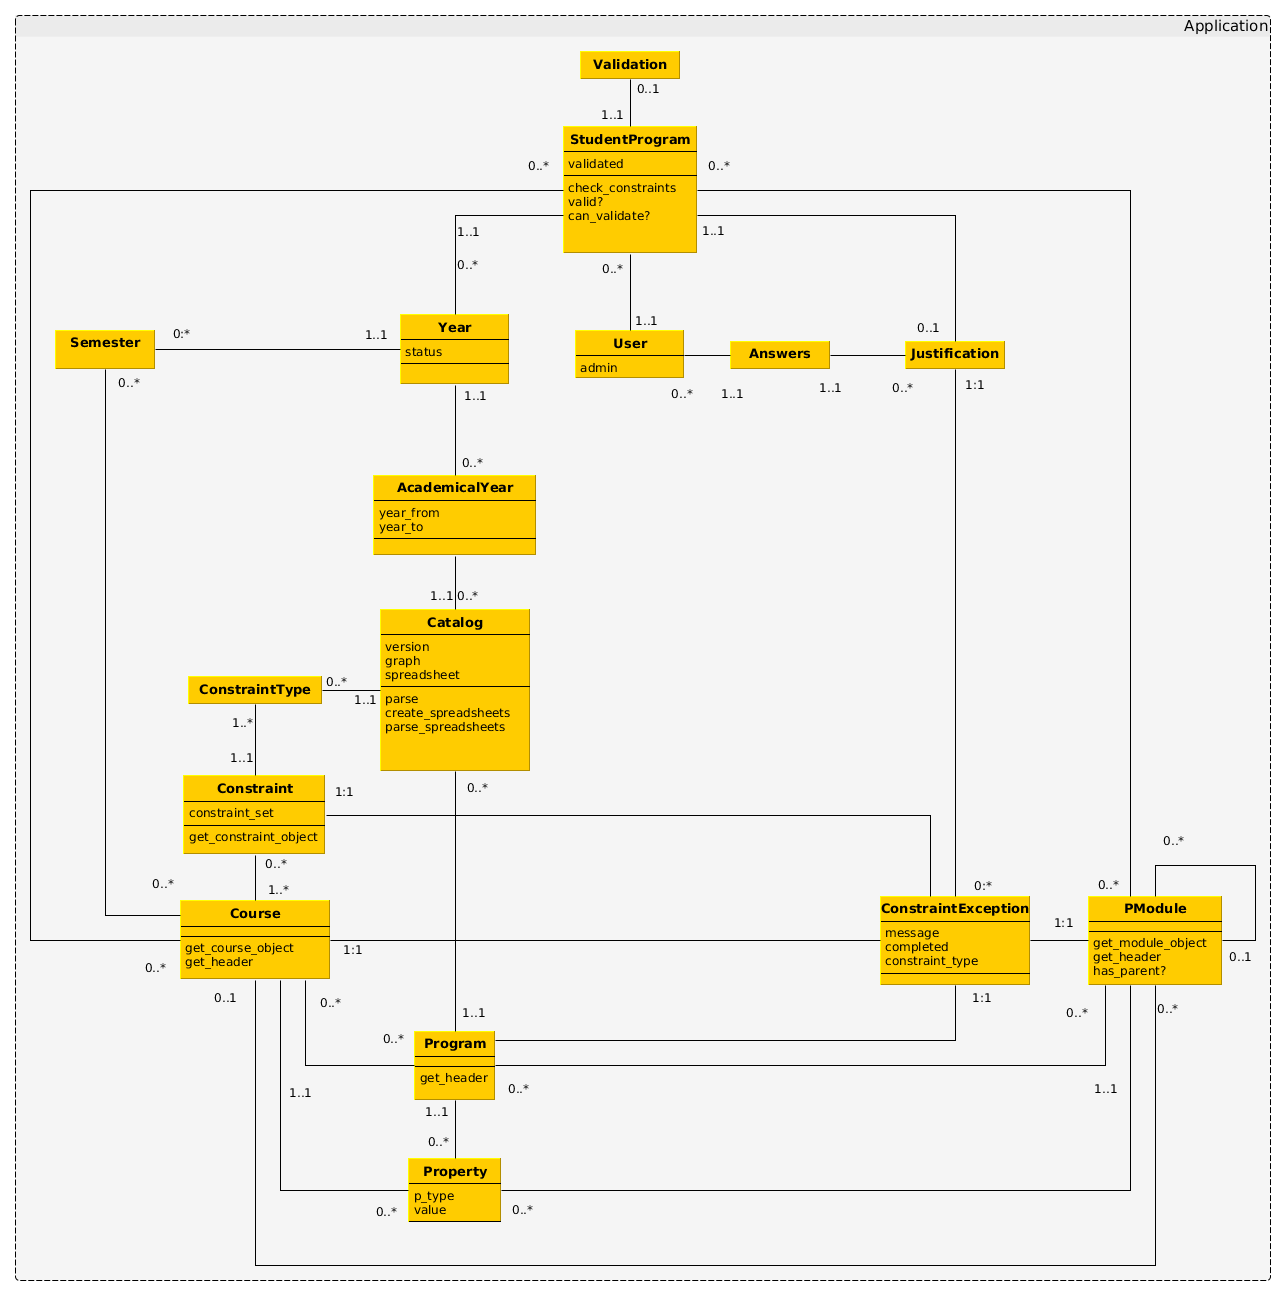
\includegraphics[width=\textwidth]{app_arch}
\end{figure}

\subsubsection{User} 

Cette classe représente les utilisateurs.  L'attribut \textbf{admin} sert à différencier les deux acteurs de l'application, à savoir la \textit{Commission de programme} et les étudiants. La section \ref{user_mgmt}
 explique en détail comment sont gérés les accès de ces deux types d'utilisateurs.

\subsubsection{Property}

Un objet \textit{Property} est composé d'un type et d'une valeur. Chacun des objets \textit{Program}, \textit{PModule} et \textit{Course} peu en avoir zéro ou plusieurs. Par exemple, pour représenter le sigle d'un cours, une propriété de type \textit{SIGLE} et de valeur \textit{SINF1101} sera ajoutée au cours correspondant. Il a été choisi d'opter pour cette solution, plutôt que d'ajouter des champs arbitraire (Sigle, crédits, ...) à chacun des objets car on ne sait pas à l'avance quelles seront leur propriété. En effet, elle sont déterminées par les informations mises dans le fichier excel qui est importé régulièrement dans l'application. 

\subsubsection{PModule}

C'est un ensemble de cours. Un \textit{PModule} peut avoir plusieurs \textit{PModule}. Ce comportement est justifié par le fait qu'un module de cours peut comporté un sous module qui comporte une série de cours obligatoires (L'option réseau et l'ensemble de ses cours obligatoires par exemple).

\subsubsection{Program}

Il représente un programme de cours. (Le programme de master par exemple) C'est un ensemble de cours et de modules divers. On peut créer des programmes via l'outil de graphes yEd, mais il est possible dans l'application de créer des Programmes \textit{à la carte} en choisissant les modules et cours qui le compose. C'est pourquoi il y a une relation \textit{many to many} entre \textit{PModule} et \textit{Program} et une autre entre \textit{Program} et \textit{Course}. En effet, chaque Programme peut avoir un ou plusieurs cours, et chaque cours peut appartenir à un ou plusieurs programmes (Le même comportement est observé pour les modules). Il n'est donc pas possible de représenter cette relation avec une relation \textit{has many} classique, qui implique d'avoir une références vers l'un des deux objets dans contenue l'autre. \cite{active_record}. 

\subsubsection{Catalog} 

Un catalogue est composé de plusieurs \textit{Program}, \textit{PModule} et \textit{Course}. Il contient aussi les informations à propos du fichier de graphe et du formulaire excel (nom, date, type). 

L'attribut \textit{version} est un entier qui représente la version du catalogue de cours. Il peut prendre trois valeurs différentes:

\begin{description}
  \item[0] version \textit{future};
  \item[1] version \textit{principale};
  \item[2] version \textit{ancienne}.
\end{description}

Les trois méthodes principales de cette classes sont:

\begin{description}
  \item[parse] qui appelle le module \textit{GraphParser}
  \item[parse\_spreadsheet] qui extrait les informations du formulaire excel (et upload la nouvelle version du formulaire sur le cloud).
  \item[create\_spreadsheet] qui crée le formulaire excel (et l'upload sur le cloud).
\end{description}

Les détails d'implémentation de ces méthodes seront expliquées dans la section relative au module avec lequel elles interagissent. 

\subsubsection{StudentProgram}

C'est le programme que se crée l'étudiant lorsqu'il utilise l'application. Un \textit{StudentProgram} est une instanciation d'un des \textit{Program} disponible dans le \textit{Catalog} utilisé (d'où la relation \textit{many to many}). De plus, un étudiant doit choisir les modules qu'il va suivre. Ce comportement est expliqué par la relation \textit{many to many} entre les deux modèles. Pour configurer son programme année par année, l'étudiant va se créer une année (\textit{Year})

La méthode \textit{can\_validate?} vérifie que certaines conditions sont remplies pour pouvoir envoyer un programme d'étudiant à la validation (Se référer à la section \ref{validation_request} pour plus de détail sur cette fonctionnalité).

La méthode \textit{check\_constraint} gère l’interaction avec le module \textit{ConstraintsChecker}. 

\subsubsection{Year}

Une année est composé de deux semestres. Un semestre est représenté par l'objet \textit{Semester}. L'attribut \textit{status} représente le fait qu'un programme d'étudiant aie été validé ou non par la commission. Le choix de chacun des cours du semestre est représenté par une association \textit{has\_and\_belongs\_to\_many} qui existe entre les deux objets.

Pour représenter le premier et le second semestre, un modèle \textit{FirstSemester} et un modèle \textit{SecondSemester} ont été créés, tout deux étendant le modèle \textit{Semester} en utilisant la \textit{Single Table Inheritance} de \textit{Rails} \cite{STI}. Notez que la relation entre ces deux types de \textit{Semester} et leur \textit{StudentProgram} est une \textit{has one} (la cardinalité est donc (1, 1) ici)

La choix d'utiliser la \textit{single table inheritance} est justifié par plusieurs raisons:
\begin{itemize}
  \item un objet \textit{year} étant composé de deux semestres, c'est plus clair d'utiliser deux associations \textit{has\_one} que d'utiliser une association \textit{has\_many} et de restreindre leur nombre par année en utilisant une validation; \textit{hardcodée}
  \item l'implémentation des formulaire de création d'année est plus aisée; on sait explicitement quel objet va représenter quel semestre;
  \item on laisse à rails le travail de devoir gérer le type de l'objet \textit{Semester} et comment devoir accéder à chacun de ceux-ci. Si l'on décide de changer le nombre de semestres par année, il suffit de créer un nouveau modèle qui étend \textit{Semester} et de rajouter la relation. Avec une solution conventionnelle, on devrait écrire du code pour représenter, créer et récupérer ce nouvel objet \textit{Semester} dans l'objet \textit{Year}. 
\end{itemize}


\subsubsection{Header}

Chacun des modèles \textit{Course}, \textit{Pmodule} et \textit{Program} contient une méthode get\_header qui renvoie une suggestion de propriétés utilisées à titre indicatif avec le module \textit{XlsParser} (voir \ref{xls_parser}) pour créer les formulaires excel. Nous avons le header suivant : \{"SIGLE", "CREDITS", "SEMESTRE", "OBLIGATOIRE"\} pour le modèle \textit{Course} par exemple.

\subsubsection{Méthodes get\_objet}
Ces méthode s'occupe de traduire les données concernant les contraintes des différents cours et modules en objet ruby. Ces objets sont par après manipulés par le module \textit{ConstraintsChecker}. 
\subsubsection{Constraints}
Cette classe représente les dépendances entre les cours. Le type de la dépendance est représenté par l'objet \textit{ConstraintType}. L'attribut \textit{set\_type} quant à lui représente le type de l'ensemble de contraintes. Comme expliqué dans la section \ref{contraintes}, une dépendance peut être une relation binaire entre un cours et sa dépendance. Elle peut être aussi une relation n-aire entre plusieurs cours et leurs dépendances.

Il existe deux association (bien qu'elles ne soient représentées que par une seule, par soucis de clarté, sur le diagramme de classes \ref{fig:app_arch}) qui relient les objets \textit{constraints} aux objets \textit{courses}. La classe \textit{Constraint} ne représentent que les contraintes de type dépendance, comme expliqué dans la section \ref{contraintes}. Ce type de contrainte ayant un cours source et un cours destination, il donc est nécessaire d'avoir deux relations.  La relation entre la destination et la contrainte est représentée par une association \textit{has\_many} entre le cours et la contrainte. La relation entre la source et la contrainte, quant à elle, est représentée par une association \textit{has\_and\_belongs\_to\_many}. 

Ce comportement est justifié par le fait que l'on accède aux contraintes depuis le cours \textit{destination}. C'est à dire que l'on va chercher les dépendances d'un cours, et non chercher la relation inverse, à savoir quels sont les cours pour lequel un cours joue le rôle de dépendance.

\subsubsection{AcademicYear}
Cette classe représente une année académique, c'est à dire composé de deux années. Elle est utilisée dans deux situations:
\begin{enumerate}
  \item identifier les objets \textit{Year} et \textit{Catalogue};
  \item gérer, du coté du module \textit{ConstraintsChecker} les dépendances de cours (on peut ainsi savoir quand à été suivit un cours). 
\end{enumerate}

\subsection{Architecture du vérificateur de contraintes}
\label{constraint_checker}
\begin{figure}[H]
\centering
\caption{Vérificateur de contraintes}
\label{fig:constraint_checker_arch}
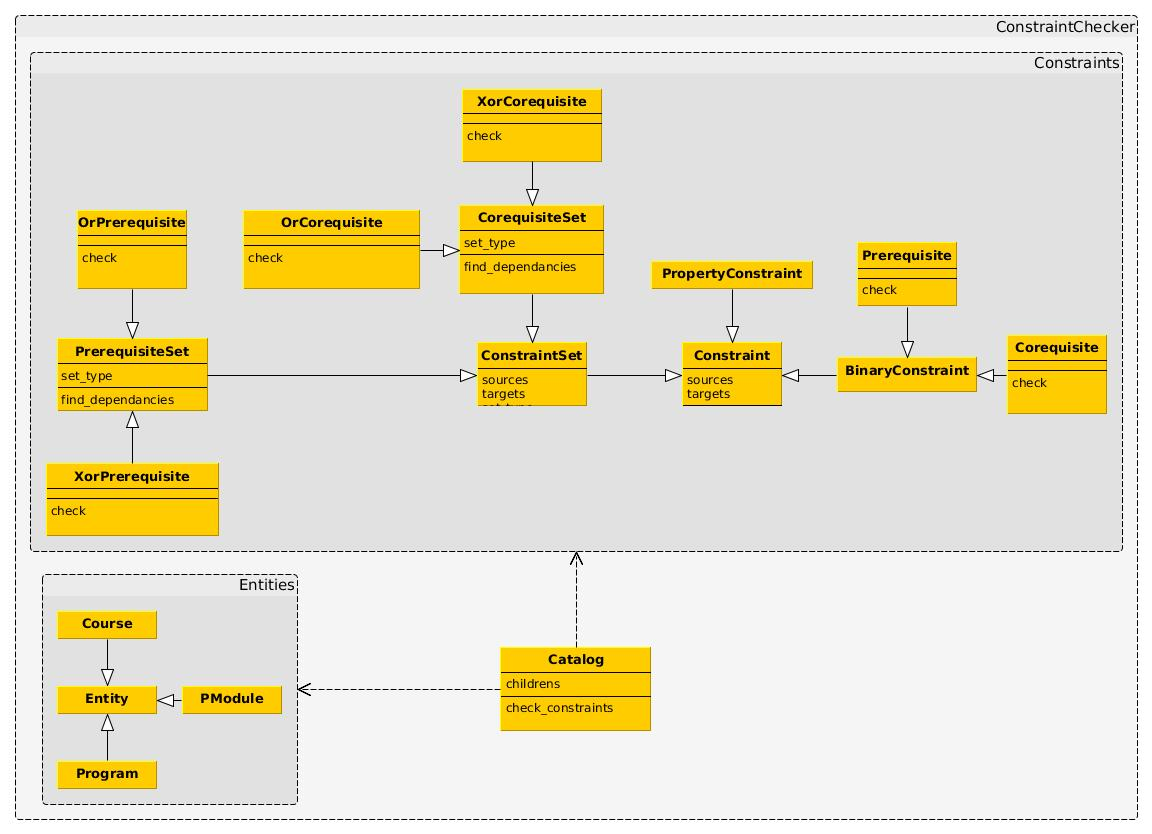
\includegraphics[width=\textwidth]{constraint_checker_arch}
\end{figure}

L'architecture de ce module est composé en deux parties;
\begin{enumerate}
  \item Les différents types de contraintes (Contraintes binaires, ensemble de contraintes ...)
  \item Les différents types d'entités (Cours, modules, ...)
\end{enumerate}

Le lien avec l'application se situe au niveau de la classe \textit{Catalog}. En effet, chacune des différentes entrées des tables concernées (courses, p\_modules, constraints) sont traduites en un objet entité.

L'idée ici est d'utiliser au plus l'héritage pour éviter d'avoir des duplications de code dans les classes. Par exemple, un objet \textit{Course} peut avoir beaucoup de contraintes mais chacune d’entre elles peut être de n'importe quel type. Cet objet n'a pas besoin de savoir le type de ses contraintes. Tout ce qu'il sait, c'est qu'il doit appeler leur méthode \textit{check} pour tester si les contraintes sont vérifiées. 


\subsection{Parser de graphes}

\begin{figure}[H]
\centering
\caption{Architecture du parser de graphe}
\label{fig:graph_parser_arch}
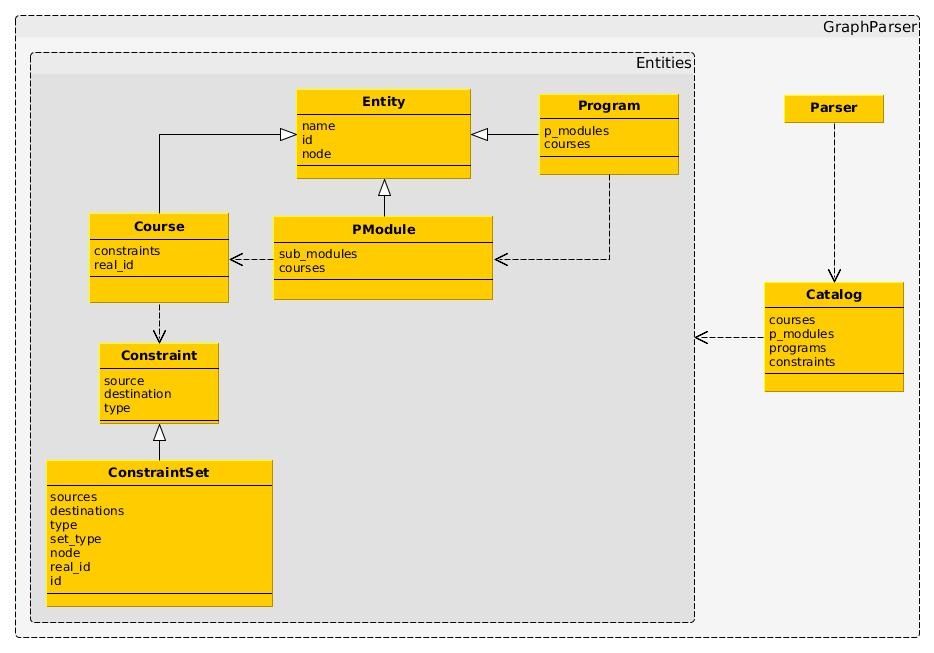
\includegraphics[width=\textwidth]{graph_parser_arch}
\end{figure}

Tout comme dans le vérificateur de contraintes \ref{constraint_checker}, le parser travail avec des objets \textit{entités} à la différence que c'est lui qui les fournit à l'application (et pas l'inverse)

De nouveau, l'héritage tient une page prépondérante ici, pour diminuer le couplage, augmenter la cohésion  et éviter autant que possible la duplication de code \cite{cohesion_couplage}. 

\subsection{Parser de fichiers excel}
\label{xls_parser}
\begin{figure}[H]
\centering
\caption{Architecture du parser de fichiers excel}
\label{xls_parser_arch}
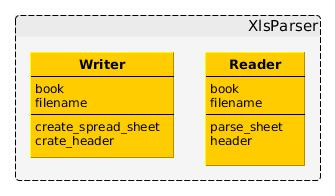
\includegraphics[scale=1]{xls_parser_arch}
\end{figure}

Ce module est relativement simple; il est composé de deux classe, un \textit{Writer} qui prend en input un tableau de donnée et un \textit{Reader} dont l'output est aussi un tableau de donnée.


\clearpage
%*************************************************************************************************************************************
\section{Implémentation}
\subsection{Hébergement de l'application}
L'application est hébergée sur \textit{Heroku}. Cela impose cependant quelques restrictions;
\begin{enumerate}
  \item On obligé d'utiliser postgresql comme système de base de données.
  \item Le répertoire de l'application est en lecture seule. On ne peut donc pas stocker le fichier de graphe et le formulaire excel dedans. Il est donc nécessaire d'utiliser un service de \textit{cloud storage} externe à l'application. Amazon S3 à été utilisé pour palier à ce problème. Pour rendre le téléchargement des fichiers vers ce service plus aisé, la gem \textit{Paperclip} a été utilisé. Les détails de configuration de ces différents services sont expliqués en annexes. 
\end{enumerate}
\subsection{Gestion des utilisateurs}
\label{user_mgmt}
Les utilisateur sont gérés à l'aide de deux gems. 

Devise est utilisé pour tout ce qui concerne la gestion des comptes (Création, modification, suppression), la gestion des sessions (Login/logout) et surtout la création de la table users et des différents attributs requis.

CanCan est utilité pour tout ce qui concerne les permissions des utilisateurs, à savoir à quel modèles un utilisateur à accès, et quels actions il peut effectuer sur ces modèles (Read, Create, Destroy, ...) 

Pour gérer les deux types d'utilisateur (Commission INFO et Étudiants, trois choix s'offrent à nous;
\begin{enumerate}
  \item générer avec devise deux tables séparées
  \item utiliser la Single Table Inheritance \cite{STI}. On crée un modèle user, puis on crée deux modèles spécifiques (student et admin) qui hérite de ce premier modèle
  \item générer un seul modèle user et y ajouter un attribut \textit{admin} pour identifier le rôle de l'utilisateur
\end{enumerate}

La troisième solution a été choisie. Elle permet d'éviter la redondance induite par la première solution et est plus simple à implémenter et à maintenir que la deuxième solution. En effet nos deux types d'utilisateur ne diffèrent que par leur rôle. 


La table générée par devise est la suivante;

\begin{lstlisting}
  create_table "users", force: true do |t|
    t.string   "email",                  default: "",    null: false
    t.string   "encrypted_password",     default: "",    null: false
    t.string   "reset_password_token"
    t.datetime "reset_password_sent_at"
    t.datetime "remember_created_at"
    t.integer  "sign_in_count",          default: 0,     null: false
    t.datetime "current_sign_in_at"
    t.datetime "last_sign_in_at"
    t.string   "current_sign_in_ip"
    t.string   "last_sign_in_ip"
    t.datetime "created_at"
    t.datetime "updated_at"
    t.boolean  "admin",                  default: false
  end
\end{lstlisting}

Pour vérifier si un utilisateur est connecté dans les vues, il suffit d'appeler le helper suivant

\begin{lstlisting}
user_signed_in?
\end{lstlisting}

Cela nous permet par exemple de cacher à l'utilisateur les menus permettant accéder aux différentes vues s'il n'est pas connecter

Pour vérifier si l'utilisateur à le rôle admin, il suffit de vérifier l'attribut dans la vue

\begin{lstlisting}
current_user.admin?
\end{lstlisting}

current\_user représentant l'utilisateur qui est connecté pour le moment.


Cependant, cela n'est pas suffisant. En effet, cela n'empêche pas l'utilisateur d'accéder aux différentes vues en entrant l'url dans la barre de navigation. C'est pourquoi il est nécessaire de dire à chaque contrôleur qu'il faut vérifier qu'un utilisateur est connecté avant d'afficher les vues. C'est fort heureusement très simple à faire avec Devise. Il suffit d'ajouter la ligne 
\begin{lstlisting}
before_action :authenticate_user!
\end{lstlisting}

dans chaque contrôleur où il est nécessaire que l'utilisateur soit connecté pour accéder aux vues. 

\textit{CanCan} intervient pour gérer les accès autorisés aux deux rôles de notre application (Utilisateur normal et admin). Il suffit simplement de créer un modèle \textit{Ability} dans lequel on décrit ce à quoi chaque rôle à accès. C'est de nouveau très simple;

\begin{lstlisting}
    if user.admin?
        can :manage, :all
    else
        can :manage, [StudentProgram, Year, Semester]
        can :create, Validation
    end
\end{lstlisting}

Il suffit de définir, en fonction du rôle de l'utilisateur, les modèles auxquels il a accès et ce qu'il peut faire. L'utilisateur \textit{normal} par exemple, n'a accès qu'aux modèles \textit{StudentProgram, Year, Semester}. S'il tente d'accéder aux vues des modèles auxquels il n'a pas accès, il sera redirigé vers la page d’accueil. 

Notez qu'il est possible de générer les vues qui permettent à l'utilisateur de s'enregistrer, de se connecter et de gérer les informations relatives à son compte utilisateur. Ces vues ont cependant été modifiées pour que leur style s'adapte à celui de l'application. 

Enfin, il n'est pas possible, pour des questions de sécurité évidentes, de se créer un compte \textit{admin} via les formulaires d'enregistrement disponibles dans l'application. Il faut tout d'abord se créer un compte utilisateur dans l'application, et ensuite modifier l'attribut \textit{admin} directement dans la console.  

\subsection{Importation du graphe}
\subsubsection{Introduction}
\label{graph_format_justification}
Une fois le graphe créé à l'aide de yEd, plusieurs choix s'offrent à nous pour exporter nos données. Les formats (non binaires) dans lesquels nous pouvons exporter les informations contenues dans notre graphe sont les suivantes. 
\begin{enumerate}
\item GraphML, un format de fichier basé sur XML pour les graphes
\item XGML, une alternative au format GraphML, mise en place par yWorks, la société qui développe le logiciel yEd
\item TGF (Trivial Graph Format) un format de fichier texte relativement simple pour décrire des graphiques
\end{enumerate}

TGF est de la forme

\begin{lstlisting}
1 SINF1101
2 FSAB1401
3 SINF1103
4 SINF1102
5 SINF1140
6 INGI1123
7 INGI1101
8 FSAB1402
9 NS //(Option network & security du programme Master)
\end{lstlisting}

et contient trop peu d'informations sur le graphe, comme les appartenances des cours aux différents modules et programmes. C'est pourquoi une solution basée sur XML a été choisie.

Voici ce à quoi ressemble les informations d'un fichier GraphML pour un noeud de type COURS.

\begin{lstlisting}
 <node id="n1::n3" yfiles.foldertype="group">
  <data key="d5"/>
    <data key="d6">
    (...)
  <node id="n1::n3::n2">
      <data key="d5"/>
      <data key="d6">
        <y:ShapeNode>
          <y:Geometry height="30.0" width="68.0" x="1136.0" y="1541.453125"/>
          <y:Fill color="#FFCC00" transparent="false"/>
          <y:BorderStyle color="#000000" type="line" width="1.0"/>
          <y:NodeLabel alignment="center" autoSizePolicy="content" fontFamily="Dialog" fontSize="12" fontStyle="plain" hasBackgroundColor="false" hasLineColor="false" height="17.96875" modelName="internal" modelPosition="c" textColor="#000000" visible="true" width="61.57421875" x="3.212890625" y="6.015625">SINF2335</y:NodeLabel>
          <y:Shape type="rectangle"/>
        </y:ShapeNode>
     </data>
  </node>
  (...)
</node>
\end{lstlisting}

En comparaison, la version \textit{XGML} du même nœud.
\begin{lstlisting}
<section name="node">
  <attribute key="id" type="int">69</attribute>
  <attribute key="label" type="String">SINF2335</attribute>
  <section name="graphics">
    <attribute key="x" type="double">1170.0</attribute>
    <attribute key="y" type="double">1556.453125</attribute>
    <attribute key="w" type="double">68.0</attribute>
    <attribute key="h" type="double">30.0</attribute>
    <attribute key="type" type="String">rectangle</attribute>
    <attribute key="fill" type="String">#FFCC00</attribute>
    <attribute key="outline" type="String">#000000</attribute>
  </section>
  <section name="LabelGraphics">
    <attribute key="text" type="String">SINF2335</attribute>
    <attribute key="fontSize" type="int">12</attribute>
    <attribute key="fontName" type="String">Dialog</attribute>
    <attribute key="anchor" type="String">c</attribute>
  </section>
  <attribute key="gid" type="int">61</attribute>
</section>
\end{lstlisting}

La principale différence entre le format XGML et GraphML se situe au niveau de la structure des informations. XGML structure toute les données de façon linéaire, en ne respectant pas la hiérarchie des différents nœuds et boites.

\begin{figure}
\centering
\caption{Exemple de graphe hiérarchique} 
\label{fig:hierarchical_graph_example}
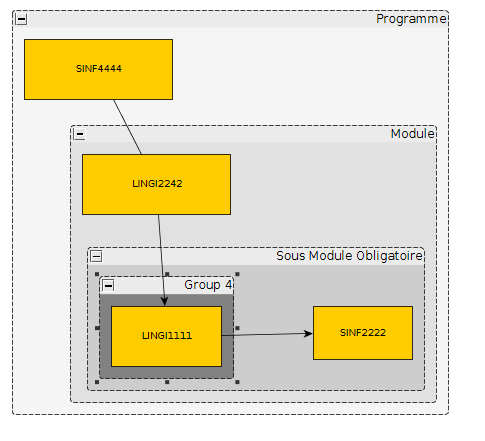
\includegraphics[width=\textwidth]{hierarchical_graph_example}
\end{figure}

Pour le graph \ref{fig:hierarchical_graph_example} par exemple, la structure d'un fichier XGML sera de la sorte:
\begin{lstlisting}
Node Programme
Node SINF4444
Node MODULE
Node LINGI2242
Node SOUS MODULE OBLIGATOIRE
(...)
\end{lstlisting}

Lorsque l'on parsera le fichier, on devra:
\begin{itemize}
  \item Parcourir le fichier, extraire les informations (nom, parent) de chaque cours, module et programme;
  \item Parcourir la liste des cours, modules et programmes pour ajouter les références vers leur parent et leurs enfants.
\end{itemize} 

Avec GraphML par contre, la structure  du fichier sera la suivante;

\begin{lstlisting}
Node Programme
Childs : [
  Node SINF4444
  Node MODULE
  Childs : [
    Node LINGI2242
    Node SOUS MODULE OBLIGATOIRE
    Childs : [
    ]
  ]
]
(...)
\end{lstlisting}

Lorsqu'on parsera le fichier; on devra simplement extraire les informations comme précédemment. On saura par contre au moment ou l'on parse un objet à quel parent il appartient.  Il n'est donc pas nécessaire de retraiter tout les éléments pour compléter les informations à propos de leur parent et de leurs enfants. Ceci est la principale raison pourquoi \textit{Graphml} est le format supporté par l'application.


\subsubsection{Parsing}
\label{graph_parsing}
Le but de ce module est de fournir une abstraction supplémentaire à la gem \textit{Nokogiri}\footnote{Librairie ruby permettant de parser des fichiers XML} pour extraire les informations contenues dans le fichier \textit{GraphML} de yEd. Les informations contenue dans le graphe généré avec \textit{yEd} sont les suivantes:
\begin{itemize}
\item Les Programmes de cours (Bachelier, Masters)
\item Les Modules et leur nom
\item Les Sous-modules et leur nom
\item Les cours et leur sigle
\item Les contraintes hiérarchiques (Qui contient quoi)
\item Les dépendances entre les cours (Corequis et Prérequis)
\end{itemize}

Ce module est appelé par le modèle \textit{Catalogue} de l'application à sa création. Le fichier graphe est d'abord envoyé sur le  \textit{cloud amazon}, puis parsé par le module \textit{GraphParser}. Une fois le parsing terminé, les différents objets (Cours, Modules et Programmes) sont récupérés par le modèle \textit{Catalogue}, puis traités par chacun des modèles concernés, avant d'être enregistrés en base de données. 

Tout ces éléments sont représentés par des nœuds dans le fichier GraphML. Seul les dépendances entre les cours sont représentées par des arrêtes dans le graphes, nommées \textit{Edge} dans le fichier. Les nœuds sont stockés en premier dans le fichier de graphe, suivit par toute les arrêtes. 

Le module ajoutes deux fonctionnalités à \textit{Nokogiri}.
\begin{enumerate}
  \item Il parse un fichier GraphML et extrait les métadonnées de ses nœuds (type, enfants, parent) et arrêtes (source, destination, type de contrainte, type de l'ensemble de contrainte). 
  \item Il renvoie des objets cours, modules et programmes ainsi que leur différentes dépendances.  
\end{enumerate}

 Comme expliqué dans l'introduction de cette section, chaque élément peut avoir un enfant, est identifié par un tag, peut avoir des attributs et contient de l'information. 

 la structure plus détaillée d'un nœud est la suivante:

\begin{lstlisting}
<node id="parentID::nodeID" [GROUP]>
  <(...)>
  </(...)
  <NodeLabel>
    NAME
  </(...)
  <(...)>
  </(...)>
</node>
<graph id="parentID">
  <node id (...)>
  <node id (...)>
</graph>
\end{lstlisting}

Il y a donc quatre informations à extraire;
\begin{enumerate}
  \item l'identifiant du nœud parent (parentID);
  \item l'identifiant du nœud (nodeID);
  \item son nom (NAME);
  \item est-ce un groupe? (GROUP)
\end{enumerate}

La structure de graphe imposée à la commission est la suivante; 

\begin{itemize}
\item les modules et programmes sont représentés par des nœuds \textit{Group};
\item les cours sont représentés par des simple nœuds;
\item les dépendances par des arrêtes.
\end{itemize}

Notez que chaque cour et module \textbf{DOIT} se trouver dans un programme. En effet, \textit{nœuds groupes} sans parents sont interprétés comme programmes. Cela nous permet de distinguer les modules des programmes, sans devoir ajouter une convention de couleur sur les boites pour les différencier.  

L'algorithme de parsing est donc relativement simple.

On a;
\begin{itemize}
  \item une méthode qui parse les arrêtes; 
  \item une méthode qui parse les nœuds;
  \item une méthode qui aprse les programmes et ses enfants;
  \item une méthode qui parse les modules et ses enfants;
  \item une méthode qui parse les cours.
\end{itemize}

On crée au préalable un \textbf{objet} catalogue. Chacune des méthodes listées précédemment renvoie un \textbf{objet} Cours, Module, Programme, Contrainte. Ces objets sont ajoutés au catalogue en respectant leur hiérarchie. Un cours aura donc comme parent un module ou un programme. 


\begin{lstlisting}
FOREACH element in graph do
- IF node -> 
  parse node
  - IF program -> 
    parse program (extract informations and add to catalog)
    (1) parse childs
      - IF module
        -> parse module (extract informations and add to parent)
        -> parse childs (go_to (1))
      - IF course
        -> parse course (extract informations and add to parent)


- IF edge -> 
  parse edge
    retrieve sources
    retrieve destinatinations
    retrieve constraint type
    FOREACH course in destinations do
      add new contraint to course
\end{lstlisting}


Une fois le parsing terminé, toutes les informations contenues dans chacun des \textbf{objets} cours, modules et programmes et contraintes sont ajoutés dans la table correspondante en base de donnée. 


\subsection{Gestion des contraintes}
Les contraintes sont vérifiées au niveau du modèle \textit{StudentProgram}, le modèle qui contient les informations à propos des programmes de cours des étudiants (C'est ce modèle qui appelle le module \textit{ConstraintsChecker}. 

Le module \textit{ConstraintsChecker} est divisé en deux parties. D'un coté nous avons les contraintes. Tout les types de contraintes héritent de la super classe \textit{Contrainte} qui, en plus de constructeur ne contient qu'une seule méthode \textbf{Check}. De l'autre coté nous avons les entités qui représentent les modèles \textit{Course}, \textit{Module} et \textit{Program}

\subsubsection{Entités}
\textit{Entity} est la classe qui représente les objets traités par le module \textit{ConstraintsChecker}. Entity étends la classe OpenStruct. Openstruct est une librairie qui permet de créer des objets à la volée. Pour chaque paramètre passé à un objet \textit{OpenStruct} \cite{OpenStruct}, un attribut sera créé ainsi que les méthodes pour le modifier et y accéder. On évite ainsi de devoir modifier la classe \textit{Entity} et ses enfants {Course, PModule} lorsque l'on veut rajouter une contrainte ou une nouvelle propriété par exemple.

Nos différents objets sont stockés sous forme d'arbre. La racine est l'objet catalogue, et les enfants sont les différents objets \textit{Course} et \textit{PModule}, tous étendant le super-type \textit{Entity}.

Un objet \textit{entity} contient essentiellement;

\begin{itemize}
  \item un attribut \textbf{constraints} qui contienne les différentes contraintes de l'objet;
  \item un attribut \textbf{childrens} qui contient les références vers ses enfant dans l'arbre;
  \item un attribut \textbf{parent} qui contient la référence vers son parent dans l'arbre;
  \item une méthode \textbf{find\_children(children\_id, children\_type)} qui permet d'effectuer une recherche sur ses enfants. Le paramètre \textit{children\_type} permets de spécifier le type d'enfant que nous recherchons (Cours, PModule);
  \item une méthode \textbf{search(children\_id, children\_type)} qui permet d'effectuer une recherche dans tout l'arbre. Cette méthode est utilisé dans les methodes \textit{check} des différentes contraintes pour retrouver des objets \textit{Course}. (Retrouver une dépendance par exemple). L'algorithme est le suivant;
  \begin{lstlisting}
  - Retrouver la racine de l'arbre
  - Appeler find_children sur ses enfants
  \end{lstlisting}
  \item une méthode \textbf{check} qui vérifie ses contraintes et celle de ses enfants;
  \item des méthodes relatives aux différentes contraintes, comme \textit{count\_credits}, \textit{check\_max}, \textit{check\_min}, \ldots
\end{itemize}

Ces objets sont construits dans les différents modèles de l'application. L'idée, dans chacun de ces modèles (Course, PModule, Constraint) est d'avoir une méthode get\_[model\_name]object qui va créer l'objet correspondant.

Dans le cas du modèle \textit{Course}, la méthode est la suivante:


\textbf{Course}

\begin{lstlisting}
def get_course_object(start_year, end_year)
  course = ConstraintsChecker::Entities::Course.new(name: self.name, id: self.id, start_year: start_year, end_year: end_year, parent_id: self.p_module_id, credits: self.credits, mandatory: self.mandatory?)
  self.constraints.each do |c|
    course.add_constraint(c.get_constraint_object(course))
  end
  return course
end
\end{lstlisting}


Les paramètre \textit{start\_year} et \textit{end\_year} identifient l'année académique au cours de laquelle un cours a été suivie dans un programme d'étudiant. Ces informations sont utilisés lors de la vérification des dépendances. 

Dans le cas d'un prérequis  par exemple, l'algorithme va vérifier que l'année académique durant laquelle a été suivie le cours est strictement antérieure à l'année académique du cours pour le quel il est un prérequis. Ce mécanisme gère aussi bien les années réussies que les années ratées. En effet, dans le cas d'une année raté, la commission aura au préalable sélectionner les cours qui on été réussis. Les cours ratés (qui ne sont pas sélectionnés) seront retiré de l'année en question. Il ne seront donc pas présent dans \textbf{objet} catalogue lors de la vérification des contraintes. 

Comme expliqué plus haut, on peut passer au constructeur de \textit{Course} tout ce que l'on veut, grâce à OpenStruct \cite{OpenStruct}.

Rien ne nous oblige à passer par le modèle \textit{Constraint} pour ajouter les contraintes. Comme expliqué dans la section \ref{rails_arch} (présentant l'architecture de l'application) , seul les dépendances sont représentés par l'objet \textit{Constraint} en base de données. En effet la plupart des données relatives à ces contraintes sont, en plus d'être présentes en base de données, assez volatiles, car elles peuvent être modifiées régulièrement via l'import de fichiers excels. Nous évitons ainsi de surcharger notre architecture avec des objets dont l'utilité est plus que relative. Pour revenir à ce type de contraintes, il est préférable de les ajouter dans la méthode \textit{get\_[model\_name]object} (la méthode du modèle qui crée l'objet \textit{Entity}.

\textbf{PModule}

\begin{lstlisting}
def get_p_module_object(mandatory)
  p_module = ConstraintsChecker::Entities::PModule.new(id: self.id, name: self.name)
  p_module.add_constraint(ConstraintsChecker::Constraints::Min.new(p_module, self.min))-
  p_module.add_constraint(ConstraintsChecker::Constraints::Max.new(p_module, self.max))
  self.sub_modules.each do |m|
    p_module.add_children(m.get_p_module_object(true))
  end

  if mandatory
    course_ids = []
    self.courses.each do |course|
      course_ids << course.id
    end
    p_module.add_constraint(ConstraintsChecker::Constraints::Mandatory.new(p_module, course_ids))
  end

  return p_module
end
\end{lstlisting}

Le paramètre \textit{mandatory} sert à identifier si le module est obligatoire ou non. Cela est utile pour vérifier si les cours d'un module obligatoire on bien été suivis.
Nous avons ici un exemple de contraintes (Min \& Max) qui ne sont pas ajoutées en passant par le modèle \textit{Constraint}. 


\subsubsection{Contraintes}
L'idée, pour chaque type de contraintes, est d'étendre la super-classe \textit{Constraint} en ré-implémentant la méthode \textit{check} pour qu'elle corresponde au comportement recherché. Cette méthode renvoie un \textit{hash}, spécifique à chaque type de contraintes, contenant les résultats de la vérification.

Par exemple, pour les dépendances entre les cours nous avons deux types. Les dépendances binaires, qui correspondent à un prérequis ou corequis entre deux cours, et les dépendances n-aire qui correspondent à un ensemble de prérequis ou corequis entre plusieurs cours avec une condition sur cet ensemble de contraintes. Cet ensemble peut être une disjonction (OR) de contraintes par exemple, exprimant qu'il faut choisir au moins une des dépendances, ou une disjonction exclusive (XOR), exprimant qu'il faut choisir une et une seule dépendance. 

Prenons l'exemple des dépendances binaires. Nous avons une classe \textit{BinaryConstraint} qui ne ré-implémente pas la méthode check de sa super-classe \textit{Constraint} car elle sert de super-classe pour les deux classes représentant les deux types de contraintes; \textit{Prerequisite} et \textit{Corequisite}. 

\begin{description}
  \item[Corequisite] La méthode check va appeler la méthode \textit{find\_course} du cours en question, qui va remonter jusqu'à la racine (le catalogue), et chercher si le corequis du cours est présent dans le catalogue.  S'il est présent, il va vérifier qu'il n'est pas suivit dans une année postérieure au cours pour le quel il est un corequis (conformément à la définition d'un prérequis \ref{contraintes}). Si la vérification précédente échoue, ou si le cours n'est tout simplement pas présent, le message ``corequisite\_missing :[course\_id]'' est envoyé.
  \item[Prerequisite] La méthode check se comporte comme celle de \textit{Corequisite}, à la différence que la vérification de l'année académique est plus stricte: le cours doit être suivit dans une année strictement antérieure (conformément à la définition d'un prérequis \ref{contraintes}). 
\end{description}

Dans le cas d'un ensemble n-aire de contraintes, il y a essentiellement deux points qui diffèrent;
\begin{enumerate}
  \item l'existence d'une méthode \textit{find\_dependancies} qui récupère les \textit{course\_id} manquants pour la contrainte en question en vérifiant aussi les années académiques;
  \item une vérification sur la taille de la liste, correspondant à la condition qui régit cet ensemble de contrainte. Dans le cas d'un ensemble disjonctif (OR), il faut vérifier que le nombre de \textit{course\_id} renvoyé soit strictement inférieure au nombre de dépendances du cours, pour vérifier qu'il y ai au moins une dépendance qui est choisie, conformément à la logique d'une disjonction. Dans le cas d'un ensemble disjonctif exclusif (XOR), il faut vérifier qu'il n'y aie qu'une et une seule dépendance choisie, conformément à la logique d'une disjonction exclusive.
\end{enumerate}

Pour vérifier ces contraintes, l'objet \textit{Catalog} appelle sur chacune des contraintes de ses enfants et de leur enfants leur méthode \textit{check} et récupère les messages qu'elles renvoient. Ces messages sont traités par le modèle \textit{StudentProgram} et affichés sur les vues correspondantes.

À ce jour, la liste des messages renvoyés par les méthodes \textit{check} des différents types de contraintes est la suivante:

\begin{description}
\item[or\_corequisites\_missing] Ce message concerne la contrainte n-aire \textit{OR-Corequisite}. Il contient la liste des ids des cours concernés par la contrainte si elle n'est pas vérifiée;
\item[xor\_corequisites\_missing] Ce message concerne la contrainte n-aire \textit{XOR-Corequisite}. Il contient la liste des ids des cours concernés par la contrainte si elle n'est pas vérifiée;
\item[or\_prerequisites\_missing] Ce message concerne la contrainte n-aire \textit{OR-Prerequisite}. Il contient la liste des ids des cours concernés par la contrainte si elle n'est pas vérifiée;
\item[xor\_prerequisites\_missing] Ce message concerne la contrainte n-aire \textit{XOR-Prerequisite}. Il contient la liste des ids des cours concernés par la contrainte si elle n'est pas vérifiée;
\item[prerequisites\_missing] Ce message concerne la contrainte binaire \textit{Prerequisite}. Il contient l'id du cours concerné par la contrainte si elle n'est pas vérifiée;
\item[corequisites\_missing] Ce message concerne la contrainte binaire \textit{Corequisite}. Il contient l'id du cours concerné par la contrainte si elle n'est pas vérifiée;
\item[to\_few\_credits] Ce message concerne la contrainte sur la propriété (Crédits) \textit{Min}. Il contient l'id de l'entité concerné par la contrainte si elle n'est pas vérifiée;
\item[to\_many\_credits] Ce message concerne la contrainte sur la propriété (Crédits) \textit{Max}. Il contient l'id de l'entité concerné par la contrainte si elle n'est pas vérifiée;
\item[courses\_missing\_in\_module] Ce message concerne la contrainte sur la propriété \textit{Mandatory} d'un objet \textit{Module}. Il contient les ids des entités manquantes d'un Module; obligatoire si la contrainte n'est pas vérifiée;  
\item[mandatory\_courses\_missing] Ce message concerne la contrainte sur la propriété \textit{Mandatory} d'un objet \textit{Course}. Il contient l'id du cours en question si la contrainte n'est pas vérifiée.
\end{description}

Pour ajouter un nouveau type de contraintes, il faut procéder comme suit;

\begin{enumerate}
  \item Si le type de la contrainte ne rentre pas dans la catégorisation des contraintes déjà existantes (BinaryConstraint, PropertyConstraint, NaryConstraint), il faut créer une nouvelle classe. Sinon, il suffit d'étendre la classe existante.
  \item Implémenter la méthode \textit{check} de cette contrainte avec le comportement désiré. Il ne faut pas oublier de renvoyer à la fin de cette méthode un message qui \textit{explique} pourquoi la contrainte n'est pas vérifiée, en cas d'échec
  \item Dans la méthode \textit{get\_object} du modèle concerné par la contrainte, créer et ajouter l'objet contrainte et ajouter les informations nécessaire dans l'objet créé par le modèle. Par exemple, si je rajoute une contrainte sur les crédits, il faut passer le paramètre \textit{credits: value} au constructeur de l'objet \textit{Entity::Course}
\end{enumerate}



\subsection{Importation du formulaire Excel}
Le module est composé de deux parties: 
\begin{enumerate}
\item Un \textit{Reader} qui propose une fonction pour récupérer sous forme de tableau de \textit{Hash} les informations d'une page Excel, en lui fournissant \textbf{le nom de la page}, ainsi que \textbf{la propriété qui est utilisée pour identifier l'objet} (Le sigle pour les cours par exemple).
\item Un \textit{Writter} qui propose une fonction pour écrire des données dans une page d'un document Excel.
\end{enumerate}

L'intérêt de fournir une abstraction supplémentaire se situe sur la structure des documents échangés avec l'utilisateur. En effet, chaque document comporte plusieurs pages. Chacune d'entre elles contient des informations sur un des objets (Course, Sub-Module, Modules ou Program). Ces informations sont représentées par le Modèle \textit{Property} en base de données. Il est donc nécessaire d'avoir la première ligne de chacune de ces pages réservée pour y mettre le header afin de savoir pour chaque ligne à quel type de propriétés l'information appartient.

Pour les cours par exemple, ce header est de la forme:
\begin{table}[H]
\centering
\begin{tabular}{| c | c | c | c |}
\hline
\textbf{Sigle} & \textbf{Crédits} & \textbf{...} & \textbf{...}\\
\hline
\end{tabular}  
\end{table}

Ici, il n'a pas été nécessaire d'utiliser une abstraction \textit{Entity}, contrairement aux autres modules (GraphParser, ConstraintsChecker), pour représenter les données. En effet, nous ne manipulons que des tableaux de données, et surtout nous n'avons pas à nous occuper des inclusions entre les différents objets, ce module traitant exclusivement leur propriétés. C'est pourquoi ce module et l'application s'échangent des \textit{Hash}. 


Le \textit{Writter} est appelé lorsque l'utilisateur télécharge un template de formulaire excel après avoir créer le catalogue. 

Le \textit{Reader} est appelé à chaque fois que l'utilisateur mets à jours  les données d'un catalogue de cours via le formulaire excel. 


Notez que ce fichier est stocké, tout comme celui contenant le graphe, sur le cloud \textit{Amazon}

\subsection{Conclusion}

Ce chapitsre clos l'explication de la solution

\chapter{Validation}
\label{validation}
\lhead{Chapitre 4 - Validation}
\section{Introduction}
\label{introduction_val}
Ce document présente un scénario typique d'utilisation pour la \textbf{commission INFO} ainsi qu'un scénario d'utilisation pour un \textit{Étudiant}. L'application au moment où ce scénario a été conçu n'est pas encore finie. Il risque d'y avoir des changements au niveau de son design et l'ajout de certaines \textit{features} non encore implémentées. Cependant, la base de l'application est suffisamment présente que pour permettre à ce test d’être pertinent.

Le scénario \textit{Commission INFO} consiste à créer un catalogue de cours, mettre à jours ses informations et créer un programme de cours à la carte. 

Le scénario \textit{Étudiant} consiste à se créer un compte, se connecter avec sur l'application, créer un programme de cours et à le configurer 

Notez que 

1 - Le catalogue présenté aux étudiants pour construire leur programme de cours est le dernier en date à voir été créé en base de donnée (la feature pour sélectionner le programme de cours principal n'ayant pas encore été implémentée)

2 - Si la commission ne rajoute pas l'information relative au semestre durant lequel sont dispensés les cours, l'étudiant ne verra aucun cours lorsqu'il voudra créer une année (La propriété \textit{Semester} étant initialisée à \textit{NONE})
\label{note2}

3 - L'étudiant ne peut pas accéder aux informations relatives au programme qu'il veut suivre depuis son interface (Ces vues n'ont pas encore été implémentées)

Il est demandé de ne pas regarder dans le manuel pour réaliser l'expérience, afin que le feedback soit le plus complet possible.

Bon amusement :-)

\section{Ressources}
Tout d’abord, voici l'url de l'application : : \url{http://curriculum-mgmt.herokuapp.com/} 

Ensuite, voici les informations relatives au compte avec lequel il faut se connecter pour accéder à l'application
\begin{itemize}
  \item USERNAME: commission@gmail.com
  \item PASSWORD: coucou42
\end{itemize}

(Il n'est pas possible de se créer un compte admin via l'application pour des raisons de sécurité évidentes)

\section{Scénario Commission INFO}

\begin{enumerate}
  \item Connectez vous à l'application
  \item Accédez à l'onglet \textbf{Catalogues}
  \item Créer un graphe avec yEd, exporter le graph en .graphml ou utiliser un fichier de graphe déjà existant
  \item Créer un catalogue en utilisant le fichier de graphe précédemment créer
  \item Mettre à jour les informations du catalogue (En commençant par télécharger le fichier excel depuis l'application, comme expliqué sur la vue)
  \item Se rendre dans l'onglet \textbf{Programmes} pour accéder aux programmes de cours
  \item Créer un nouveau programme de cours avec les modules \& cours désirés (Attention, tout les cours des modules sélectionnés seront ajoutés automatiquement, vous ne pouvez que choisir les cours qui ne sont dans aucun modules)
  \item Supprimer le programme de cours précédemment créer
  \item Naviguer dans les différents menus

\end{enumerate}

\section{Scénario Étudiant}


\begin{itemize}

  \item Créer un comte sur l'application. Vous pouvez mettre n'importe quelle adresse email, aucun mails ne sera envoyé. 
  \item Se rendre dans le menu à droite, cliquez sur mon compte et changer votre mot de passe. Vous pouvez aussi supprimer votre compte si vous le désirer
  \item Se rendre dans le menu \textit{Mes programmes de cours} et se créer un nouveau programme
  \item Configurer son programme de cours, en choisissant des modules par exemple, et en ajoutant une année avec les cours désirés. Aucun cours ne sera afficher si la note 2 \ref{note2} de la section \ref{introduction_val} n'a pas été suivie. 
  \item Vérifier les contraintes de son programme
  \item Envoyer son programme à la validation
  \item Naviguer dans les différents menus

\end{itemize}
\chapter{Travaux futurs}
\label{futur_work}
\lhead{Chapitre 5 - Travaux futurs}
\section{Introduction}
Bien que l’application, dans l'état où elle se trouve, soit assez conséquente en terme de fonctionnalités, un certains nombre d'améliorations pourrait être apportées. 

\section{Service mail}
Pour le moment, les communications entre la commission de programme et les étudiants se fait en interne via l'application. Ajouter un service mail à l'application permettrait de gérer de façon plus souple la couche utilisateur, en permettant notamment de se connecter directement à l'application avec son compte mail UCL.

De plus, l'utilisateur pourrait être notifier des changements par mail. Par exemple, la commission pourrait être tenue au courant par mail des nouvelles demandes de validations de la part des étudiants. Les étudiant quand à eux pourrait être alerté lorsque leur demande de validation a été acceptée ou refusée, ou si la commission a demandé des informations supplémentaire pour une justification quelconque. 

Un service mail n'est pas très complexe à mettre en place, surtout avec Rails. En effet, il existe une librairie externe (gem) appelée \textit{mailjet} qui permet en quelques lignes de configuration de communiquer avec le service d'envoi de mail du même nom. 
\section{Gestion des incohérences}

L'application, pour le moment n'envoie que très peu de feedback à la commission de programme lorsque celle-ci importe un graphe ou un formulaire Excel dans l'application. Or, si on ne fait pas attention, il est facile d'ajouter des incohérences dans les données. Par exemple si on ajoute une chaine de prérequis dont la taille (le nombre d’arête) est plus grande que la durée normale (le nombre d'années académiques) d'un programme, on se retrouve avec un programme qui n'est pas réalisable.

Avec le formulaire Excel, des incohérences peuvent apparaître si l'on se trompe dans les contraintes minimum et maximum de crédits. Rien qu'en ne mettant pas assez de cours que pour valider la contrainte minimum, ou encore en mettant des modules dans un programme, dont la somme des contraintes minimum dépasse la contrainte maximum de ce programme

C'est pourquoi, il faudrait ajouter des vérifications à l'import, qui empêchent l'ajout de ce genre d'incohérences, détecteraient leur position et les notifieraient  à l'utilisateur

\section{Mise à jour du graphe}
Une fois le graphe importé dans l'application, il n'est plus possible de modifier ce graphe, pour modifier la structure du catalogue. La seule façon, pour changer la structure du catalogue (les différentes dépendances, à quel module appartient quel cours, ...) est de recréer un nouveau catalogue avec les modifications.

Une amélioration possible serait de proposé ce genre de mise à jour.

\section{Intégrer le logiciel de graphe dans l'application}
Comme expliqué dans la section précédente, il n'est pas possible pour le moment de mettre à jour le graphe à l'origine d'un catalogue de cours dans l'application. De plus, comme expliqué dans la section \ref{data_mgmt}, l'utilisation de yEd nous force à importer nos données en deux temps.

Une fonctionnalité inintéressante que l'on pourrait ajouter à l'application serait d'intégré un outil permettant de construire des graphes directement dans l'application, nous évitant ainsi les deux étapes de parsing. Qui plus est, ce logiciel pourrait être totalement adapté à notre besoin, à savoir construire un graphe de cours.    
\section{Amélioration de l'interface} 
L'interface de l'application est encore perfectible. La liste (non exhaustive) suivante énumère les améliorations qui pourrait être apportées à l'interface utilisateur:
\begin{itemize}
\item dans la vue qui permet aux étudiants de vérifier la valider de leur programme, il faudrait pouvoir rajouter les cours manquants directement depuis cette interface, à l'aide d'une requête javascript par exemple;
\item lorsque la demande de validation d'un étudiant a été refusée, cette information pourrait être affichée de façon plus intuitive;
\item pouvoir, lorsque la commission de programme gère les justifications d'un étudiant, marquer directement celles qui sont acceptées, et celles qui sont refusées.
\item (...)
\end{itemize}
\section{Conclusion}
Malgré que la liste des améliorations soit assez longue, l'application propose une solution, pas nécessairement optimal à chacun des objectifs qui on été mis en avant dans les sections \ref{motivations} et \ref{objectifs}.

Un des objectif principal de cette application étant de fournir une solution flexible et maintenable, la liste ci-dessus pourrait fournir des pistes d'extensions de cette application à un jobiste ou à un mémorant l'année prochaine.  




\chapter{Conclusion}
\label{conclusion}
\lhead{Chapitre 6 - Conclusion}
Une solution, sous forme de fonctionnalité, a été apportée pour chacun des objectifs mis en avant dans les prémices de ce mémoire. Cependant, il faut garder à l'esprit que la solution présentée dans ce mémoire est le résultat d'une première itération de développement. Il serait insensé de penser que l'application et chacune de ses fonctionnalité se trouve dans un état de plénitude, la section \ref{futur_work} en témoigne. 

Néanmoins, l'objectif principal de ce mémoire, à savoir - \textit{proposer une solution qui automatise la gestion des programmes de cours afin de soulager les commissions de programmes de la charge de travail que constitue la création, maintenance et vérification des programmes de cours} - a été rempli avec succès.


\backmatter

\label{Bibliography}
\backmatter
\lhead{\emph{Bibliographie}}
\bibliographystyle{plain}
\bibliography{Bibliography}

\appendix 

% Appendix A
\label{AppendixA}
\chapter{Manuel d'utilisation - Commission de programme}
Ce manuel présente les différentes fonctionnalités qui sont offertes à la commission de programme. Tout au long de ce document il sera expliqué ou et comment se gère les catalogues de cours et les programmes de cours dans l'application. De plus, les conventions utilisées pour générer des graphes yEd et des formulaires Excel seront expliquées. 
\section{Gestion des catalogues de cours}


\subsection{Création d'un catalogue de cours}
\subsection{Mise à jour des informations contenues dans le catalogue de cours}
\section{Gestion des programmes des étudiants}

\begin{figure}
\centering
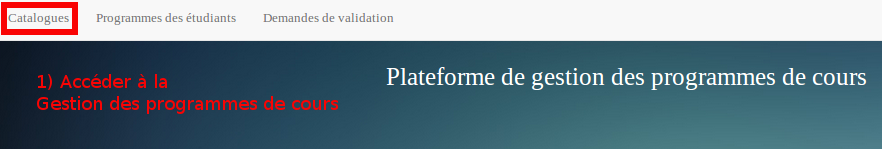
\includegraphics[width=\textwidth]{landing_page_access_to_catalog}
\caption{Accès de gestion des catalogues}
\label{fig:landing_page_catalog}
\end{figure}

Sur l'image ~\ref{fig:landing_page_catalog} apparaît la page d'accueil. Le menu pour accéder aux différents catalogues de cours est entouré d'un cadre rouge sur la capture d'écran. Les menus entourés du cadre bleu donnent accès aux différentes fonctionnalités offertes pour gérer les programmes des étudiants. Nous y reviendrons plus tard. 

\subsection{Accéder aux catalogues}
Après avoir cliquer sur le menu catalogue, nous arrivons sur la page montrant les différents cours présents dans l'application. Comme vous pouvez le voir sur la capture d'écran ~\ref{fig:catalog_index}, il n'y a qu'un seul catalogue pour le moment dans l'application. Vous pouvez cliquer sur la petite loupe en dessous de la colonne nommée \textit{info} pour accéder au catalogue en question ou sur la petite croix \textcolor{red}{rouge} pour le supprimer de l'application.

La section qui suit va expliquer les conventions à respecter lorsque l'on crée un graphe de cours avec yEd.

\begin{figure}
\centering
\caption{Liste des catalogues}
\label{fig:catalog_index}
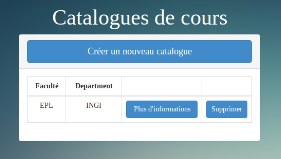
\includegraphics[width=\textwidth]{catalog_index}
\end{figure}

\subsection{Construction d'un catalogue de cours avec yEd}
Dans cette section nous allons pas à pas construire un graph de cours avec yEd (l'outil utilisé pour générer des graphes de cours).

Yed est disponnible ici \url{http://www.yworks.com/en/downloads.html\#yEd}

Nous allons créé un  catalogue de cours fictif, composé d'un programme, d'un module, de quelques cours et de quelques dépendances. Tout d'abord, ouvrez le programme yEd et créer un nouveau document. Une fois le yEd ouvert et le nouveau graph créer, vous verrez à votre droite le menu suivant ~\ref{fig:yed_menu}.

\begin{figure}[!htb]
\centering
\caption{Menu de yEd}
\label{fig:yed_menu}
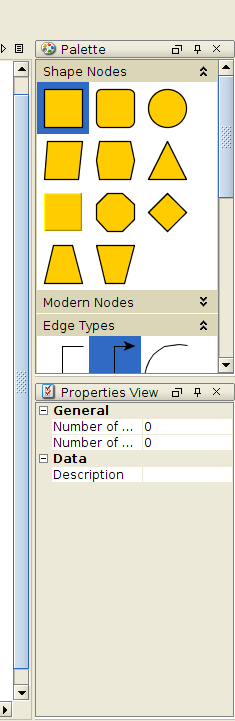
\includegraphics[scale=0.5]{yed_menu}
\end{figure}


\subsubsection{Créer des cours}
Pour créer les objets représentant les cours, il faut utiliser ce menu ~\ref{fig:yed_node_menu} et sélectionner le carré (en \textcolor{blue}{bleu sur la capture d'écran}) puis cliquer sur le document pour l'ajouter au graphe.

\begin{figure}
\centering
\caption{Menu de création des noeuds}
\label{fig:yed_node_menu}
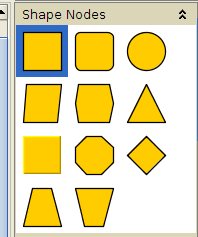
\includegraphics[scale=0.6]{yed_node_menu}
\end{figure}

Pour nommer le nœud:
\begin{enumerate}
\item Clique droit sur le nœud
\item Cliquez sur \textit{properties}
\end{enumerate}

Le menu suivant apparaîtra ~\ref{fig:properties_menu}. Il suffit de remplir le champ \textit{Texte} avec le nom désiré.

\begin{figure}
\centering
\caption{Ajouter un nom à un noeud}
\label{fig:properties_menu}
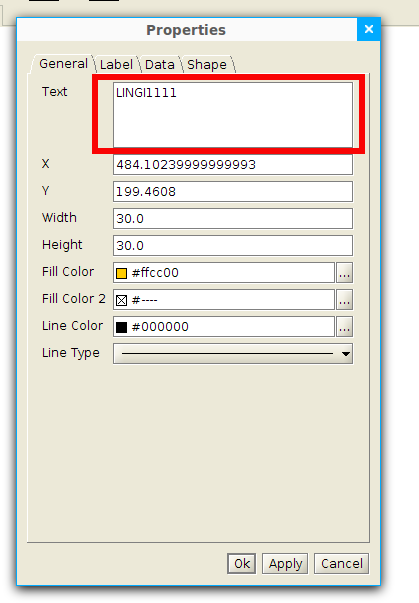
\includegraphics[scale=0.6]{properties_menu}
\end{figure}


\subsubsection{Ajouter des dépendances}

Pour représenter les dépendances entre les cours, il faut utiliser le menu présent sur l'image  ~\ref{fig:yed_edge_menu} qui permet de dessiner des arrêtes entre les nœuds.

\begin{figure}
\centering
\caption{Menu de création d’arêtes}
\label{fig:yed_edge_menu}
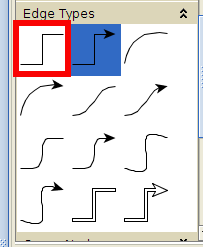
\includegraphics[scale=0.6]{yed_edge_menu}
\end{figure}

Nous utilisons deux type d’arêtes;

\begin{itemize}
\item en \textcolor{blue}{bleu} sur l'image ~\ref{fig:yed_edge_menu}, les arrêtes pour représenter les prérequis
\item en \textcolor{red}{rouge} sur l'image ~\ref{fig:yed_edge_menu}, les arrêtes pour représenter les corequis
\end{itemize}

Pour représenter les dépendances n-aire, l'application reconnait la convention suivante:

Simplement sélectionner un losange ou un rond, mettre le label \textbf{X pour représenter une contrainte disjonctive excusive (XOR)} ou {OR pour représenter une contrainte disjonctive (OR)} et la connecter aux différents cours concernés avec la contrainte (prérequis ou corequis) correspondante.

\begin{itemize}
\item Sur l'image \ref{fig:or_depandancy} est illustré à quoi doit ressembler une contrainte n-aire disjonctive.
\item Sur l'image \ref{fig:xor_depandancy} est illustré à quoi doit ressembler une contrainte n-aire disjonctive exclusive.
\end{itemize}

En créant un catalogue de deux cours, avec l'un étant le prérequis de l'autre, nous obtenons le graph présent sur l'image suivante ~\ref{fig:dependancies_example}.

\begin{figure}[!htb]
\centering
\caption{Prérequis n-aire disjonctif}
\label{fig:or_depandancy}
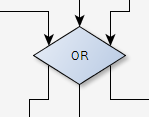
\includegraphics[scale = 1]{OR_dependancie}
\end{figure}

\begin{figure}[!htb]
\centering
\caption{Prérequis n-aire disjonctif exclusif}
\label{fig:xor_depandancy}
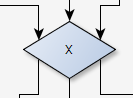
\includegraphics[scale = 1]{XOR_dependancie}
\end{figure}

\begin{figure}[!htb]
\label{fig:dependancies_example}
\centering
\caption{Deux cours avec une dépendance}
\includegraphics[scale=0.5]{dependancies_example}

\end{figure}

\subsubsection{Insérer des cours dans des modules}
Après avoir créer plusieurs cours, il est possible de regrouper ces nœuds dans une boite.
\begin{enumerate}
\item Sélectionner les noeuds à regrouper
\item Clique droit
\item Cliquer sur \textit{grouping}
\end{enumerate}

Vous obtiendrez une boite comme sur la capture ~\ref{fig:node_grouping}

\begin{figure}
\centering
\caption{Mettre des nœuds dans une boite}
\label{fig:node_grouping}
\includegraphics[scale=0.5]{node_grouping}
\end{figure}

La démarche à suivre pour nommer les boites est la même que celle pour nommer les nœuds.

Avant de poursuivre, il est nécessaire de préciser la structure de graph reconnue par l'application. 

\begin{itemize}
\item Un \textbf{catalogue} est représenté par un \textbf{graphe} et est composé exclusivement de \textbf{programmes}
\item Un \textbf{programme} est représenté par une \textbf{boite} et est composé de \textbf{modules} et de \textbf{cours}
\item Un \textbf{module} est représenté par une \textbf{boite} et est composé de plusieurs \textbf{sous-modules} et \textbf{cours}
\item Un \textbf{sous-module} marquera dans l'application tout les \textbf{cours} qu'il contient comme obligatoire pour le \textbf{module} parent.
\item Un \textbf{cours} est représenté par un \textbf{nœud} et peut avoir plusieurs dépendances. 
\item Une \textbf{dépendance} est représenté par une \textbf{arrête} entre deux \textbf{nœuds}.(Elle peut avoir deux type comme expliqué plus tôt
\end{itemize}

Sur l'image \ref{fig:small_catalog_example}, vous pouvez voir un exemple de catalogue valide.

\begin{figure}
\centering
\includegraphics[scale=0.6]{small_catalog_example}
\label{fig:small_catalog_example}
\caption{Un (petit) catalogue de cours valide}

\end{figure}

%*************************************************


\subsection{Création d'un catalogue - Import du graph dans l'application}
Une fois le graphe créé avec yEd, il ne reste plus qu'à créer un nouveau catalogue de cours en important ce graphe dans l'application. Depuis la page illustrée sur la capture d'écran \ref{fig:catalog_index}, cliquez sur \textbf{Créer un nouveau catalogue}.

Le formulaire qui permet de créer un nouveau catalogue est illustré sur la capture suivante \ref{fig:catalog_new}.

\begin{figure}
\centering
\caption{Création d'un catalogue de cours}
\label{fig:catalog_new}
\includegraphics[scale=0.6]{catalog_new}
\end{figure}

Remplissez, les champs (qui identifient votre catalogue), sélectionner le fichier de graph désiré et cliquez sur \textit{Créer le catalogue}

Vous arrivez sur la page présentée sur l'image suivante \ref{fig:catalog_show_manual}. Le bouton \textbf{Télécharger le fichier excel} permet de récupérer sous forme de formulaire excel les informations, à propos du catalogue de cours, qui sont contenues dans la base de données. Le bouton \textbf{Mettre à jour les informations} permet, quant à lui, de mettre à jour ces données avec le fichier Excel sélectionné avec me menu \textbf{choose file}.

\begin{figure}
\centering
\caption{Le catalogue une fois créé}
\label{fig:catalog_show_manual}
\includegraphics[width = \textwidth]{catalog_show_manual}
\end{figure}

\subsection{Mise à jour des informations contenues dans le catalogue}
Les informations contenue dans le graphe yEd n'étant pas complète, il est nécessaire, après avoir créer le catalogue, de compléter ses informations à l'aide d'un formulaire excel. Cette sous-section va expliquer les conventions à utiliser pour cela.

 


Pour ce faire il est conseillé  de \textbf{commencer par télécharger le formulaire Excel} (en cliquant sur le bouton en \textcolor{red}{rouge} sur l'image \ref{fig:catalog_show_manual}) contenant les informations du catalogue, les pages correctement nommées, ainsi que certaines proposition d'attributs à ajouter au catalogue. Il est préférable de ne pas passer cette étape. Dans le cas contraire, vous serez obligé d'écrire les identifiants de tout les différents programmes, modules et cours un à un dans le formulaire. Pour un catalogue de 55 cours, cela peut être long. 

Le formulaire est structuré comme suit:
\begin{itemize}
\item une page par objet cours, modules et programme;
\item la page relative au programme doit être nommée \textbf{PROGRAMMES};
\item la page relative au cours doit être nommée \textbf{COURS};
\item la page relative au modules doit être nommée \textbf{MODULES};
\item chaque colonne d'une page correspond à la propriété de l'objet en question;
\item le premier élément de chaque colonne (en \textbf{gras}) identifie le nom de la propriété (SIGLE pour la colonne relative aux sigles d'un cours par exemple);
\item les éléments sont identifiés en fonction de leur ligne dans le formulaire; le module d'import va chercher la colonne intitulé NAME (ou SIGLE si c'est un cours);
\item pour chaque élément de la colonne NAME (ou SIGLE), le module va rechercher l'objet qui est identifié par cette propriété, puis va ajouter un à un toute les propriétés se trouvant sur la même ligne que cet élément. 
\end{itemize}

Cette étape est répétable à l’infini. Ce pendant, faites attention à la cohérence des informations mises dans ce document. Le module d'import de fichiers Excel ne les détecte pas encore les incohérences qui peuvent y survenir. 

Remarques:
\begin{itemize}
\item il faut remplir coute que coute la colonne \textbf{SEMESTRE} de la page \textbf{COURSES} identifiant le semestre durant le quel est dispensé un cours (si cette propriété n'est pas définie, ils ne seront pas affichés aux étudiants);
\item attention à ne pas se tromper en utilisant les propriétés concernant les minimum et maximum de crédits d'un module ou d'un programme; un exemple d'incohérence serait un programme dont le maximum de crédits autorisés serait inférieur à la somme des minimum de crédits autorisés des modules qui le compose.
\end{itemize}



Une fois le \textit{template} de formulaire téléchargé et complété , sélectionnez le et cliquez sur le bouton \textit{Mettre à jour les informations} (en \textcolor{blue}{bleu} sur l'image \ref{fig:catalog_show_manual}).


Un message en \textcolor{blue}{bleu} vous avertira du succès de l'opération.


\subsection{Naviguer à travers les programmes de cours}

Pour inspecter les différents programmes ainsi que les modules et les cours qui le compose descendez sur la page \ref{fig:programs_index} et cliquez sur les différents onglets pour naviguer à travers les différents programmes, modules et cours. Tout cela se déroule sans devoir recharger la page. Pour obtenir encore plus d'information sur un cours, programme ou module, il suffit de cliquer sur la petite loupe en \textcolor{blue}{bleu}. Pour supprimer un élément, cliquez sur la croix \textcolor{red}{rouge}

\begin{figure}
\centering
\caption{Programmes, modules et cours}
\label{fig:programs_index}
\includegraphics[width = \textwidth]{programs_index}

\end{figure}



\section{Gestion des demandes de validations}
Lorsqu'un étudiant désire envoyer le programme qu'il s'est créé à la validation, une demande de validation est envoyé à la \textbf{commission INFO}. Pour accéder à ces demandes de validations, 
il suffit de cliquer sur le menu intitulé \textit{Validations} entouré en rouge sur l'image \ref{fig:landing_page_catalog}.

Sur la page des validations (Image~\ref{fig:validations}) vous pouvez:
\begin{itemize}
\item inspecter le programme que l'étudiant demande de valider en cliquant sur la petite loupe en \textcolor{blue}{bleu} (en dessous du menu \textbf{Programme});
\item accéder à la justification de l'étudiant en cliquant sur la petite loupe en \textcolor{blue}{bleu} (en dessous du menu \textbf{Justification});
\item valider la requête en cliquant sur \textit{Valider} (en \textcolor{green}{vert} sur l'image \ref{fig:validations});
\item refuser la requête en cliquant sur \textit{Refuser} (en \textcolor{red}{rouge} sur l'image \ref{fig:validations}).
\end{itemize}

\begin{figure}
\centering
\caption{Gestion des demandes de validations}
\label{fig:validations}
\includegraphics[scale=0.6]{validations}
\end{figure}
\subsection{Justification d'un étudiant}
Lorsque vous accéder au menu justification, vous arrivez sur la page illustrée sur la capture d'écran \ref{fig:justification_example}

\begin{figure}
\centering
\caption{Exemple de justification}
\label{fig:justification_example}
\includegraphics[width=\textwidth]{justification_example}
\end{figure}

Dans la colonne de gauche (\textbf{Description}) s'affiche toutes les contraintes non-respectée du programme de l'étudiant. 

Dans la colonne de droite (\textbf{Justification})s'affiche chacune des justifications de l'étudiant.

Tout en bas, un message peut être envoyé à l'étudiant, pour lui demander des informations supplémentaires par exemple. 

Le menu discussion de la page \ref{fig:landing_page_catalog} (dans les menus entourés d'un cadre \textcolor{blue}{bleu}) permet d'accéder directement à toute les justifications des étudiants.

\section{Gestion des années}

En cliquant sur le menu \textbf{Gérer les années} de la page \ref{fig:landing_page_catalog}, on accède à la page \ref{fig:manage_years} qui permet de gérer les années des étudiants. C'est ici que l'on peut marquer une année comme ratée ou réussie. 

Il est important de marquer les années après chaque année académique. Le statut des anciennes années est utilisé pour vérifier la validités des dépendances de cours. En effet, un prérequis dont le cours, présent dans une année ratée, n'a pas été crédité ne sera pas valide. 

\begin{figure}
\centering
\caption{Gérer les années des étudiants}
\label{fig:manage_years}
\includegraphics[width=\textwidth]{year_mgmt}
\end{figure}

Pour marquer une année comme réussie, il suffit de sélectionner l'action nommée \textbf{Réussie}. L'année et ses cours seront ainsi crédités. 

Lorsque l'on marque une année comme ratée, on arrive sur la page \ref{fig:fail_year}. Sur cette page, il faut sélectionner les cours qui ont été crédités.

\begin{figure}
\centering
\caption{Marquer une année comme ratée}
\label{fig:fail_year}
\includegraphics[width=\textwidth]{failed_year_mgmt}

\end{figure}



\end{document}